% Opcje klasy 'iithesis' opisane sa w komentarzach w pliku klasy. Za ich pomoca
% ustawia sie przede wszystkim jezyk oraz rodzaj (lic/inz/mgr) pracy.
\documentclass[english, mgr]{iithesis}

\usepackage[utf8]{inputenc}

%%%%% DANE DO STRONY TYTUŁOWEJ
% Niezaleznie od jezyka pracy wybranego w opcjach klasy, tytul i streszczenie
% pracy nalezy podac zarowno w jezyku polskim, jak i angielskim.
% Pamietaj o madrym (zgodnym z logicznym rozbiorem zdania oraz estetyka) recznym
% zlamaniu wierszy w temacie pracy, zwlaszcza tego w jezyku pracy. Uzyj do tego
% polecenia \fmlinebreak.
\englishtitle   {Domain-specific logic \fmlinebreak for terms with variable binding}
\polishtitle    {Logika dziedzinowa do wnioskowania \fmlinebreak o termach z~wiązaniem zmiennych}
\polishabstract {W~niniejszej pracy przyglądamy się fundamentalnej różnicy
między ręcznymi, a~komputerowymi systemami dowodowymi, zwracając uwagę na
wyzwanie, jakim jest utrzymanie precyzji i przejrzystości podczas
przeprowadzania matematycznego rozumowania w~obecności wiązania zmiennych.
W~praktyce, przy przenoszeniu dowodów przeprowadzonych na papierze do formalnych
i rygorystycznych komputerowych systemów dowodowych, potencjalne trudności
pojawiają się przy stosowaniu niejawnych założeń, a~w~szczególności przy
używaniu nieprecyzyjnego pojęcia ``wystarczająco świeżych'' nazw zmiennych.

Logika nominalna, wprowadzona przez Andrew M. Pittsa i oferująca pierwszorzędową
teorię nazw i wiązania zmiennych, jest jednym z~rozwiązań na wypełnienie tej luki.
Podejście to pozwala na zdefiniowanie podstawowych pojęć, w~tym
alfa-równoważności, świeżości i wiązania zmiennych,
wyłącznie w~kategoriach zamiany nazw,
odchodząc od klasycznych metod opartych na podstawieniu.

Bazując na pracy Pittsa, przedstawiamy wyspecjalizowaną odmianę logiki nominalnej,
w~której definiujemy więzy\-precyzyjne opisy własności syntaktycznych nazw i termów.
Kluczowym elementem naszej pracy jest algorytm ``Solver''\-narzędzie do automatycznego rozwiązywania więzów, będące jądrem sublogiki więzów i kompromisem pomiędzy
ludzkim i komputerowym stylem dowodzenia.
Do przeprowadzania rozumowań o więzach i innych własnościach syntaktycznych,
na fundamentach tej sublogiki zbudowaliśmy logikę wyższego rzędu,
w~której umieściliśmy więzy w~formułach i relacjach.

Dodatkowo zdefiniowaliśmy system i asystenta dowodzenia,
zainspirowane systemami dowodzenia z~rodziny HOL i zaimplementowane w~języku programowania OCaml.
Połączenie tych części składowych tworzy spójną strukturę służąca do precyzyjnego wyrażania
i rozumowania o złożonych właściwościach syntaktycznych,
której potencjał jako systemu do wnioskowania o językach programowania zademonstrowaliśmy
poprzez przeprowadzenie dowodu klasycznych własności rachunku lambda z~typami prostymi.
}
\englishabstract{In this work, we address a fundamental distinction between manual and computer-based proof systems, emphasizing the challenge of maintaining precision and transparency in handling variable binding. The common practice of making unspoken assumptions in pen-and-paper proofs, particularly the use of the imprecise notion of ``sufficiently fresh names,'' introduces potential pitfalls when translating to formal and rigorous proof systems.

Nominal Logic, as introduced by Andrew M. Pitts, emerges as a promising solution to bridge this gap, offering a first-order theory of names and binding. This approach allows for the definition of essential concepts, including alpha-equivalence, freshness, and variable binding, solely in terms of name swapping rather than classical renaming.

Building upon Pitts' work, we introduce a specialized variant of Nominal Logic, where we define constraints\-precise descriptors of syntactical properties—and use them to reason about terms with variable binding. We introduce ``The Solver''\-an algorithm for automated constraint resolution, which forms the logical core of the constraints sublogic and acts as a middle ground between human and computer provers. Layered on top of the constraints, we define a higher-order logic with constraints embedded into propositional formulas and relations.

Alongside this logic, we establish a proof system and a proof assistant implemented in OCaml and inspired by HOL theorem provers. The integration of these components forms a cohesive framework for the precise articulation of and reasoning about complex syntactic properties. To demonstrate its potential for reasoning within the programming languages world, we conduct proofs of classical properties of simply typed lambda calculus using this framework.
}
\author         {Dominik Gulczyński}
\advisor        {dr Piotr Polesiuk}
\date           {\today}                     % Data zlozenia pracy
% Dane do oswiadczenia o autorskim wykonaniu
\transcriptnum  {299391}                     % Numer indeksu
\advisorgen     {dr. Piotra Polesiuka} % Nazwisko promotora w dopelniaczu
%%%%%

%%%%% WLASNE DODATKOWE PAKIETY
\usepackage{amsmath}
\usepackage{amssymb}
\usepackage{stmaryrd} % For \llbracket
\usepackage{macros}
\usepackage{mathpartir}
\usepackage{mathtools}
\usepackage{listings}
\usepackage{semantic}
\usepackage{sourcecodepro}
\usepackage{enumitem}
\usepackage{tabularx}
\usepackage{makecell}
\usepackage{mdframed}
\usepackage{hyperref}
\usepackage{subcaption}
\usepackage[toc,page]{appendix}
\usepackage{multicol}
\usepackage{multirow}
\usepackage{graphicx}
\usepackage{pgf}
\usepackage{tikz-qtree}

%%%%% WŁASNE DEFINICJE I POLECENIA
\definecolor{codegreen}{rgb}{0,0.6,0}
\definecolor{codegray}{rgb}{0.5,0.5,0.5}
\definecolor{codepurple}{rgb}{0.58,0,0.82}
\definecolor{backcolour}{rgb}{0.95,0.95,0.92}
\lstdefinestyle{ocamlstyle}{
    commentstyle=\color{codegreen},
    escapebegin=\color{black},
    keywordstyle=\color{magenta},
    numberstyle=\tiny\color{codegray},
    stringstyle=\color{codepurple},
    basicstyle=\ttfamily\footnotesize,
    breakatwhitespace=false,
    breaklines=true,
    captionpos=b,
    keepspaces=true,
    numbersep=5pt,
    showspaces=false,
    showstringspaces=false,
    showtabs=false,
    tabsize=2
}
\lstset{style=ocamlstyle}
\lstdefinelanguage{OCaml}[]{caml}{
    morekeywords={val, ProofEnv, otherwise, private},
    otherkeywords = {|>, \%>, +=, -=, ->, ::}
}
\setlist{nolistsep}
\renewcommand{\sc}[1]{\textsc{\small{#1}}}
\renewcommand{\tt}[1]{\texttt{\small{#1}}}
\newcommand{\lstt}[1]{\text{{\lstinline[columns=fixed,mathescape]|#1|}}}
\renewcommand{\it}[1]{\textit{#1}}
\newcommand{\aequiv}{\ensuremath{=_\alpha}}
\newcommand{\solverRule}{\vdash}
\newcommand{\NeqAtoms}{\tt{neq\_atoms}}
\newcommand{\Fresh}{\tt{fresh}}
\newcommand{\VarShape}{\tt{var\_shape}}
\newcommand{\Shape}{\tt{shape}}
\newcommand{\Subshape}{\tt{subshape}}
\newcommand{\Symbols}{\tt{symbols}}
\newcommand{\TransferShape}{\tt{transfer\_shape}}
\newcommand{\Assumptions}{\tt{assumptions}}
\newcommand{\occurs}[2]{\ensuremath{ {#1}\text{ occurs in }{#2}}}
\newcommand{\stxoccurs}[2]{\ensuremath{ {#1}\text{ occurs syntactically in }{#2}}}
\newcommand{\pluseq}{\mathrel{+}=}
\newcommand{\minuseq}{\mathrel{-}=}
\newcommand{\shrep}[2][\icEnv]{\ensuremath{ #2_{#1}}}
\newcommand{\shenv}[2][\icEnv]{\ensuremath{ |#2|_{#1}}}
\newcommand{\fix}[3]{\ensuremath{\text{fix }#1(#2)\ofkind#3=}}\newcommand{\myatop}[2]{\ensuremath{\genfrac{}{}{0pt}{}{#1\hfill}{#2\hfill}}}
\newcommand{\scbrk}[2]{\myatop{\textsc{#1}}{\textsc{#2}}}
\newcommand{\hole}{\ensuremath{\bullet}}
\newcommand{\mdash}{\,---\,}
\def\-{{\mdash}}

\newcolumntype{L}{X}
\newcolumntype{C}{>{\centering\arraybackslash}X}
\newcolumntype{R}{>{\raggedleft\arraybackslash}X}

\usepackage[backend=bibtex,sorting=ynt]{biblatex}
\addbibresource{references.bib}
\selectlanguage{english}

%%%%%%%%%%%%%%%%%%%%%%%%%%%%%%%%%%%%%%%%%%%%%%%%%%%%%%%%%%%%%%%%%%%%%%%%%%%%%%%%

\begin{document}

%%%%%%%%%%%%%%%%%%%%%%%%%%%%%%%%%%%%%%%%%%%%%%%%%%%%%%%%%%%%%%%%%%%%%%%%%%%%%%%%
\chapter{Introduction}
% \section{Motivation}
One of the fundamental distinctions between conducting proofs manually with pen and paper
and using a computer lies in the flexibility and liberties one can take in the first case.
Human provers and reviewers often agree upon unexplained or unproven assumptions
and may skip some unimportant boilerplate.
Computers, on the other hand, are less forgiving
and demand transparency and justification down to the smallest details.

An assumption we commonly make when writing pen-and-paper proofs pertains to
working with abstract syntax trees,
where we assume that the variables we choose are fresh enough
or that substitutions avoid issues like variable capture.
For instance, when dealing with lambda calculus, we often construct inductive proofs
over the structure of an expression. In the case of an abstraction, we will implicitly only show
the scenario where the variable bound in that abstraction is \it{sufficiently fresh}.
Addressing the general case could introduce unnecessary complexities unrelated to the theorem at hand.
Justifiably, we skip over this detail\-however, the induction principle obliges us to prove the case for arbitrary variable names.

Addressing this gap in formal reasoning requires careful considerations to come up with a resolution.
Fortunately, there exist some solutions to that problem\-and one particular
approach, coined \it{nominal logic} and introduced by Andrew M. Pitts\cite{nominal-logic}, is of most interest to this work.


\section{Nominal approach}
Pitts' work introduces \it{nominal logic}, a first-order theory of names, swapping, and freshness,
that, among other novelties, provides a precise mathematical definition
describing the concept of "sufficiently fresh names",
which, as Pitts argues, bridges the gap between formal mathematical reasoning and the informal practices mentioned earlier.

Pitts chose to found his theory around the notion of swapping names
as opposed to the classical renaming.
In the author's previous work\cite{abstract-syntax-variable-binding}, written together with Murdoch J. Gabbay,
it was shown that a theory based on this operation allows for all necessary concepts,
including alpha-equivalence, freshness, and variable-binding,
to be defined solely in terms of swapping pairs of names.

\begin{mdframed}[frametitle={\textnormal{\footnotesize \textbf{\citeauthor{nominal-logic}}, \textit{\citetitle{nominal-logic}}\cite{nominal-logic}:}}]
Names of what? Names of entities that may be subject to binding by some of
the syntactical constructions under consideration. In Nominal Logic these sorts of
names, the ones that may be bound and hence that may be subjected to swapping
without changing the validity of predicates involving them, will be called atoms.
\end{mdframed}

Additionally, swapping has one other useful logical property\-it is involutive
(i.e. a swap gets nullified by applying the same swap again, while substitutions cannot always be reversed),
which, as Pitts argues, means that \it{equivariant} predicates
(i.e. those whose validity is invariant under name-swapping)
have excellent logical properties.
This class of equivariant predicates includes equality, alpha-equivalence and is
closed under standard logical connectives, universal and existential quantification,
and formation of least and greatest fixpoint.

\begin{figure}[htbp]
  \centering
  \begin{tabularx}{\textwidth}{|CXr|}
      \hline & & \\
  $ t \; \deff \; a \mid \lambda a . t \mid t\;t $
  & & (lambda terms)
  \\ & & \\ \hline
\end{tabularx}
  \caption{Terms of untyped lambda calculus.}
  \label{fig:lambda-calculus}
\end{figure}
As an example of Nominal Logic at work, consider the abstract syntax tree of untyped lambda calculus,
given by the grammar above, where $a$ ranges over an infinite set of names\-or rather \it{atoms}.

\begin{figure}[htbp]
  \centering
  \begin{tabularx}{\textwidth}{|RC|}
      \hline & \\
      \begin{tabular}{rcl}
      $\permswap{a}{b}{(\lambda c . t)} $ & $:=$
      & $ \lambda (\permswap{a}{b}{c}) . (\permswap{a}{b}{t})$ \\
      $\permswap{a}{b}{(t_1\; t_2)} $ & $:=$
      & $ (\permswap{a}{b}{t_1}) \; (\permswap{a}{b}{t_2}) $
      \end{tabular}
      &
      $\permswap{a}{b}{c} \;\: := \;\: \begin{cases}
          a & \text{if } c = b \\
          b & \text{if } c = a \\
          c & \text{otherwise}
        \end{cases}$
      \\ &  \\
      \hline
\end{tabularx}
  \caption{Swapping procedure.}
  \label{fig:swap}
\end{figure}
The definition of swapping atoms $a$ and $b$ in some tree $t$,
written $\permswap{a}{b}{\:t}$, is rather straightforward\-it naturally follows the tree structure, touching only the affected atoms,
and doesn't need to distinguish between free and bound names (like substitutions do),
but simply changes them all the same exact way.

\pagebreak

\begin{figure}[htbp]
  \centering
    \begin{tabularx}{\textwidth}{|CCCC|}
      \hline & & & \\
      $
      \inference{
        a \cneq b
      }{
        a \cfresh b
      }
      $ & $
      \inference{
        a \cfresh t_1 & a \cfresh t_2
      }{
        a \cfresh t_1\;t_2
      }
      $ & $
      \inference{
      }{
        a \cfresh \lambda a . t
      }
      $ & $
      \inference{
        a \cfresh t
      }{
        a \cfresh \lambda b . t
      }
      $ \\ & & & \\ \hline
    \end{tabularx}
  \caption{Freshness relation.}
  \label{fig:fresh}
\end{figure}
Relation of \it{freshness} of atom $a$ in tree $t$, written $a \cfresh t$,
is similarly simple to define.\footnote{Pitts defines it as
$a$ not being a member of the \it{support set} of $t$. For our purposes, the simple inductive definition will suffice.}\
Note that it only assumes the comparability of atoms
and is an \it{equivariant} relation, which can be shown by simplest induction.

\begin{figure}[htbp]
  \centering
    \begin{tabularx}{\textwidth}{|ccCcc|}
    \hline & & & & \\ {} &
    $
    \inference{
      \text{}
    }{
      a \aequiv a
    }
    $ & $
    \inference{
      t_1 \aequiv t_1' & t_2 \aequiv t_2'
    }{
      t_1\;t_2 \aequiv t_1'\;t_2'
    }
    $ & $
    \inference{
      \permswap{a}{b}{t} \aequiv \permswap{a'}{b}{t'} & b \cfresh t & b \cfresh t'
    }{
      \lambda a . t \aequiv \lambda a' . t'
    }
    $ & {} \\ & & & & \\ \hline
    \end{tabularx}
  \caption{Alpha-equivalence relation.}
  \label{fig:fresh}
\end{figure}
With \it{swapping} and \it{freshness} already established,
we define the alpha-equivalence of terms, written $t_1 \aequiv t_2$.
We built this definition of alpha-equivalence using only induction,
swapping, and freshness then, as Pitts argues, it is equivariant as well.
\\
\begin{mdframed}[frametitle={\textnormal{\footnotesize \textbf{\citeauthor{nominal-logic}}, \textit{\citetitle{nominal-logic}}\cite{nominal-logic}:}}]
The fundamental assumption underlying Nominal Logic is that \textit{the only predicates we ever deal with} (when describing properties of syntax) \textit{are equivariant ones, in the sense that their validity is invariant under swapping} (i.e., transposing, or interchanging) \textit{names}.
\end{mdframed}

\section{Motivation and contributions}
Nominal logic opens avenues for expressing alpha-equivalence, freshness, and
other fundamental syntactic properties with elegance.
Formalizing theories within such a system calls for
a robust framework, ideally accompanied by a proof assistant.
To achieve the bigger goal of abstracting away the mundane handling of these
properties, which are so obvious to the human eye,
yet non-trivial from the point of view of rigorous computer accuracy,
we strive for an automatic deductive process.

We categorize the fundamental properties of terms with variable binding,
such as alpha-equivalence and freshness, as \it{constraints}.
As a middle ground between human and computer provers,
we introduce \it{the Solver}, an algorithm designed to automatically
resolve new constraints based on the pre-established ones.
It serves as the logical core of the constraints sub-logic,
that together with the embedding of constraints into propositional formulas
constructs a higher-order logic capable of seamlessly expressing these properties.
This approach liberates users from the painstaking task of manually proving the seemingly trivial but crucial details,
through automated resolution of constraints,
while ensuring the completeness and correctness of written proofs.

For the user interface, we have developed a proof checker and proof assistant,
tying all the parts together in a cohesive framework.
The proof assistant draws inspiration from the HOL family of theorem provers,
initially introduced by Michael J. C. Gordon\cite{HOL}.
Similar to HOL, it utilizes the OCaml programming language as the
interface to writing proofs and encoding theorems.
While currently somewhat low-level, with further automation efforts,
it should achieve intuitiveness and user-friendliness akin to other,
more mature and powerful proof assistants.

\section{Related work}
Of course, there are other works that focus on reasoning about
syntactical properties of binders, as they are essential
in formalizing properties of programming languages.

\begin{itemize}
\item \textbf{Higher-Order Abstract Syntax} (HOAS), introduced by Frank Pfenning
and Conal Elliott\cite{hoas}, is a uniform and generic representation of terms, formulas, programs, and other
syntactic objects used in formal reasoning systems that focus on substitution and
unification under the presence of binders. The authors utilize the binding construct of the implementation language to represent the binding in the language being formalized.
\\

\item  \textbf{Twelf}\cite{twelf} is a framework used to specify, implement, and prove properties of deductive systems and logics, that encodes HOAS within the \textbf{LF} logical framework\cite{LF},
by utilizing its own constraint logic programming language Elf.
The principal authors of Twelf are Frank Pfenning and Carsten Schürmann.
Multiple research projects were developed using it, including a type safety proof for Standard ML\cite{twelf-ml}.
\\

\item  \textbf{Beluga}\cite{beluga} is a programming framework designed for reasoning about formal systems,
that is also based on the LF logical framework.
It encodes the HOAS approach using dependent types and provides support for reasoning with context and contextual objects.
It's developed at the Complogic group at McGill University, led by Brigitte Pientka.
One of the case studies of using Beluga was mechanization of logical relations by
contextual types\cite{beluga-relations}.
\\

\item \textbf{Parametric Higher-Order Abstract Syntax} (PHOAS) improves
on the idea of HOAS by utilizing dependently-typed abstract syntax trees to
formalize it in general-purpose type theories, like Coq's Calculus of Inductive Constructions.
Introduced by Adam Chlipala\cite{phoas}, it has been used to develop certified, executable program transformations over several formalizations of statically-typed functional programming languages.
\\

\item \textbf{Locally Nameless Representation} is
an approach to the representation of syntax with variable binders,
introduced by Arthur Charguéraud\cite{locally-nameless}.
It represents the bound variables through de Bruijn indices, while retaining
names of the free variables, achieving strong induction principles.
Utilizing the Coq library TLC developed by Charguéraud, the approach has successfully formalized diverse type systems and semantics.
\\

\item \textbf{Autosubst}\cite{autosubst}
is a Coq library that automates some crucial parts of formalizing syntactic theories with variable binders,
developed by Steven Schäfer, Tobias Tebbi, and Gert Smolka.
Authors employ de Bruijn representation of terms with additional binding annotations
to automatically derive the substitution operation and proofs of substitution lemmas.
They introduce an automation tactic that solves equations involving terms and substitutions,
based on their work on the decision procedure of the equational theory of
an extension of the sigma-calculus by Abadi et al\cite{sigma-calculus}.
\\

\end{itemize}
%%%%%%%%%%%%%%%%%%%%%%%%%%%%%%%%%%%%%%%%%%%%%%%%%%%%%%%%%%%%%%%%%%%%%%%%%%%%%%%%
\chapter{Terms and constraints}
To properly describe our framework and constraints sublogic,
we must start with the simplest elements: \it{names}, \it{terms}, and \it{constraints}.

\begin{figure}[htbp]
  \centering
  \framebox[\textwidth]{
    \begin{tabularx}{\textwidth}{rcl@{\extracolsep{\fill}}r}
      $\perm$    & $\deff$ & $\permid
                          \mid \permswap{\atomexp}{\atomexp}{\perm}$
      & (permutations) \\
      $\atomexp$ & $\deff$ & $\perm \apperm \atomv$
      & (atom expressions) \\
      $\term$    & $\deff$ & $\atomexp
                         \mid \perm \apperm \termv
                         \mid \tbind{\atomexp} \term
                         \mid \term \tapp \term
                         \mid \symb$
      & (terms) \\
      $\constr$  & $\deff$ & $\atomexp \cfresh \term
                         \mid \term \ceq \term
                         \mid \term \csheq \term
                         \mid \term \cshlt \term
                         \mid \csymb \term$
      & (constraints) \\
      $\shape$ & $\deff$ & $\shatom
                     \bnfor \termv
                     \bnfor \shbind \shape
                     \bnfor \shape \tapp \shape
                     \bnfor \symb$
      & (shapes) \\
    \end{tabularx}
  }
  \caption{Syntax of constraint sublogic.}
  \label{fig:terms-constraints-syntax}
\end{figure}
The names are drawn from an infinite set of \it{atoms} (represented by lowercase letters)
and correspond to the bound variables in terms, analogous to the variables in lambda calculus.
This set is disjoint from the set of variables commonly used in first-order logic,
which we will refer to as \it{variables} (denoted by uppercase letters).

The terms are constructed to mimic the structure of abstract syntax trees of the lambda calculus,
extending it with the notion of permutations (of atoms) and functional symbols,
denoted by the metavariable $\symb$, drawn from yet another set disjoint from atoms and variables.
The construction $\tbind{\atomexp} \term$ represents a \it{binder}\-informally, we think of it as binding the occurrences of $\atomexp$ in $\term$,
similarly to a lambda abstraction\-yet it \it{isn't} a binder,
but a simple syntactical construction gluing together an atom with a term.
The semantics of binding will apply only in the interpretation of this syntactical term in the model.
Note that we do not restrict this construction to the form of $\tbind{\atomv} \term$, but allow permuted atoms to appear on the left side of the binders.

\begin{figure}[htbp]
  \centering
  \begin{tabularx}{\textwidth}{|C|}
    \hline
    \begin{subfigure}{0.45\textwidth}
      \begin{eqnarray*}
        \perm \apperm (\perm' \apperm \atomv)  & := & (\perm \++ \perm') \apperm \atomv \\
        \perm \apperm (\perm' \apperm \termv)  & := & (\perm \++ \perm') \apperm \termv \\
        \perm \apperm (\tbind{\atomexp} \term) & := & \tbind{(\perm \apperm \atomexp)} (\perm \apperm \term) \\
        \perm \apperm (\term_1 \tapp \term_2)  & := & (\perm \apperm \term_1) \tapp (\perm \apperm \term_2) \\
        \perm \apperm \symb                    & := & \symb \\
      \end{eqnarray*}
    \end{subfigure}
    \begin{subfigure}{0.45\textwidth}
      \begin{eqnarray*}
        \shapeof{\perm \apperm \atomv}   & := & \shatom \\
        \shapeof{\perm \apperm \termv}   & := & \termv  \\
        \shapeof{\tbind{\atomexp} \term} & := & \shbind \shapeof{\term} \\
        \shapeof{\term_1 \tapp \term_2}  & := & \shapeof{\term_1} \tapp \shapeof{\term_2} \\
        \shapeof{\symb}                  & := & \symb \\
      \end{eqnarray*}
    \end{subfigure}
  \\ \hline
  \end{tabularx}
  \caption{Description of applying a permutation and taking shape.}
  \label{fig:permutation-shapes-interpretation}
\end{figure}
Additionally, when dealing with atom expressions with the identity permutation $\permid \;\atomv$,
we will skip the permutation and simply write $\atomv$,
and sometimes call such atom expressions \it{pure}.
Although permutations only affect atoms, they are also stored within variables.
When the variable is substituted for a term, we apply that permutation
on the substituted term.
We also define the term shapes and how to compute them, which
we will use to resolve constraints.
We do not define the operation of ``applying'' a swap permutation on
an atom, as it is never explicitly utilized within our framework;
permuted atoms are handled through the Solver rules instead.
However, the notion of applying swaps is included in the
model definition.

The constraints are precise descriptions of syntactical properties,
describing the relationship between their arguments\-atoms and terms.
It's crucial to emphasize that these terms and constraints function
solely as data structures and do not incorporate notions of binding or reduction by themselves.
These properties can only appear after we interpret
constraints within the logical model, which allows us to then reason about
concepts such as \it{freshness}, \it{variable binding}, and \it{structural} order.
\begin{figure}[hbtp]
  \centering
  \begin{tabularx}{\linewidth}{|l|X|}
    \hline
    $\atomexp \cfresh \term$ & Atom $\atomexp$ is fresh in term $\term$, meaning it does not occur in $\term$ as a free variable. \\
    \hline
    $\term_1 \ceq \term_2$ & Terms $\term_1$ and $\term_2$ are alpha-equivalent. \\
    \hline
    $\term_1 \csheq \term_2$ & Terms $\term_1$ and $\term_2$ possess an identical shape, i.e., after erasing all atoms, terms $\term_1$ and $\term_2$ would be equal. \\
    \hline
    $\term_1 \cshlt \term_2$ & The shape of term $\term_1$ is structurally smaller than the shape of term $\term_2$, i.e., after erasing all atoms, $\term_1$ would be equal to some subterm of $\term_2$. \\
    \hline
    $\csymb \term$ & term $\term$ is equal to some functional symbol. \\
    \hline
  \end{tabularx}
  \caption{Informal semantics of constraints.}
  \label{fig:informal-constraints-semantics}
\end{figure}

\section{Model}
\begin{figure}[htbp]
  \centering
  \framebox[\textwidth]{
    \begin{tabularx}{\textwidth}{rcl@{\extracolsep{\fill}}r}
      $\semterm$ & $\deff$ & $\sematom
                        \bnfor n
                        \bnfor \stbind \semterm
                        \bnfor \semterm \stapp \semterm
                        \bnfor \symb$
      & (semantic terms) \\
      $\semshape$ & $\deff$ & $\shatom
                        \bnfor \stbind \semshape
                        \bnfor \semshape \stapp \semshape
                        \bnfor \symb$
      & (semantic shapes)
    \end{tabularx}
  }
  \caption{Semantic representation of terms and shapes.}
  \label{fig:semantic-terms-shapes}
\end{figure}
To build the mathematical model of terms and constraints,
we introduce \it{semantic terms} and \it{semantic shapes} that will inhabit it.
We will use metavariable $\sematom$ for \it{semantic names} drawn from an
infinite set of names, representing the free variables.
Binders in semantic terms are achieved by De Bruijn indices\cite{deBruijn}, and consequently,
the bound names are represented by natural numbers, denoted by $n$,
and the binding construction has no explicit argument, denoted by $\stbind$.

\begin{figure}[htbp]
  \centering
  \begin{tabularx}{\textwidth}{|C|}
    \hline
    \begin{subfigure}{0.45\textwidth}
      \begin{eqnarray*}
        \termMdl{\perm \apperm \atomv}{\tmEnv} & := &
          \permMdl{\perm}{\tmEnv}(\tmEnv(\atomv)) \\
        \termMdl{\perm \apperm \termv}{\tmEnv} & := &
          \permMdl{\perm}{\tmEnv}(\tmEnv(\termv)) \\
        \termMdl{\tbind{\atomexp} \term}{\tmEnv} & := &
          \stbind (\termMdl{\term}{\tmEnv} \shiftIdx)
            \subst{\termMdl{\atomexp}{\tmEnv}}{0} \\
        \termMdl{\term_1 \tapp \term_2}{\tmEnv} & := &
          \termMdl{\term_1}{\tmEnv} \stapp \termMdl{\term_2}{\tmEnv} \\
        \termMdl{\symb}{\tmEnv} & := & \symb \\
      \end{eqnarray*}
    \end{subfigure}
    \begin{subfigure}{0.45\textwidth}
      \begin{eqnarray*}
        \shapeof{\sematom}                     & := & \shatom \\
        \shapeof{n}                            & := & \shatom \\
        \shapeof{\stbind \semterm}             & := & \stbind \shapeof{\semterm} \\
        \shapeof{\semterm_1 \stapp \semterm_2} & := &
          \shapeof{\semterm_1} \shapp \shapeof{\semterm_2} \\
        \shapeof{\symb}                        & := & \symb \\
      \end{eqnarray*}
    \end{subfigure}
    \\ \vspace{-8mm}
    \begin{subfigure}{0.47\textwidth}
      \begin{eqnarray*}
        \permMdl{\permid}{\tmEnv}(\sematom) & := & \sematom \\
        \permMdl{\perm \++ \swap{\atomexp_1}{\atomexp_2}}{\tmEnv}(\sematom)   & := & \permMdl{\perm}{\tmEnv} (\sematom') \\
        \text{where }\; \sematom' & := &  \permMdl{\permswap{\atomexp_1}{\atomexp_2}{}}{\tmEnv}(\sematom)  \\
        & & \\
      \end{eqnarray*}
    \end{subfigure}
    \begin{subfigure}{0.43\textwidth}
      \begin{eqnarray*}
        \permMdl{\permswap{\atomexp_1}{\atomexp_2}{}}{\tmEnv}(\sematom)  & := &
          \begin{cases}
            \sematom_2 & \text{if } \sematom = \sematom_1 \\
            \sematom_1 & \text{if } \sematom = \sematom_2 \\
            \sematom   & \text{otherwise}
          \end{cases} \\
        \text{where }\: \sematom_1 & := &  \permMdl{\atomexp_1}{\tmEnv} \\
        \text{  and }\: \sematom_2 & := &  \permMdl{\atomexp_2}{\tmEnv} \\
      \end{eqnarray*}
    \end{subfigure}
    \\ \hline
  \end{tabularx}
  \caption{Interpretation of terms and shapes in the model.}
  \label{fig:terms-shapes-interpretation}
\end{figure}
The term interpretation function, denoted $\termMdl{\cdot}{\tmEnv}$,
maps syntactic terms to semantic terms,
utilizing the standard shifting of De Bruijn indices (denoted by $\cdot\shiftIdx$).
It is parametrized by the function $\tmEnv$ that maps atoms and variables to
semantic atoms and terms.
The shape interpretation function, denoted $\shapeof{\cdot}$,
maps semantic terms to semantic shapes by erasing names.

\begin{figure}[htbp]
  \centering
    \begin{tabularx}{\textwidth}{|XlclX|}
      \hline & & & & \\
      & $\tmEnv \vDash \term_1 \ceq \term_2 $  & \textrm{iff} &
        $\termMdl{\term_1}{\tmEnv} = \termMdl{\term_2}{\tmEnv}$ & \\
      & $\tmEnv \vDash \atomexp \cfresh \term$ & \textrm{iff} &
        $\termMdl{\atomexp}{\tmEnv} \notin
          \mathsf{FreeAtoms}(\termMdl{\term}{\tmEnv})$ & \\
      & $\tmEnv \vDash \term_1 \csheq \term_2$ & \textrm{iff} &
        $\shapeof{\termMdl{\term_1}{\tmEnv}} = \shapeof{\termMdl{\term_2}{\tmEnv}}$ & \\
      & $\tmEnv \vDash \term_1 \cshlt \term_2$ & \textrm{iff} &
        $\shapeof{\termMdl{\term_1}{\tmEnv}} \textrm{ is a strict subshape of }
          \shapeof{\termMdl{\term_2}{\tmEnv}}$ & \\
      & $\tmEnv \vDash \csymb \term$ & \textrm{iff} &
        $\shapeof{\termMdl{\term}{\tmEnv}} \textrm{ is a functional symbol }$ & \\
      & & & & \\ \hline
    \end{tabularx}
  \caption{Interpretation of constraints in the model.}
  \label{fig:constraint-interpretation}
\end{figure}
With the above machinery, we establish the relation $\tmEnv \vDash \constr$
that interprets the constraints in our model, using some mapping $\tmEnv$.
As a consequence of using De Bruijn indices, we can trivially compute the
$\mathsf{FreeAtoms}(\semterm)$ set and use it to check freshness.
Note that it's possible for terms of the form $\tbind{a}{X}$ and $\tbind{b}{Y}$
to be equal in this model.

\pagebreak

We will use metavariable $\cEnv$ to represent finite sets of constraints,
and write $\tmEnv \vDash \cEnv$ if for all $\constr \in \cEnv$,
we have $\tmEnv \vDash \constr$,
as well as write $\cEnv \vDash \constr$ if for every $\tmEnv$ such that $\tmEnv \vDash \cEnv$,
we have $\tmEnv \vDash \constr$.
In the next chapter, we present the deterministic \it{Solver} algorithm
that emulates this model by syntactically verifying statements of the form $\cEnv \vDash \constr$.

%%%%%%%%%%%%%%%%%%%%%%%%%%%%%%%%%%%%%%%%%%%%%%%%%%%%%%%%%%%%%%%%%%%%%%%%%%%%%%%%
\chapter{Constraint solver} \label{sec:solver}
At the heart of our work lies the Solver, an algorithm designed to resolve constraints.
For any assumed constraints $\constr_1, \dots, \constr_n$, and
goal constraint $\constr_0$, the Solver determines whether the judgment $\constr_1, \dots, \constr_n \vDash \constr_0$ holds.
Meaning that for every possible substitution of variables into closed terms in constraints $\constr_0, \constr_1, \dots, \constr_n$,
such that $\constr_1, \dots, \constr_n$ are satisfied, would also satisfy $\constr_0$.

\begin{figure}[htbp]
  \centering
  \framebox[\textwidth]{
    \begin{tabularx}{\textwidth}{rcl@{\extracolsep{\fill}}r}
      $\sconstr$ & $\deff$ & $\atomexp \cfresh \term
                       \bnfor \term \ceq \term
                       \bnfor \shape \csheq \shape
                       \bnfor \shape \cshlt \shape
                       \bnfor \csymb \term$
      & (solver constraints)
    \end{tabularx}
  }
  \caption{Solver's internal representation of constraints.}
  \label{fig:solver-internal-representation}
\end{figure}
For the sake of convenience and implementation efficiency, the Solver operates
on its own internal representation of constraints, which slightly differs from
constraints described in the previous section.
It erases atoms in terms under shape constraints,
effectively transforming them into \it{shapes}.
Moreover, we define some syntactic sugar.
\begin{figure}[htbp]
    \centering
    \begin{tabularx}{\textwidth}{|CC|}
      \hline & \\
      \begin{tabular}{rcl}
        $\atomv \cneq \atomexp $ & $:=$ & $\atomv \cfresh \atomexp$ \\
        $(\perm \apperm \atomv) \cfresh \term $ & $:=$ & $\atomv \cfresh \perm^{-1} \apperm \term $ \\
      \end{tabular}
      &
      \begin{tabular}{rcl}
      $ \permid ^ {-1} $& $:=$ & $\permid $ \\
      $ (\permswap{\atomexp_1}{\atomexp_2} \perm) ^ {-1} $ & $:=$ & $\perm^{-1} \++ \permswap{\atomexp_1}{\atomexp_2}
      $\\
      \end{tabular}
      \\ & \\ \hline
      \end{tabularx}
  \caption{Desugaring of constraints' syntax.}
  \label{fig:symbol-rules}
\end{figure}

A high-level perspective of the Solver is that it works on judgments of the form
$\cEnv; \icEnv \solverRule \sconstr$, verifying whether a given goal-constraint $\sconstr$
holds in environments of assumed constraints (kept in $\cEnv$ and $\icEnv$)
by dissecting constraints on both sides of the turnstile into
irreducible components that are straightforward to handle.
\begin{figure}
  \centering
  \begin{tabularx}{\textwidth}{|l|X|}
    \hline
    $\atomv_1 \cneq \atomv_2$
    & Atoms $\atomv_1$ and $\atomv_2$ are different.
    \\ \hline
    $\atomv   \cfresh \termv$
    & Atom $\atomv$ is {Fresh} in variable $\termv$.
    \\ \hline
    $\termv_1 \csheq  \termv_2$
    & Variables $\termv_1$ and $\termv_2$ posses the same shape.
    \\ \hline
    $\termv   \csheq  \term$
    & Variable $\termv$ has a shape of term $\term$.
    \\ \hline
    $\term    \cshlt  \termv$
    & Term $\term$ strictly subshapes variable $\termv$.
    \\ \hline
    $\csymb \termv$
    & Variable $\termv$ is some functional symbol.
    \\ \hline
  \end{tabularx}
  \caption{Irreducible constraints.}
  \label{fig:irreducible-constraints}
\end{figure}

Environment $\cEnv$ keeps the yet unprocessed assumptions,
while another environment $\icEnv$ keeps track of already analyzed and irreducible assumptions.
These assumptions usually flow from the former to the latter, but if we analyze
a constraint that affects other assumptions in $\icEnv$,
they may flow back to $\cEnv$ to be further dissected by the Solver.
After all assumptions in $\cEnv$ are reduced to irreducible constraints,
we break down the goal-constraint $\sconstr$ and repeat the reduction procedure on
new assumptions and the goal.
\begin{figure}[htpb]
  \centering
    \begin{tabularx}{\textwidth}{|CCCC|}
    \hline & & \\ $
      \inference{
      }{
        \cEnv ; \lightning \solverRule \sconstr
      }
      $ & $
        \cEnv \vDash \sconstr \;\equiv\;
        \cEnv ; \emptyenv \solverRule \sconstr
      $ & $
      \inference{
        \sconstr \text{ is trivial}
      }{
        \emptyenv ; \icEnv \solverRule \sconstr
      } $ & $
      \inference{
        \sconstr \in \icEnv
      }{
        \emptyenv ; \icEnv \solverRule \sconstr
      } $ \\ & & \\ \hline
    \end{tabularx}
  \caption{Base cases of the Solver's rules.}
  \label{fig:solver-base}
\end{figure}
\begin{figure}[htpb]
  \centering
    \begin{tabularx}{\textwidth}{|CcC|}
      \hline & & \\
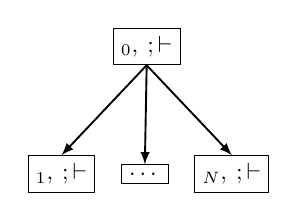
\begin{tikzpicture}[
  level distance=.75in,
  sibling distance=.15in,
  % auto,
  scale=0.85,
  edge from parent/.style={draw, thick,-latex},
  every tree node/.style={draw, align=center},
  grow'=down
]
\Tree
[.{$\sconstr_0,\:\cEnv ; \icEnv \solverRule \sconstr$}
  \edge node    { };
  [.{$\sconstr_N,\:\cEnv ; \icEnv \solverRule \sconstr$}
  ]
  \edge node[] { };
  [.{\dots}
  ]
  \edge node    { };
  [.{$\sconstr_1,\:\cEnv ; \icEnv \solverRule \sconstr$}
  ]
]
\end{tikzpicture}
& 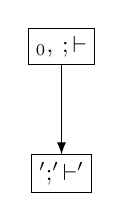
\begin{tikzpicture}[
  level distance=.75in,
  sibling distance=.15in,
  % auto,
  scale=0.85,
  edge from parent/.style={draw, thick,-latex},
  every tree node/.style={draw, align=center},
  grow'=down
]
\Tree
[.{$\sconstr_0,\:\cEnv ; \icEnv \solverRule \sconstr$}
  \edge node    { };
  [.{$\cEnv' ; \icEnv' \solverRule \sconstr'$}
  ]
]
\end{tikzpicture}
&
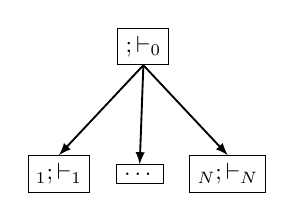
\begin{tikzpicture}[
  level distance=.75in,
  sibling distance=.15in,
  % auto,
  scale=0.85,
  edge from parent/.style={draw, thick,-latex},
  every tree node/.style={draw, align=center},
  grow'=down
]
\Tree
[.{$\emptyenv ; \icEnv \solverRule \sconstr_0$}
  \edge node    { };
  [.{$\cEnv_N; \icEnv \solverRule \sconstr_N$}
  ]
  \edge node[] { };
  [.{\dots}
  ]
  \edge node    { };
  [.{$\cEnv_1 ; \icEnv \solverRule \sconstr_1$}
  ]
]
\end{tikzpicture}
\\ & & \\ & & \\
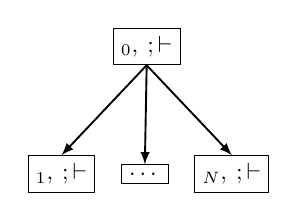
\begin{tikzpicture}[
  level distance=.75in,
  sibling distance=.15in,
  % auto,
  scale=0.85,
  edge from parent/.style={draw, thick,-latex},
  every tree node/.style={draw, align=center},
  grow'=down
]
\Tree
[.{$\sconstr_0,\:\cEnv ; \icEnv \solverRule \sconstr$}
  \edge node    { };
  [.{$\sconstr_N,\:\cEnv ; \icEnv \solverRule \sconstr$}
  ]
  \edge node[] { };
  [.{\dots}
  ]
  \edge node    { };
  [.{$\sconstr_1,\:\cEnv ; \icEnv \solverRule \sconstr$}
  ]
]
\end{tikzpicture}
& 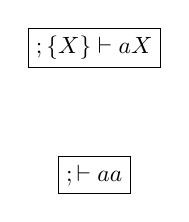
\begin{tikzpicture}[
  level distance=.75in,
  sibling distance=.15in,
  % auto,
  scale=0.85,
  edge from parent/.style={thick,-latex},
  every tree node/.style={draw, align=center},
  grow'=down
]
\Tree
[.{$\emptyenv ; \{ \csymb X \} \solverRule a \cfresh X $}
  \edge node    { };
  [.{$\emptyenv ; \icEnv \solverRule a \ceq a$}
  ]
]
\end{tikzpicture}
&
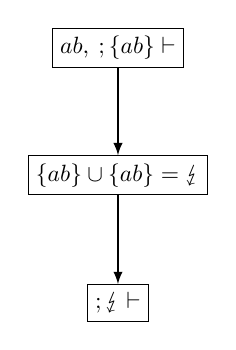
\begin{tikzpicture}[
  level distance=.75in,
  sibling distance=.15in,
  % auto,
  scale=0.85,
  edge from parent/.style={draw, thick,-latex},
  every tree node/.style={draw, align=center},
  grow'=down
]
\Tree
[.{$a \ceq b,\:\cEnv ; \{ a \cneq b \} \solverRule \sconstr$}
  \edge node    { };
  [.{$\{a \ceq b\} \cup \{ a \cneq b \} = \lightning $}
    \edge node    { };
    [.{$\cEnv ; \lightning \solverRule \sconstr$}
    ]
  ]
]
\end{tikzpicture}
\\ & & \\
\hline
    \end{tabularx}
  \caption{Base cases of the Solver's rules.}
  \label{fig:solver-base}
\end{figure}
This recursive procedure may stop at a contradictory environment $\lightning$,
which short-circuits the procedure, or at
a state in which all the assumptions and the goal itself are reduced to irreducible components,
which is then as simple as checking if the goal is trivial or if it
occurs on the left side of the turnstile.

\section{Goal-reducing rules}
We begin the description of Solver rules with the ones that break down the goal,
as we find them more straightforward to follow.
As stated previously, the actual procedure would start by reducing the assumptions
and only work on the goal when the assumption environment $\cEnv$ is empty
(all assumptions were reduced and live in the environment $\icEnv$).
These "rules" should be considered as a way to describe an algorithm
rather than a description of some inductive relation.

\begin{figure}[htbp]
    \centering
    \begin{tabularx}{\textwidth}{|C|}
      \hline \\ $
      \inference{
      }{
        \emptyenv ; \icEnv \solverRule \atomv = \atomv
      }
      \quad\;
      \inference{
      }{
        \emptyenv ; \icEnv \solverRule \termv = \termv
      }
      \quad\;
      \inference{
        \emptyenv ; \icEnv \solverRule \term_1 = \term_2
        &
        \emptyenv ; \icEnv \solverRule \term_1' = \term_2'
      }{
        \emptyenv ; \icEnv \solverRule \term_1 \term_1' = \term_2 \term_2'
      }
      $ \\ \\ $
      \inference{
        \emptyenv ; \icEnv \solverRule \atomexp_1 \cfresh \tbind{\atomexp_2}\term_2
        &
        \emptyenv ; \icEnv \solverRule \term_1 = \permswap{\atomexp_1}{\atomexp_2} \term_2
      }{
        \emptyenv ; \icEnv \solverRule \tbind{\atomexp_1} \term_1 = \tbind{\atomexp_2} \term_2
      } \qquad
      \inference{
      }{
        \emptyenv ; \icEnv \solverRule \symb = \symb
      }
      $ \\ \\ \hline
      \end{tabularx}
  \caption{Equality rules.}
  \label{fig:equality-reduction-rules}
\end{figure}
Checking equality of terms is rather straightforward and follows from the
term structure if no permutations are involved.
Only the case for abstraction terms is more complicated:
the left side's argument must be fresh in the whole right side's term
(which informally means that either the arguments are the same or
the left's argument doesn't occur at all in the right's body),
and the left body must be equal to the right body with its argument swapped for the left one.

\begin{figure}[htbp]
    \centering
    \begin{tabularx}{\textwidth}{|C|}
    \hline \\
    \begin{tabular}{ccc}
      \begin{tabular}{c} $
      \inference{
        \emptyenv ; \icEnv \solverRule \atomv = \perm^{-1} \atomexp
      }{
        \emptyenv ; \icEnv \solverRule \perm \atomv = \atomexp
      }
      $ \\ \\ $
      \inference{
        \emptyenv ; \icEnv \solverRule \termv_1 = \pi_1^{-1} \pi_2 \termv_2
      }{
        \emptyenv ; \icEnv \solverRule \pi_1 \termv_1 = \pi_2 \termv_2
      } $
      \end{tabular} & &
      \begin{tabular}{c} $
      \inference{
        \atomv \cneq \atomexp_1, \atomv \cneq \atomexp_2 ; \icEnv \solverRule \atomv     = \atomexp \\
        \atomv \ceq  \atomexp_1, \atomv \cneq \atomexp_2 ; \icEnv \solverRule \atomexp_2 = \atomexp \\
        \atomv \ceq  \atomexp_2 ; \icEnv \solverRule \atomexp_1 = \atomexp
      }{
        \emptyenv ; \icEnv \solverRule \atomv = \permswap{\atomexp_1}{\atomexp_2}{\atomexp}
      } $
      \end{tabular} \\ \\
    \end{tabular}
    \\
    \begin{tabular}{cc}
      $
      \inference{
        \emptyenv ; \icEnv \solverRule \pi \text{ idempotent on } \termv
      }{
        \emptyenv ; \icEnv \solverRule \termv = \pi \termv
      }
      $ & $
      \inference{
        \forall \atomv \in \pi.\;
          \emptyenv ; \icEnv \solverRule \atomv = \pi \atomv \;\vee\;
          \emptyenv ; \icEnv \solverRule \atomv \cfresh \termv
        }{
        \emptyenv ; \icEnv \solverRule \pi \text{ idempotent on } \termv
      }
      $ \\ & \\
    \end{tabular} \\
    \hline
    \end{tabularx}
  \caption{Permutation-reduction rules.}
  \label{fig:permutation-reduction-rules}
\end{figure}
To compare a \it{pure} atom $\atomv$ with a permuted one, we employ the decidability of atom equality
to reduce the right-hand side's permutation by applying its outermost swap $\swap{\atomexp_1}{\atomexp_2}$ on the left side's atom.
There are three possible cases: \begin{enumerate}[noitemsep]
    \item $\atomv$ is different from both $\atomexp_1$ and $\atomexp_2$,
so the swap doesn't change the goal,
    \item $\atomv$ is equal to $\atomexp_1$ but different from $\atomexp_2$,
so the swap substitutes it for $\atomexp_2$,
    \item $\atomv$ is equal to $\atomexp_2$,
so the swap substitutes it for $\atomexp_1$.
\end{enumerate}
Notice that it is impossible for any two of these assumptions to be valid at the same time\-the
contradictory branches will resolve through the absurd environment.

If the left-hand side's term is permuted, we move the permutation
to the right-hand side by inverting it.
There's also a special check for a variable equal to its permuted self\-the
only way for equality to hold is if that permutation is idempotent on it\-which
we check by taking every atom $\atomv$ from $\perm$ and checking
whether it is untouched by the permutation ($\atomv \ceq \perm \atomv$) or if it is fresh in that variable ($\atomv \cfresh \termv$).

\begin{figure}[htbp]
    \centering
    \begin{tabularx}{\textwidth}{|C|}
      \hline \\
      \begin{tabular}{ccc}
      $
      \inference{
        \atomv_1 \cneq \atomv_2 \in \icEnv
      }{
        \emptyenv ; \icEnv \solverRule \atomv_1 \cfresh \atomv_2
      }
      $ & $
      \inference{
        \atomv \cfresh \termv \in \icEnv
      }{
        \emptyenv ; \icEnv \solverRule \atomv \cfresh \termv
      }
      $ & $
      \inference{
        \csymb \termv \in \icEnv
      }{
        \emptyenv ; \icEnv \solverRule \atomv \cfresh \termv
      }
      $
      \end{tabular}
      \\ \\
      \begin{tabular}{ccc}
      $
      \inference{
        \atomv \cneq \atomexp ; \icEnv \solverRule \atomv \cfresh \term
      }{
        \emptyenv ; \icEnv \solverRule \atomv \cfresh \tbind{\atomexp}{\term}
      }
      $ &
      $
      \inference{
        \emptyenv ; \icEnv \solverRule \atomv \cfresh \term_1
        &
        \emptyenv ; \icEnv \solverRule \atomv \cfresh \term_2
      }{
        \emptyenv ; \icEnv \solverRule \atomv \cfresh \term_1 \term_2
      }
      $ & $
      \inference{
      }{
        \emptyenv ; \icEnv \solverRule \atomv \cfresh \symb
      }
      $
      \end{tabular}
      \\ \\ \hline
      \end{tabularx}
  \caption{Freshness rules.}
  \label{fig:freshness-rules}
\end{figure}
Freshness follows the term structure and breaks down into an assumption check or a trivial case.
Unlike how we defined freshness in abstraction in the introduction,
we do not have two rules that differ based on whether $\atomv \ceq \atomexp$.
If they are indeed equal, then the assumption of inequality will immediately
result in a contradiction of the environment, but if it wasn't yet established,
then we continue the solver procedure with an additional assumption.

\begin{figure}[htbp]
    \centering
    \begin{tabularx}{\textwidth}{|CC|}
      \hline & \\ $
      \inference{
      }{
        \emptyenv ; \icEnv \solverRule \shatom \csheq \shatom
      }
      $ & $
      \inference{
      }{
        \emptyenv ; \icEnv \solverRule \symb \csheq \symb
      }
      $ \\ & \\
      $
      \inference{
        \termv_1 \csheq \termv_2 \in \icEnv
      }{
        \emptyenv ; \icEnv \solverRule \termv_1 \csheq \termv_2
      }
      $ & $
      \inference{
        \termv  \csheq \shape' \in \icEnv
        &
        \emptyenv ; \icEnv \solverRule \shape'  \csheq \shape
      }{
        \emptyenv ; \icEnv \solverRule \termv  \csheq \shape
      }
      $ \\ & \\
      $\inference{
        \emptyenv ; \icEnv \solverRule \shape_1 \csheq \shape_2
      }{
        \emptyenv ; \icEnv \solverRule \shbind \shape_1 \csheq \shbind \shape_2
      }
      $ & $
      \inference{
        \emptyenv ; \icEnv \solverRule \shape_1 \csheq \shape_2
        &
        \emptyenv ; \icEnv \solverRule \shape_1' \csheq \shape_2'
      }{
        \emptyenv ; \icEnv \solverRule \shape_1 \shape_1' \csheq \shape_2 \shape_2'
      }
      $ \\ & \\ $
      \inference{
        \emptyenv ; \icEnv \solverRule \shape_1 \csheq \shape_2
        &
        \shape_2 \cshlt \termv \in \icEnv
      }{
        \emptyenv ; \icEnv \solverRule \shape_1 \cshlt \termv
      }
      $ & $
      \inference{
        \emptyenv ; \icEnv \solverRule \shape_1 \cshlt \shape_2
        &
        \shape_2 \cshlt \termv \in \icEnv
      }{
        \emptyenv ; \icEnv \solverRule \shape_1 \cshlt \termv
      }
      $ \\ & \\ \hline
      \end{tabularx}
  \caption{Shape and subshape rules.}
  \label{fig:shape-rules}
\end{figure}
Shape equality is naturally structural.
All atoms are considered to have the same shape, while
variables can share shapes and have their shape stored by $\icEnv$,
which enables transitivity.
Solving subshape recurses through the right-hand side shape's structure to find a shape-equal sub-shape.
Otherwise, we use assumptions in environment $\icEnv$ to identify all shapes that given variable subshapes.

\begin{figure}[htbp]
    \centering
    \begin{tabularx}{\textwidth}{|CCC|}
      \hline & & \\ $
      \inference{
      }{
        \emptyenv ; \icEnv \solverRule \csymb \symb
      }
      $ & $
      \inference{
        \csymb \termv \in \icEnv
      }{
        \emptyenv ; \icEnv \solverRule \csymb \termv
      }
      $ & $
      \inference{
        \csymb \termv \in \icEnv
      }{
        \emptyenv ; \icEnv \solverRule \atomv \cfresh \termv
      }
      $ \\ & & \\ \hline
      \end{tabularx}
  \caption{Symbol rules.}
  \label{fig:symbol-rules}
\end{figure}
Symbol constraints are really simple to check; it can either be that the term is already
a symbol, or it is a variable that we assumed to be some symbol.

\section{Assumption-reducing rules}
But before the Solver can reduce the goal-constraint, it must first reduce all assumptions in the $\cEnv$ environment.
We will now present the rules for reducing the constraints on the left side of the turnstile,
which are mostly analogous to the goal-reducing rules.

\begin{figure}[htpb]
  \centering
  \begin{tabularx}{\textwidth}{|C|}
  \hline \\
  \begin{tabular}{ccc} $
    \inference{
      \atomexp_1 \cfresh \tbind{\atomexp_2} \term_2\:,\;
        \term_1 = \permswap{\atomexp_1}{\atomexp_2}\term_2 \:, \;
        \cEnv ; \icEnv \solverRule \sconstr
    }{
      \tbind{\atomexp_1} \term_1 \ceq \tbind{\atomexp_2} \term_2 , \cEnv ; \icEnv \solverRule \sconstr
    } $ & & $
    \inference{
      \atomv \ceq \atomexp, \; \cEnv ; \icEnv \solverRule \sconstr
      \\
      \atomv \cneq \atomexp, \; \atomv \cfresh \term,\;\cEnv ; \icEnv \solverRule \sconstr
    }{
      \atomv \cfresh \tbind{\atomexp} \term , \cEnv ; \icEnv \solverRule \sconstr
    } $
  \end{tabular}
  \\ \\
  \begin{tabular}{ccc} $
    \inference{
      \atomv \cneq \atomexp_1, \atomv \cneq \atomexp_2, \atomv     \ceq \atomexp, \cEnv ; \icEnv \vDash \sconstr \\
      \atomv \ceq  \atomexp_1, \atomv \cneq \atomexp_2, \atomexp_2 \ceq \atomexp, \cEnv ; \icEnv \vDash \sconstr \\
                              \atomv \ceq  \atomexp_2, \atomexp_1 \ceq \atomexp, \cEnv ; \icEnv \vDash \sconstr
    }{
      \atomv \ceq \permswap{\atomexp_1}{\atomexp_2} \atomexp, \cEnv ; \icEnv \vDash \sconstr
    } $ & & $
    \inference{
      \atomv \cneq \atomexp_1, \atomv \cneq \atomexp_2, \atomv     \cfresh \perm\termv, \cEnv ; \icEnv \vDash \sconstr \\
      \atomv \ceq  \atomexp_1, \atomv \cneq \atomexp_2, \atomexp_2 \cfresh \perm\termv, \cEnv ; \icEnv \vDash \sconstr \\
                              \atomv \ceq  \atomexp_2, \atomexp_1 \cfresh \perm\termv, \cEnv ; \icEnv \vDash \sconstr
    }{
      \atomv \cfresh \permswap{\atomexp_1}{\atomexp_2} \perm\termv, \cEnv ; \icEnv \vDash \sconstr
    } $
  \end{tabular}
  \\ \\\hline
  \end{tabularx}
  \caption{Selected equality and freshness assumption-reducing rules.}
  \label{fig:abstraction}
\end{figure}
Again, the binding term constructor is of most interest to us:
equality behaves the same as on the goal side; we simply
split up the assumption into two assumptions the same way we would split the goal.
For freshness of an atom in an abstraction, we consider two cases:
either the atom is equal to the argument,
or different from the argument but fresh in the body.
In contrast to the goal-reducing rules where we would be satisfied with
just one branch succeeding, here we expect both possibilities to be satisfiable.
To deal with atom swapping and freshness within the presence of a permutation,
we reduce the atom by considering the swap cases, analogous to how we did in the
goal-reducing assumptions.

\begin{figure}[htbp]
  \centering
  \framebox[\textwidth]{
    \begin{tabularx}{\textwidth}{Cr}
      \\ $
      \inference{
        \termv = \pi^{-1} \term, \cEnv ; \icEnv \solverRule \sconstr
      }{
        \pi \termv = \term, \cEnv ; \icEnv \solverRule \sconstr
      }
      \qquad
      \inference{
        \atomv \ceq \pi^{-1} \atomexp, \cEnv ; \icEnv \solverRule \sconstr
      }{
        \pi \atomv \ceq \atomexp, \cEnv ; \icEnv \solverRule \sconstr
      } $ \\ \\ $
      \inference{
        \pi \text{ idempotent on } \termv, \cEnv ; \icEnv \solverRule \sconstr
      }{
        \termv = \pi \termv, \cEnv ; \icEnv \solverRule \sconstr
      } \qquad
      \inference{
        \emptyenv ; \icEnv \solverRule \text{ idempotent on } \termv
        &
        \cEnv ; \icEnv \solverRule \sconstr
      }{
        \pi \text{ idempotent on } \termv, \cEnv ; \icEnv \solverRule \sconstr
      } $ \\ \\ $
      \inference{
        (\forall \atomv \in \pi.\;\atomv = \pi \atomv \;\vee\;\atomv \cfresh \termv), \cEnv ; \icEnv \solverRule \sconstr
      }{
        \pi \text{ idempotent on } \termv, \cEnv ; \icEnv \solverRule \sconstr
      } $ \\ \\
    \end{tabularx}
  }
  \caption{Permutation-reducing rules.}
  \label{fig:perm-reduction}
\end{figure}
We first deal with the left-hand side's permutation by inverting it and moving it to the right-hand side.
Otherwise, both equality and freshness assumptions follow from the term structure.
We again must consider the special case where a variable is assumed to be equal to itself with some permutation applied, where we extend the environment $\cEnv$ by a meta-assumption denoted as
$(\forall \atomv \in \perm.\;\atomv = \perm \apperm \atomv \;\vee\;\atomv \cfresh \termv)$.
The Solver handles this by creating multiple environments where each atom $\atomv$ occurring in the permutation $\perm$ generates an assumption $\atomv = \pi \atomv$ or $\atomv \cfresh \termv$, and every combination of these assumptions is used to create new environments by
adding them to the environment $\cEnv$, which are then used to run the Solver on the same goal.

While the assumption of the permutation being idempotent might appear to multiply the number of assumptions exponentially based on the number of atoms in the given permutation,
it's worth noting that this number is unlikely to be very high, as permutations rarely consist of more than a few swaps.
In practice, the solver implementation will initially check whether the permutation is idempotent with an empty set of assumptions.
Only if this initial check fails, will it proceed to examine the permutation atom by atom.

\begin{figure}[hbtp]
  \centering
  \begin{tabularx}{\textwidth}{|C|}
      \hline \\ $
      \inference{
        \cEnv\subst{\termv}{\term} ; \icEnv\subst{\termv}{\term}
          \solverRule \sconstr\subst{\termv}{\term}
      }{
        \termv = \term, \cEnv ; \icEnv \solverRule \sconstr
      % }\:\scbrk{Subst}{Term}$ \\ \\
      }$ \\ \\
      $
      \inference{
        \cEnv \subst{\atomv_1}{\atomv_2}; \icEnv\subst{\atomv_1}{\atomv_2}
          \solverRule \sconstr\subst{\atomv_1}{\atomv_2}
      }{
        \atomv_1 \ceq \atomv_2, \cEnv ; \icEnv \solverRule \sconstr
      % }\:\scbrk{Subst}{Atom}$ \\
      }$ \\
    \begin{tabular}{cc}
    & \\ $
    \inference{
      \cEnv ; \{\atomv_1 \cneq \atomv_2\} \cup \icEnv \solverRule \sconstr
    }{
      \atomv_1 \cneq \atomv_2, \; \cEnv ; \icEnv \solverRule \sconstr
    }
    $ & $
    \inference{
      \cEnv ; \{\atomv \cfresh \termv\} \cup \icEnv \solverRule \sconstr
    }{
      \atomv \cfresh \termv, \; \cEnv ; \icEnv \solverRule \sconstr
    }
    $ \\ & \\ $
    \inference{
      \cEnv ; \{\termv_1 \csheq \termv_2\} \cup \icEnv \vDash \sconstr
    }{
      \termv_1 \csheq \termv_2, \cEnv ; \icEnv \vDash \sconstr
    }
    $ & $
    \inference{
      \cEnv ; \{\termv \csheq \shape\} \cup \icEnv \vDash \sconstr
    }{
      \termv \csheq \shape,\; \cEnv ; \icEnv \vDash \sconstr
    }
    \quad
    $ \\ & \\ $
    \inference{
      \cEnv ; \{\term \cshlt \termv\} \cup \icEnv \vDash \sconstr
    }{
      \term \cshlt \termv, \cEnv ; \icEnv \vDash \sconstr
    }
    $ & $
    \inference{
      \cEnv ; \{\csymb \termv\} \cup \icEnv \vDash \sconstr
    }{
      \csymb \termv, \cEnv ; \icEnv \vDash \sconstr
    }
    $ \\ & \\
    \end{tabular}
    \\ \hline
    \end{tabularx}
  \caption{Rules dealing with irreducible assumptions.}
  \label{fig:assumption-equality-rules}
\end{figure}
In the end, all assumptions reach the irreducible components that are handled through
the special environment $\icEnv$.
Equality assumptions reduce to the substitution of the name for the expression, where
substituting in the $\icEnv$ environment is a more involved process
that can lead to a contradiction or extract assumptions from $\icEnv$ back into $\cEnv$.
Otherwise, assumptions are simply moved to the environment of irreducible
constraints via a procedure that we describe in the next section.

Before delving into further details, we present an example showcasing the Solver in action, as depicted in figure \ref{fig:solver-example} on the next page.
We will see how it decides that the assumed constraints $(a \cneq b,\: a \cneq c,\: b \cfresh \tbind{a}\permswap{b}{c}{E})$
collectively imply the satisfaction of the goal constraint $(c \cfresh E)$
by performing a procedure resembling an exhaustive search on atom comparison.

It begins by taking the already irreducible assumptions $(a \cneq b,\: a \cneq c)$ and moving them to $\icEnv$.
Then, it analyzes how $b \cfresh \tbind{a}\permswap{b}{c}{E}$
can hold, branching into two possibilities.
The first case is that $b$ and $a$ are equal and quickly leads to contradiction.
The second one is that $b$ is different from $a$ and fresh in $\permswap{b}{c}{E}$.
To deal with freshness, the Solver must reduce the swap $\permswap{b}{c}$ on $E$,
prompting further branching by comparing $b$ with the atoms in the swap.
The first case is that $b$ is neither $b$ nor $c$, contradicting the reflexivity of equality.
The second one is that $b$ is equal to $b$ but different from $c$, so it gets swapped for $c$
in the freshness assumption, which then becomes $c \cfresh E$ and matches with the goal.
The final case is that $b$ is equal to $c$, so the Solver merges these atoms together,
substituting $b$ with $c$ everywhere.
The freshness assumption turns into $c \cfresh E$ by substitution, so it again matches the goal.
As all branches resolved properly, the whole judgment is proved.

% $0.\quad a \cneq b,\: a \cneq c,\: b \cfresh \tbind{a}\permswap{b}{c}{E} \:;\; \emptyenv \solverRule c \cfresh E $
% $0'.\quad b \cfresh \tbind{a}\permswap{b}{c}{E} \:;\; \{a \cneq b,\: a \cneq c\} \solverRule c \cfresh E $ \\
% $1.\quad b \ceq a \:;\; \{a \cneq b,\: a \cneq c\} \solverRule c \cfresh E $ \\
% $1'.\quad (b \cneq a) \in \{a \cneq b,\: a \cneq c\}$
% $2.\quad b \cneq a,\: b \cfresh \permswap{b}{c}{E} \:;\; \{a \cneq b,\: a \cneq c\}\solverRule c \cfresh E $
% $2'.\quad b \cfresh \permswap{b}{c}{E} \:;\; \{a \cneq b,\: a \cneq c\}\solverRule c \cfresh E $ \\
% $2.1 \quad b \cneq b,\: b \cneq c,\: b \cfresh E \:;\; \{a \cneq b,\: a \cneq c\}\solverRule c \cfresh E $ \\
% $2.1' \quad \{b \cneq b\} \cup \{a \cneq b,\: a \cneq c\} = \lightning $ \\
% $2.2 \quad b \ceq b,\: b \cneq c,\: c \cfresh E \:;\; \{a \cneq b,\: a \cneq c\} \solverRule c \cfresh E $ \\
% $2.2' \quad b \cneq c,\: c \cfresh E \:;\; \{a \cneq b,\: a \cneq c\} \solverRule c \cfresh E $ \\
% $2.2'' \quad c \cfresh E \:;\; \{a \cneq b,\: a \cneq c,\: b \cneq c\} \solverRule c \cfresh E $ \\
% $2.2''' \quad \emptyenv\:;\; \{a \cneq b,\: a \cneq c,\: b \cneq c,\: c \cfresh E \} \solverRule c \cfresh E $ \\
% $2.2'''' \quad \{c \cfresh E\} \in \{a \cneq b,\: a \cneq c,\: b \cneq c,\: c \cfresh E \} $ \\
% $2.3 \quad b \ceq c,\: b \cfresh E \:;\; \{a \cneq b,\: a \cneq c\} \solverRule c \cfresh E $ \\
% $2.3' \quad c \cfresh E \:;\; \{a \cneq c \} \solverRule c \cfresh E $ \\
% $2.3'' \quad \emptyenv \:;\; \{a \cneq c,\: c \cfresh E \} \solverRule c \cfresh E $ \\
% $2.3''' \quad \{c \cfresh E\} \in \{a \cneq c,\: c \cfresh E \} $ \\
%
\begin{figure}[htpb]
\centering
\rotatebox{90}{
\begin{tikzpicture}[
  level distance=.75in,
  sibling distance=.15in,
  % auto,
  scale=0.85,
  edge from parent/.style={draw, thick,-latex},
  every tree node/.style={draw, align=center},
  grow'=down
]
\Tree
[.{$a \cneq b,\: a \cneq c,\: b \cfresh \tbind{a}\permswap{b}{c}{E} \:;\; \emptyenv \solverRule c \cfresh E$}
  \edge node    { };
  [.{$b \cfresh \tbind{a}\permswap{b}{c}{E} \:;\; \{a \cneq b,\: a \cneq c\} \solverRule c \cfresh E$}
    \edge node { };
    [.{$b \cneq a,\: b \cfresh \permswap{b}{c}{E} \:;\; \{a \cneq b,\: a \cneq c\}\solverRule c \cfresh E$}
    \edge node { };
    [.{$b \cfresh \permswap{b}{c}{E} \:;\; \{a \cneq b,\: a \cneq c\}\solverRule c \cfresh E$}
    \edge node { };
    [.{$b \ceq c,\: b \cfresh E \:;\; \{a \cneq b,\: a \cneq c\} \solverRule c \cfresh E$}
    \edge node { };
    [.{$c \cfresh E \:;\; \{a \cneq c \} \solverRule c \cfresh E$}
    \edge node { };
    [.{$\emptyenv \:;\; \{a \cneq c,\: c \cfresh E \} \solverRule c \cfresh E$}
    \edge node { };
    [.{$(c \cfresh E) \in \{a \cneq c,\: c \cfresh E \}$} ]
    ]
    ]
    ]
    \edge node { };
    [.{$b \ceq b,\: b \cneq c,\: c \cfresh E \:;\; \{a \cneq b,\: a \cneq c\} \solverRule c \cfresh E$}
    \edge node { };
    [.{$b \cneq c,\: c \cfresh E \:;\; \{a \cneq b,\: a \cneq c\} \solverRule c \cfresh E$}
    \edge node { };
    [.{$c \cfresh E \:;\; \{a \cneq b,\: a \cneq c,\: b \cneq c\} \solverRule c \cfresh E$}
    \edge node { };
    [.{$\emptyenv\:;\; \{a \cneq b,\: a \cneq c,\: b \cneq c,\: c \cfresh E \} \solverRule c \cfresh E$}
    \edge node { };
    [.{$(c \cfresh E) \in \{a \cneq b,\: a \cneq c,\: b \cneq c,\: c \cfresh E \}$} ]
    ]
    ]
    ]
    ]
    \edge node { };
    [.{$b \cneq b,\: b \cneq c,\: b \cfresh E \:;\; \{a \cneq b,\: a \cneq c\}\solverRule c \cfresh E$}
    \edge node { };
    [.{$\{b \cneq b\} \cup \{a \cneq b,\: a \cneq c\} = \lightning$} ]
    ]
    ]
    ]
    \edge node { };
    [.{$b \ceq a \:;\; \{a \cneq b,\: a \cneq c\} \solverRule c \cfresh E$}
    \edge node { };
    [.{$\{b \ceq a\} \cup \{a \cneq b,\: a \cneq c\} = \lightning$} ]
    ]
    ]
  ]
]
\end{tikzpicture}
}
\caption{Example of running Solver.}
\label{fig:solver-example}
\end{figure}

\newpage

\section{Irreducible constraints} \label{sec:solverenv}
Environment $\icEnv$ that contains all the irreducible assumptions is given by
a sextuple
$(\NeqAtoms_{\icEnv}
, \Fresh_{\icEnv}
, \VarShape_{\icEnv}
, \Shape_{\icEnv}
, \Subshape_{\icEnv}
, \Symbols_{\icEnv}
)$.
\begin{figure}[h]
  \begin{tabularx}{\textwidth}{|l|X|}
  \hline
    $\NeqAtoms$ & Set of pairs of atoms that are known to be different. \\
  \hline
    $\Fresh$ & Set of pairs of atom and variable, indicating that the atom is \it{fresh} in the variable. \\
  \hline
    $\VarShape$ & Mapping from variables to shape-representative variables. All variables mapped to the same representative are considered to inhabit the same shape. \\
  \hline
    $\Shape$ & Mapping from shape-representative variables to the actual shape it must inhabit. \\
  \hline
    $\Subshape$ & Set of pairs of shape-representative variables and shapes that subshape the variable. \\
  \hline
    $\Symbols$ & Set of shape-representative variables that are known to be some unknown functional symbols. \\
  \hline
  \end{tabularx}
  \caption{Description of environment $\icEnv$.}
  \label{fig:assumption-equality-rules}
\end{figure}

\begin{figure}[htbp]
  \begin{mdframed}
  \centering
    \begin{tabular}{p{0.55\textwidth}p{0.39\textwidth}}
      \begin{lstlisting}[mathescape,language=OCaml]
    $\shrep{\termv} :=$
      | if $Y$ $\leftarrow\;$var_shape$_\icEnv$ $\termv$ then $\shrep{Y}$
      | otherwise $\termv$

    $\shenv{\termv} :=$
      | if $Y$ $\leftarrow\;$var_shape$_\icEnv$ $\termv$ then $\shenv{Y}$
      | if $\shape$ $\leftarrow\;$shape$_\icEnv$ $\termv$ then $\shape$
      | otherwise $\termv$
      \end{lstlisting}
      &
      \begin{lstlisting}[mathescape,language=OCaml]


  $\shenv{\shatom}        \:$  $\:\:\; :=$ $\shatom $
  $\shenv{\shbind \shape} \:$  $:=$ $\shbind \shenv{\shape} $
  $\shenv{\shape_1 \shape_2}\;$ $:=$ $\shenv{\shape_1} \shenv{\shape_2}$
  $\shenv{\symb}           \;$   $:=$ $\symb $
      \end{lstlisting}
    \end{tabular}
    \\[-4ex]
    \begin{tabular}{rcl}
      $(\atomv_1 \cneq \atomv_2)  \in \icEnv $ & $:=$ & $ (\atomv_1 \cneq \atomv_2) \in \NeqAtoms_{\icEnv} $ \\
      $(\atomv \cfresh \termv)    \in \icEnv $ & $:=$ & $ \termv \in \Fresh_{\icEnv}(\atomv) $ \\
      $(\termv_1 \csheq \termv_2) \in \icEnv $ & $:=$ & $ \shenv{\termv_1} \ceq \shenv{\termv_2} $ \\
      $(\termv \csheq \shape)     \in \icEnv $ & $:=$ & $ \shape = \Shape_{\icEnv}(\shrep{\termv})$ \\
      $(\shape \cshlt \termv)     \in \icEnv $ & $:=$ & $ \shape \in \Subshape_{\icEnv}(\shrep{\termv})$ \\
    \\
    \end{tabular}
  \end{mdframed}
  \caption{Interpretation of shapes and assumptions in $\icEnv$.}
  \label{fig:interpretation}
\end{figure}
With such environment structure, we now establish a method to compute the shape-representative variable and
outline the procedure for reconstructing the shape within the environment $\icEnv$,
denoted \shenv{\shape}.
Verifying whether a constraint is included in $\icEnv$ can then be accomplished straightforwardly.

% \pagebreak

\begin{figure}[hbtp]
  \centering
  \framebox[\textwidth]{
    \begin{tabularx}{\textwidth}{c}
    \\ $
    \;
    \inference{
      \stxoccurs{\shrep{\termv}}{\shenv{\shape}}
    }{
      \icEnv \solverRule \occurs{\termv}{\shape}
    }
    \quad\;
    \inference{
      \stxoccurs{\termv'}{\shenv{\shape}}
      \\
        (\shape' \cshlt \termv') \in \icEnv
        &
        \icEnv \solverRule \occurs{\termv}{\shape'}
    }{
      \icEnv \solverRule \occurs{\termv}{\shape}
    }
    $ \\ \\
    \end{tabularx}
  }
  \caption{Occurs check rules.}
  \label{fig:subkinding-rules}
\end{figure}
Additionally, we establish rules for a~special occurs check procedure,
which safeguards against handling circular references,
and does so while considering all occurrences in the assumptions of $\icEnv$.
This is needed because of the shape assumptions we introduced;
we must go with the occurrence check through the ``shape-similar'' variables and shapes.

To describe the procedures handling environment $\icEnv$, we use OCaml's pipelining notation of << \lstinline[mathescape,language=OCaml]{x |> f1 |> ... |> fn} >>
for  << \lstinline[mathescape,language=OCaml]{fn (... (f1 x))} >>
and abuse notation like << \lstinline[mathescape,language=OCaml]{fresh += x} >>
for functions <<
\lstinline[mathescape,language=OCaml] {fun $\icEnv$ -> $\{\icEnv$ with fresh = x :: $\icEnv$.fresh$\}$}
>>.
\begin{figure}[htbp]
    \begin{tabular}{|p{0.95\textwidth}|}
        \hline
        \begin{tabular}{ll}
      \begin{lstlisting}[mathescape,language=OCaml]
   $\{\atomv \cfresh \termv\} \cup \icEnv :=$
     $\icEnv\;$ |> fresh += ($\atomv \cfresh \termv$)
\end{lstlisting}
&
 \begin{lstlisting}[mathescape,language=OCaml]

$\{\atomv \cneq \atomv'\} \cup \icEnv :=$
  | if $\atomv \ceq \atomv'$ then $\lightning$
  | otherwise $\icEnv\;$|> neq_atoms += ($\atomv \cneq \atomv'$)
\end{lstlisting}
\end{tabular} \\
\begin{lstlisting}[mathescape,language=OCaml]
    $\{\termv \csheq \shape\} \cup \icEnv :=$
      | if $\occurs{\shrep{\termv}}{\shenv{\shape}}$ then $\lightning$
      | otherwise $\icEnv\;$|> symbols  $\{\shrep{\termv} \leadsto \shenv{\shape}\}$
                    |> subshape $\{\shrep{\termv} \leadsto \shenv{\shape}\}$
                    |> shape    $\{\shrep{\termv} \leadsto \shenv{\shape}\}$

    $\{\termv \csheq \termv'\} \cup \icEnv :=$
      | if $\shrep{\termv} \ceq \shrep{\termv'}$ then $\icEnv$
      | if $\shenv{\termv} \ceq \shenv{\termv'}$ then $\icEnv$
      | if $\occurs{\shrep{\termv}}{\shenv{\termv'}}$ then $\lightning$
      | if $\occurs{\shrep{\termv'}}{\shenv{\termv}}$ then $\lightning$
      | otherwise $\icEnv\;$|> symbols        $\{\shrep{\termv} \leadsto \shrep{\termv'}\}$
                    |> subshape       $\{\shrep{\termv} \leadsto \shrep{\termv'}\}$
                    |> transfer_shape $\{\shrep{\termv} \leadsto \shrep{\termv'}\}$
                    |> var_shape += $(\shrep\termv \mapsto \shrep\termv')$
                    |> shape     -= $\shrep\termv$
                    |> subshape  -= $\shrep\termv$
\end{lstlisting} \\
      \hline
    \end{tabular}
  \caption{Adding constraints to $\icEnv$.}
  \label{fig:adding-constraints}
\end{figure}
% To maintain a high-level description, we delegate the detailed implementation aspects to auxiliary functions responsible for substituting shape-variables within the given field of $\icEnv$.
Incorporating atom constraints into $\icEnv$ proceeds as follows:
freshness of an atom in a variable is simply acknowledged in the $\Fresh$ mapping.
Inequality of two atoms adds them to the set $\NeqAtoms$,
unless invoked with identical atoms, in which case we report a contradiction.
To set variable shape, we first make sure to perform an occurs check on the proposed shape
and then substitute the shape-variable in all affected fields.
To meld together two shape-variables, we first check whether they have already been merged.
If they have, we return a contradiction.
Next, we conduct an occurs check to ensure that merging them won't create a circular reference. If this check fails, we again report a contradiction.
Finally, we merge all the information pertaining to $\termv$ into $\termv'$ and
remove any traces of $\termv$ from within the $\icEnv$ environment.

\begin{figure}[htbp]
    \begin{tabular}{|p{0.95\textwidth}|}
        \hline
      \begin{lstlisting}[mathescape,language=OCaml]
    $\icEnv$ $\{\termv \mapsto \term\}$ $:=$
      $\icEnv\;$|> fresh -= $\termv$
        |> assumptions += $(\termv \csheq \shenv{\term})$
        |> assumptions += $\bigcup_{(\atomv \cfresh \termv) \in \icEnv} (\atomv \cfresh \term)$

    $\icEnv$ $\{\atomv \mapsto \atomv'\}$ $:=$
      $\icEnv\;$|> fresh -= $\atomv$
        |> fresh += $(\atomv' \cfresh{}$fresh$_\icEnv$$\atomv)$
        |> clear neq_atoms
        |> assumptions += $\bigcup_{(\atomv_1 \cneq \atomv_2) \in \icEnv} (\atomv_1\{\atomv \mapsto \atomv'\} \cneq \atomv_2\{\atomv \mapsto \atomv'\})$
\end{lstlisting} \\
      \hline
    \end{tabular}
  \caption{Substitution in $\icEnv$.}
  \label{fig:substitution}
\end{figure}
Finally, we demonstrate how the substitution of variables and atoms is accomplished,
thereby concluding the description of the \it{Solver} and its environment.
Note that we are using the meta-field of $\Assumptions$ to indicate that some of the
assumptions in $\icEnv$ are no longer "simple" and escape from $\icEnv$ back to
$\cEnv$ to be broken up by the \it{Solver}.
\begin{figure}[hbtp]
    \begin{tabular}{|p{0.95\textwidth}|}
        \hline
      \begin{lstlisting}[mathescape,language=OCaml]
    symbols $\{\termv \leadsto \shape\}$ $\icEnv$ $:=$
      | if $\shrep{\termv} \notin$ symbols$_\icEnv$ then $\icEnv$
      | otherwise $\icEnv\;$|> symbols -= $\termv$
                    |> assumptions += ($\textnormal{symbol } \shape$)

    shape $\{\termv \leadsto \shape\}$ $\icEnv$ $:=$
      | if $\shape' \leftarrow\;$shape$_\icEnv$ $\termv$ then $\icEnv$ |> assumptions += $(\shape \csheq \shape')$
      | otherwise $\icEnv\;$|> shapes += $(\termv \mapsto \shape)$

    subshape $\{\termv \leadsto \shape\}$ $\icEnv$ $:=$
      $\icEnv\;$|> assumptions += $($subshapes$_\icEnv \termv \cshlt \shape)$

    transfer_shape $\{\termv \leadsto \termv'\}$ $\icEnv$ $:=$
      | if $\shape \leftarrow\;$shape$_\icEnv$ $\termv$ then $\icEnv$ |> shape $\{\termv' \leadsto \shape\}$
      | otherwise $\icEnv$
\end{lstlisting} \\
      \hline
    \end{tabular}
  \caption{Auxiliary functions in $\icEnv$.}
  \label{fig:solverenv-auxiliary}
\end{figure}

The curious reader should now feel obliged to ask themselves a very important question:
does the Solver's procedure always stop?

To address this question, we define the state of the Solver as a triple $(\cEnv, \icEnv, \sconstr)$.
Upon analyzing the Solver rules, it becomes evident that each rule consistently
leads to a lesser state by reducing it through one or more of the following actions:
\begin{enumerate}[noitemsep]
  \item Decreasing the number of distinct variables in $\cEnv$, $\icEnv$, and $\sconstr$,
  or maintaining the same number while:
  \item Decreasing the depth of $\sconstr$,
  or preserving the current depth while:
  \item Reducing assumptions with a given depth in either $\cEnv$ or $\icEnv$ into assumptions with lower depth,
  or maintaining the number and depth of assumptions, while:
  \item Eliminating an assumption from $\cEnv$ and introducing an assumption of the same depth into $\icEnv$.
\end{enumerate}

That concludes the definition of the Solver.
In the following chapters, when we write $\cEnv \vDash \constr$,
we actually mean $\cEnv ; \varnothing\solverRule \sconstr$.
This equivalence is established by the construction of $\solverRule$,
which aligns with the interpretation of $\vDash$ as defined in the model.

%%%%%%%%%%%%%%%%%%%%%%%%%%%%%%%%%%%%%%%%%%%%%%%%%%%%%%%%%%%%%%%%%%%%%%%%%%%%%%%%
\chapter{Higher-Order Logic}
By constructing the Solver, we have built a sound logical system designed for handling and resolving constraints.
We will now extend its utility and accessibility
by introducing a higher-order logic layered atop the sublogic of constraints.
This logical framework includes all essential elements necessary for
formalizing theories, such as traditional connectives and quantifiers,
functions and relations, and special formulae that have constraints embedded inside them,
providing a versatile platform for expressing and reasoning about syntactic properties.

The Solver's decidable procedure allows us to integrate
it with the very core of our logic to enhance its capabilities
by reasoning about constraints.
In the subsequent chapter, we will see how the Solver lets us
treat constraints as propositions,
ensures that constraints guarding formulas are satisfied,
and enables us to express safe recursive predicates through the fixpoint operator.

Next, our focus will shift towards constructing a dedicated proof system for this higher-order logic, including a proof assistant.
Binding together all these components creates a cohesive framework
for precise articulation and reasoning of complex syntactic properties.


%%%%%%%%%%%%%%%%%%%%%%%%%%%%%%%%%%%%%%%%%%%%%%%%%%%%%%%%%%%%%%%%%%%%%%%%%%%%%%%
\section{Kinds}
To organize the different types of formulas within this logic, we introduce the concept of \it{kinds}.
The kind checker ensures that the formulas under consideration are coherent, given the multiple ways atoms, terms, binders, and constraints may appear within them. This step is essential for maintaining the logical integrity and meaningful interpretation of the formulas.
\begin{figure}[htbp]
  \framebox[\textwidth]{
\begin{tabularx}{\textwidth}{rcl@{\extracolsep{\fill}}r}
$\kind$ & $::=$ & $\kProp
            \bnfor \kind \karrow \kind
            \bnfor \kForallAtom{\atomv} \kind
            \bnfor \kForallTerm{\termv} \kind
            \bnfor \kGuard{\constr} \kind$
    & (kinds) \\
\end{tabularx}
  }
  \caption{Syntax of kinds.}
  \label{fig:kinds-grammar}
\end{figure}

\begin{figure}[htbp]
\begin{tabularx}{\textwidth}{|l|X|}
\hline
$\formphi \ofkind \kProp$ & $\formphi$ is a propositional formula.
\\ \hline
$\formphi \ofkind \kind_1 \karrow \kind_2$ & \makecell[l]{$\formphi$ is a function that takes a formula of kind $\kind_1$, \\ and produces a formula of kind $\kind_2$.}
\\ \hline
$\formphi \ofkind \kForallAtom{\atomv} \kind$ & \makecell[l]{$\formphi$ is a function that takes an atom expression, binds it to $\atomv$, \\ and produces a formula of kind $\kind$.}
\\ \hline
$\formphi \ofkind \kForallTerm{\termv} \kind$ & \makecell[l]{$\formphi$ is a function that takes a term, binds it to $\termv$, \\ and produces a formula of kind $\kind$.}
\\ \hline
$\formphi \ofkind \kGuard{\constr} \kind$ & \makecell[l]{$\formphi$ is a formula of kind $\kind$ as long as $\constr$ is satisfied.}
\\ \hline
\end{tabularx}
  \caption{Semantics of kinds.}
  \label{fig:kinds-semantics}
\end{figure}
Notice that as constraints occur in kinds, we cannot simply give functions
from atoms some kind ${Atom}\karrow\kind$, but we must know \it{which} atom
is bound there, to substitute for it in its kind $\kind$\-the same way we substitute
that atom for an atom expression in the function body when applying it to the formula.
The \it{guarded kind} $\kGuard{\constr} \kind$ is most importantly used in
kinding of the fixpoint formulas, which we will explain in later sections.

\section{Subkinding}
\begin{figure}[htbp]
  \centering
    \begin{tabular}{|c|}
        \hline \\
        \begin{tabularx}{\textwidth}{ccC} { } &
        $\inference{
        }{
          \cEnv \vdash \kind \subkind \kind
        }\:\scbrk{Subkind}{Refl}
        $ & $
        \inference{
          \cEnv \vdash \kind_1 \subkind \kind_2 &
          \cEnv \vdash \kind_2 \subkind \kind_3
        }{
          \cEnv \vdash \kind_1 \subkind \kind_3
        }\:\scbrk{Subkind}{Trans} $ \\
        \end{tabularx} \\ \\
        $\inference{
          \cEnv \vdash \kind_1 \subkind \kind_2
        }{
          \cEnv \vdash \kForallAtom{\atomv} \kind_1 \subkind \kForallAtom{\atomv} \kind_2
        }$\:\scbrk{Subkind}{ForallAtom} \\ \\
        $\inference{
          \cEnv \vdash \kind_1 \subkind \kind_2
        }{
          \cEnv \vdash \kForallTerm{\termv} \kind_1 \subkind \kForallTerm{\termv} \kind_2
        }$\:\scbrk{Subkind}{ForallTerm} \\ \\
        $\inference{
          \cEnv \vdash \kind_1' \subkind \kind_1 &
          \cEnv \vdash \kind_2 \subkind \kind_2'
        }{
          \cEnv \vdash \kind_1 \karrow \kind_2 \subkind \kind_1' \karrow \kind_2'
        }\:\scbrk{Subkind}{Function}$ \\ \\
        $\inference{
          \cEnv \vDash \constr
        }{
          \cEnv \vdash \kGuard{\constr}\kind \subkind \kind
        }\:\scbrk{Subkind}{Reduce}
        \qquad
        \inference{
          \cEnv, \constr \vdash \kind_1 \subkind \kind_2
        }{
          \cEnv \vdash \kind_1 \subkind \kGuard{\constr}\kind_2
        }\:\scbrk{Subkind}{Guard}$ \\ \\
        \hline
    \end{tabular}
  \caption{Subkinding rules.}
  \label{fig:subkinding-rules}
\end{figure}
We define the \it{subkinding} relation to relax the kinding rules.
Function kind is contravariant to the subkinding relation on the left argument.
Universally quantified kinds only subkind if they are quantified over the same name.
Constraints from the left side that are solved through $\vDash$ relation can be dropped,
and constraints from the right-hand side can be moved inside of the environment.
$$
\inference{\cEnv \vdash \kind_1 \subkind \kind_2}{
  \cEnv \vdash \kGuard{\constr} \kind_1 \subkind \kGuard{\constr} \kind_2
}
$$
Note that there is no structural subkinding rule for guarded kinds like
the one above, but such a rule can be derived from \sc{SubkindReduce}, \sc{SubkindGuard}, transitivity, and weakening.

%%%%%%%%%%%%%%%%%%%%%%%%%%%%%%%%%%%%%%%%%%%%%%%%%%%%%%%%%%%%%%%%%%%%%%%%%%%%%%%
\section{Formulas}
Formulas include standard connectives (of kind $\kProp$):

\begin{tabular}{rrlr}
$\formphi$ & $::=$ & $\bot
               \bnfor \top
               \bnfor \formphi \vee \formphi
               \bnfor \formphi \wedge \formphi
               \bnfor \formphi \fImp \formphi
               \bnfor \ldots $ & (formulas)
\end{tabular}
\\ \\
Quantification over atoms, terms, and propositions (on formulas of kind $\kProp$):
\newcommand\fForallProp[2]{\forall_{#2} #1 .}
\newcommand\fExistsProp[2]{\exists_{#2} #1 .}

\begin{tabular}{rrlr}
$\formphi$ & $::=$ & $\ldots
               \bnfor \fForallAtom{\atomv} \formphi
               \bnfor \fForallTerm{\termv} \formphi
               \bnfor \fForallProp{\propv}{\kind} \formphi
               \bnfor \fExistsAtom{\atomv} \formphi
               \bnfor \fExistsTerm{\termv} \formphi
               \bnfor \fExistsProp{\propv}{\kind} \formphi
               \bnfor \ldots$
    & (formulas)
\end{tabular}
\\ \\
Propositional variables, functions and applications:

\begin{tabular}{rrlr}
$\formphi$ & $::=$ & $\ldots
               \bnfor \propv
               \bnfor \fLamAtom{\atomv} \formphi
               \bnfor \fLamTerm{\termv} \formphi
               \bnfor \fLamForm{\propv}{\kind} \formphi
               \bnfor \formphi \fAppAtom{\atomexp}
               \bnfor \formphi \fAppTerm{\term}
               \bnfor \formphi \fApp \formphi
               \bnfor \ldots$
    & (formulas)
\end{tabular}
\\ \\
Constraints and guards:

\begin{tabular}{rrlr}
$\formphi$ & $::=$ & $\ldots
               \bnfor \fConstr{\constr}
               \bnfor \fCAnd{\constr} \formphi
               \bnfor \fCImp{\constr} \formphi
               \bnfor \ldots$  (formulas)
\end{tabular}

\begin{figure}[htpb]
  \begin{tabularx}{\textwidth}{|CC|}
    \hline & \\
     $\inference{
      (\propv \ofkind \kind) \in  \kEnv
  }{
    \cEnv; \kEnv \vdash \propv \ofkind \kind
  }\:\scbrk{Kind}{Var}
  $ &
     $\inference{
  }{
    \cEnv; \kEnv \vdash \fConstr{\constr} \ofkind \kProp
  }\:\scbrk{Kind}{Constr}
  $ \\ & \\ $
  \inference{
    \cEnv,\constr; \kEnv \vdash \formphi \ofkind \kProp
  }{
    \cEnv; \kEnv \vdash \fCAnd{\constr} \formphi \ofkind \kProp
  }\:\scbrk{Kind}{ConstrAnd}
  $ & $
  \inference{
    \cEnv,\constr; \kEnv \vdash \formphi \ofkind \kProp
  }{
    \cEnv; \kEnv \vdash \fCImp{\constr} \formphi \ofkind \kProp
  }\:\scbrk{Kind}{ConstrImp}$ \\ & \\
    $\inference{
      \cEnv; \kEnv \vdash \formphi \ofkind \kind
    }{
      \cEnv; \kEnv \vdash \fLamAtom{\atomv} \formphi \ofkind \kForallAtom{\atomv}\kind
    }\:\scbrk{Kind}{FunAtom}$
    &
    $\inference{
      \cEnv;\kEnv\vdash \formphi \ofkind \kForallAtom{\atomv}\kind
    }{
      \cEnv;\kEnv\vdash \formphi \fAppAtom{\atomexp} \ofkind \kind \subst{\atomv}{\atomexp}
    }\:\scbrk{Kind}{AppAtom}$
    \\ & \\
    $\inference{
      \cEnv; \kEnv \vdash \formphi \ofkind \kind
    }{
      \cEnv; \kEnv \vdash \fLamTerm{\termv} \formphi \ofkind \kForallTerm{\termv}\kind
    }\:\scbrk{Kind}{FunTerm}$
    &
    $\inference{
      \cEnv;\kEnv\vdash \formphi \ofkind \kForallTerm{\termv}\kind
    }{
      \cEnv;\kEnv\vdash \formphi \fAppTerm{\term} \ofkind \kind\subst{\termv}{\term}
    }\:\scbrk{Kind}{AppTerm}$
    \\ & \\
    $\inference{
      \cEnv; \kEnv, \propv \ofkind \kind_1 \vdash \formphi \ofkind \kind_2
    }{
      \cEnv; \kEnv \vdash \fLamForm{\propv}{\kind_1} \formphi \ofkind \kind_1 \karrow \kind_2
    }\:\scbrk{Kind}{FunForm}$
    &
    $\inference{
      \quad \cEnv; \kEnv \vdash \formphi_1 \ofkind \kind' \karrow \kind
      \\
      \quad \cEnv; \kEnv \vdash \formphi_2 \ofkind \kind' \hfill
    }{
      \cEnv;\kEnv\vdash \formphi_1 \fApp \formphi_2 \ofkind \kind
    }\:\scbrk{Kind}{AppForm}$
    \\ & \\
    \hline
\end{tabularx}
  \caption{Selected kinding rules.}
  \label{fig:kinding}
\end{figure}
Naturally, constraints can act as propositions, as we can reason about their
validity, and thus they are of kind $\kProp$.
Constructions $\fCImp{\constr} \formphi$ and $\fCAnd{\constr} \formphi$
are called \it{guards} and make assumptions about the environment in which
one shall interpret the guarded formula.
The former states that the formula $\formphi$ holds if the constraint $\constr$ is valid,
analogously to a propositional implication.
The latter additionaly requires that $\constr$ already holds.
We will see how guards interact with kinding rules after we define the fixpoint operator.

The binding constructs in functions and quantifiers follow the classical binder properties: we have the flexibility to perform alpha renaming on the bound names, and we can substitute the bound name with an expression within the body.
This differs from the abstraction term $\tbind{\atomv}\term$, which
does not function as a true binder.
Instead, the binding term is simply a piece of data\-an atom followed by a term\-lacking any inherent mathematical properties typically associated with binders.

%%%%%%%%%%%%%%%%%%%%%%%%%%%%%%%%%%%%%%%%%%%%%%%%%%%%%%%%%%%%%%%%%%%%%%%%%%%%%%%
\section{Fixpoint}
We finish the definition of formulas with the \it{greatest fixpoint operator}
that allows us to write recursive predicates over terms:
\\
\begin{tabular}{rrlr}
$\formphi$ & $::=$ & $\ldots
               \bnfor \fix{\propv}{\termv}{\kind}{\formphi} $
    & (formulas)
\end{tabular}

\begin{figure}[htpb]
  \begin{tabularx}{\textwidth}{|C|}
    \hline \\ $
\inference{
  \cEnv;\kEnv, (\propv \ofkind \kForallTerm{Y} \kGuard{Y \cshlt \termv}{\kind\subst{\termv}{Y}})\vdash \formphi \ofkind \kind
}{
  \cEnv;\kEnv\vdash (\fix{\propv}{\termv}{\kind}{\formphi}) \ofkind \kForallTerm{\termv}{\kind}
}\:\scbrk{Kind}{Fixpoint}
  $ \\ \\
  $
(\fix{\propv}{\termv}{\kind}{\formphi})\fApp\term
\;\equiv\;
\formphi\subst{\termv}{\term}\subst{\propv}{(\fix{\propv}{\termv}{\kind}{\formphi})}
\quad\:\scbrk{Fixpoint}{Unwrap}$
  \\ \\ \hline
\end{tabularx}
  \caption{Fixpoint kinding rule.}
  \label{fig:fixpoint-kinding}
\end{figure}
By the kinding rules, the fixpoint can only be recursively applied to structurally smaller terms,
which is expressed through the kinding $(\propv \ofkind \kForallTerm{Y} \kGuard{Y \cshlt \termv}{\;\kind\subst{\termv}{Y}})$.
To evaluate a fixpoint function applied to a term, simply substitute the bound
variable with the given term and replace recursive calls inside the fixpoint's body with the fixpoint itself.
This way we enable the kind-checker to verify the soundness of fixpoint formulas
and enforce the usage of special guard formulas resembling implications and conjunctions.
Because the applied term is finite
and we always recurse on structurally smaller terms,
the final formula after all substitutions must also be finite and safe\-thanks
to the semantics of constraints and kinds.

To familiarize the reader with fixpoint formulas,
we present how Peano arithmetic can be modeled in our logic.
Given symbols $0$ and $S$ for natural number construction,
one can write a predicate $({Nat}\fAppTerm{N})$
that a term $N$ models some natural number,
and $({PlusEq}\fAppTerm{N}\fAppTerm{M}\fAppTerm{K})$
expressing that $N$ plus $M$ is $K$.

\pagebreak

\begin{figure}[htpb]
  \begin{tabularx}{\textwidth}{|X|}
    \hline \\ $
\text{ }\qquad\fix{Nat}{N}{\kProp}{(N \ceq 0) \vee (\fExistsTerm{M} \fCAnd{N \ceq {S \tapp M}} ({Nat}\fAppTerm{M}))}
$ \\ \\
  $\text{ }\qquad\fix{PlusEq}{N}{\kForallTerm{M}\kForallTerm{K}\kProp}{\fLamTerm{M}\fLamTerm{K}}$ \\
  $\text{ }\qquad\qquad
  (\fCAnd{N \ceq 0}{(M \ceq K)}) \;\vee\; $
  \\
  $\text{ }\qquad\qquad\quad
   (\fExistsTerm{N', K'}\fCAnd{N \ceq {S \tapp N'}}\fCAnd{K \ceq {S \tapp K'}}{({PlusEq}\fApp{N'}\fApp{M}\fApp{K'})}
   )
$
  \\ \\ \hline
\end{tabularx}
  \caption{Peano arithmetic predicates expressed with fixpoint.}
  \label{fig:peano-fixpoint}
\end{figure}
Notice how the constraint $(N \ceq {S \tapp M})$ guards the recursive call to $Nat$,
ensuring that constraint $(M \cshlt N)$ will be satisfied during kind checking of
$({{Nat}\fAppTerm{M}})$ in the kind derivation of the whole formula
$({Nat} \ofkind \kForallTerm{N}{\kProp})$, analogous to $PlusEq$.
This is exactly the reason for introducing kinds\-to allow us to use recursive predicates in a safe and sound fashion.
See additional interesting examples of using fixpoints included in the case study chapter on the simply typed lambda calculus.

%%%%%%%%%%%%%%%%%%%%%%%%%%%%%%%%%%%%%%%%%%%%%%%%%%%%%%%%%%%%%%%%%%%%%%%%%%%%%%%
\newcommand{\rel}[2][\Gamma;C]{\ensuremath{#1\vdash#2}}
\newcommand{\types}[3][\Gamma]{\rel[#1]{#2 : #3}}
\newcommand{\interp}[2][\tmEnv]{\left\llbracket {#2} \right\rrbracket_{#1}}
\newcommand{\arr}{\rightarrow }
% \newcommand{\inference}[2]{\inference{ #1}{#2}}
\newcommand{\all}[1][x]{\ensuremath{\forall #1.\:}}
\newcommand{\exi}[1][x]{\ensuremath{\exists #1.\:}}
\newcommand{\karr}{\Rightarrow }
\newcommand{\lam}[1][x]{\lambda{#1}.\;}
\newcommand{\jgmnt[2]}[\cEnv;\Theta]{\ensuremath{#1 \vdash #2}}
\newcommand{\cjgmnt[2]}[\cEnv]{\ensuremath{#1 \vDash #2}}
\newcommand{\fv[1]}[\cEnv;\Theta]{\ensuremath{\operatorname{FV}(#1)}}
\section{Natural deduction}
\begin{figure}[htbp]
  \centering
  \begin{tabularx}{\textwidth}{|C|}
  \hline \\ $
  \inference{
    \formphi \in \Theta
  }{
    \jgmnt[\cEnv;\Theta]{\formphi}
  }\scbrk{}{Assumption}
  \qquad
  \inference{
    \jgmnt[\cEnv;\Theta]{\bot}
  }{
    \jgmnt[\cEnv;\Theta]{\formphi}
  }\scbrk{}{ExFalso}
  $ \\ \\ $
  \inference{
    \cjgmnt[\cEnv]{\constr}
  }{
    \jgmnt[\cEnv;\Theta]{\constr}
  }\scbrk{}{ConstrI}
  \qquad
  \inference{
    \cjgmnt[\cEnv]{\bot_\constr}
    }{
    \jgmnt[\cEnv;\Theta]{\formphi}
  }\scbrk{}{ConstrE}
  $ \\ \\ $
  \inference{
    \jgmnt[\cEnv;\Theta]{\formphi_1}
    }{
    \jgmnt[\cEnv;\Theta]{\formphi_1 \vee \formphi_2}
  }\scbrk{}{OrI1}
  \qquad
  \inference{
    \jgmnt[\cEnv;\Theta]{\formphi_2}
  }{
    \jgmnt[\cEnv;\Theta]{\formphi_1 \vee \formphi_2}
  }\scbrk{}{OrI2}
  $ \\ \\ $
  \inference{
    \jgmnt[\cEnv;\Theta]{\formphi_1 \vee \formphi_2} \\
    \jgmnt[\cEnv;\Theta,\formphi_1]{\psi} &
    \jgmnt[\cEnv;\Theta,\formphi_2]{\psi}
  }{
    \jgmnt[\cEnv;\Theta]{\psi}
  }\scbrk{}{OrE}
  $ \\ \\ \hline
  \end{tabularx}
  \caption{Selected rules of natural deduction.}
  \label{fig:deduction}
\end{figure}
Finally, we come to the definition of proof-theoretic rules of natural deduction.
Starting with inference rules for assumption,
we have analogous rules for the worlds of propositional logic
and constraint sublogic.
And while the $\jgmnt[\cEnv;\Theta]{\formphi}$ relation we define is purely syntactic,
we can still use semantic $\cjgmnt[\cEnv]{\constr}$ because of its decidability and equivalence
to our description from \hyperref[sec:solver]{the chapter about the Solver}.

We define \sc{ConstrE} as a proof constructor for dealing with a contradictory
constraint environment, analogous to \sc{ExFalso}.
Note that there are many constraints that can be used as $\bot_\constr$, i.e.
constraints that are always false, and the solver will only ``prove'' them
if we supply it with contradictory assumptions.

\begin{figure}[htbp]
  \centering
  \begin{tabularx}{\textwidth}{|C|}
  \hline \\ $
  \inference{
    \jgmnt[\cEnv;\Theta,\formphi_1]{\formphi_2}
  }{
    \jgmnt[\cEnv;\Theta]{\formphi_1 \fImp \formphi_2}
  }\scbrk{}{ImpI}
  \qquad
  \inference{
    \jgmnt[\cEnv_1;\Theta_1]{\formphi_1} &
    \jgmnt[\cEnv_2;\Theta_2]{\formphi_1 \fImp \formphi_2}
    }{
    \jgmnt[\cEnv_1 \cup \cEnv_2;\Theta_2 \cup \Theta_2]{\formphi_2}
  }\scbrk{}{ImpE}
  $ \\ \\ $
  \inference{
    \jgmnt[\cEnv, \constr;\Theta]{\formphi}
  }{
    \jgmnt[\cEnv;\Theta]{\fCImp{\constr}\formphi}
  }\scbrk{Constr}{ImpI}
  \qquad
  \inference{
    \jgmnt[\cEnv_1;\Theta_1]{\constr} &
    \jgmnt[\cEnv_2;\Theta_2]{\fCImp{\constr}\formphi}
    }{
    \jgmnt[\cEnv_1 \cup \cEnv_2;\Theta_2 \cup \Theta_2]{\formphi}
  }\scbrk{Constr}{ImpE}
  $ \\ \\ $
  \inference{
    \jgmnt[\cEnv_1;\Theta_1]{\formphi_1} &
    \jgmnt[\cEnv_2;\Theta_2]{\formphi_2}
  }{
    \jgmnt[\cEnv_1 \cup \cEnv_2;\Theta_2 \cup \Theta_2]{\formphi_1 \wedge \formphi_2}
  }\scbrk{}{AndI}
  $ \\ \\ $
  \qquad
  \inference{
    \jgmnt[\cEnv;\Theta]{\formphi_1 \wedge \formphi_2}
    }{
    \jgmnt[\cEnv;\Theta]{\formphi_1}
  }\scbrk{}{AndE1}\qquad
  \inference{
    \jgmnt[\cEnv;\Theta]{\formphi_1 \wedge \formphi_2}
    }{
    \jgmnt[\cEnv;\Theta]{\formphi_2}
  }\scbrk{}{AndE2}
  $ \\ \\ $
  \inference{
    \jgmnt[\cEnv_1;\Theta_1]{\constr} &
    \jgmnt[\cEnv_2;\Theta_2]{\formphi}
  }{
    \jgmnt[\cEnv_1 \cup \cEnv_2;\Theta_2 \cup \Theta_2]{\fCAnd{\constr}\formphi}
  }\scbrk{Constr}{AndI}
  $ \\ \\ $
  \inference{
    \jgmnt[\cEnv;\Theta]{\fCAnd{\constr}\formphi}
    }{
    \jgmnt[\cEnv;\Theta]{\constr}
  }\scbrk{Constr}{AndE1}\qquad
  \inference{
    \jgmnt[\cEnv;\Theta]{\fCAnd{\constr}\formphi} &
    \jgmnt[\cEnv;\Theta]{\formphi: \kProp}
    }{
    \jgmnt[\cEnv;\Theta]{\formphi}
  }\scbrk{Constr}{AndE2}
  $ \\ \\ \hline
  \end{tabularx}
  \caption{Natural deduction for guard formulas.}
  \label{fig:deduction}
\end{figure}
We present constraint guard rules alongside implication and conjunction
to direct the reader to the similarities between them.
Despite these similarities,
in the rule for eliminating constraint conjunction guard (\sc{ConstrAndE2}),
we restrict the guarded formulas $\varphi$ to pass the kinding check as $\kProp$.

Technically, the formula $\varphi$ could pass the check as any kind
(but we already restricted the guarded formulas to only those of kind $\kProp$ in the kinding rules),
but it must do so without $\constr$ in the kinding environment.
This check is done to ensure that if one wants to eliminate the guard to use the inner formula,
one can only do so with formulas that already \it{make sense} on their own,
without the constraint $\constr$ guarding them, as opposed to the kinding rule
where we are adding $\constr$ to the kinding environment.

\begin{figure}[htbp]
  \centering
  \begin{tabularx}{\textwidth}{|C|}
  \hline \\ $
  \inference{
    \atomv \notin \fv[\cEnv;\Theta] &
    \jgmnt[\cEnv;\Theta]{\formphi}
  }{
    \jgmnt[\cEnv;\Theta]{\fForallAtom{\atomv}\formphi}
  }\:\scbrk{Forall}{AtomI}
  \qquad
  \inference{
    \jgmnt[\cEnv;\Theta]{\fForallAtom{\atomv}\formphi}
  }{
    \jgmnt[\cEnv;\Theta]{\formphi \{\atomv \mapsto \atomexp\}}
  }\:\scbrk{Forall}{AtomE}
  $ \\ \\ $
  \inference{
    \termv \notin \fv[\cEnv;\Theta] &
    \jgmnt[\cEnv;\Theta]{\formphi}
  }{
    \jgmnt[\cEnv;\Theta]{\fForallTerm{\termv}\formphi}
  }\:\scbrk{Forall}{TermI}
  \qquad
  \inference{
    \jgmnt[\cEnv;\Theta]{\fForallTerm{\termv}\formphi}
  }{
    \jgmnt[\cEnv;\Theta]{\formphi \{\termv \mapsto \term\}}
  }\:\scbrk{Forall}{TermE}
  $ \\ \\ $
  \inference{
    \jgmnt[\cEnv;\Theta]{\propv \ofkind \kind}
    \\
    \propv \notin \fv[\cEnv;\Theta] &
    \jgmnt[\cEnv;\Theta]{\formphi}
  }{
    \jgmnt[\cEnv;\Theta]{\fForallProp{\propv}{\kind}\formphi}
  }\:\scbrk{Forall}{PropI}
  \qquad
  \inference{
    \jgmnt[\cEnv;\Theta]{\psi \ofkind \kind}
    \\
    \jgmnt[\cEnv;\Theta]{\fForallProp{\propv}{\kind}\formphi}
  }{
    \jgmnt[\cEnv;\Theta]{\formphi \{\propv \mapsto \psi\}}
  }\:\scbrk{Forall}{PropE}
  $ \\ \\ \hline
  \end{tabularx}
  \caption{Natural deduction for the universal quantifier.}
  \label{fig:quantifiers}
\end{figure}
Inference rules for quantifiers are rather straightforward, with the only novelty
being that we differentiate between atom, term, and propositional quantification.
We also restrict the quantified name to be \it{fresh} in the environment\-it cannot occur in any assumption.
\begin{figure}[htbp]
  \centering
  \begin{tabularx}{\textwidth}{|C|}
  \hline \\ $
  \inference{
    \jgmnt[\cEnv;\Theta]{\formphi \{\atomv \mapsto \atomv'\}}
    }{
    \jgmnt[\cEnv;\Theta]{\fExistsAtom{\atomv}\formphi}
  }\:\scbrk{Exists}{AtomI}
  \qquad
  \inference{
    \qquad \jgmnt[\cEnv_1;\Theta_1]{\fExistsAtom{\atomv}\formphi} \hfill \\
    \qquad \jgmnt[\cEnv_2;\Theta_2,\formphi \{\atomv \mapsto \atomv'\}]{\psi} \hfill \\
    \atomv' \notin \fv[\cEnv_1 \cup \cEnv_2;\Theta_2 \cup \Theta_2]
    }{
    \jgmnt[\cEnv_1 \cup \cEnv_2;\Theta_2 \cup \Theta_2]{\psi}
  }\:\scbrk{Exists}{AtomE}
  $ \\ \\ $
  \inference{
    \jgmnt[\cEnv;\Theta]{\formphi \{\termv \mapsto \termv'\}}
    }{
    \jgmnt[\cEnv;\Theta]{\fExistsTerm{\termv}\formphi}
  }\:\scbrk{Exists}{TermI}
  \qquad
  \inference{
    \qquad \jgmnt[\cEnv_1;\Theta_1]{\fExistsTerm{\termv}\formphi} \hfill \\
    \qquad \jgmnt[\cEnv_2;\Theta_2,\formphi \{\termv \mapsto \termv'\}]{\psi} \hfill \\
    \termv' \notin \fv[\cEnv_1 \cup \cEnv_2;\Theta_2 \cup \Theta_2]
    }{
    \jgmnt[\cEnv_1 \cup \cEnv_2;\Theta_2 \cup \Theta_2]{\psi}
  }\:\scbrk{Exists}{TermE}
  $ \\ \\ $
  \inference{
    \jgmnt[\cEnv;\Theta]{\propv' \ofkind \kind}
    \\
    \jgmnt[\cEnv;\Theta]{\formphi \{\propv \mapsto \propv'\}}
    }{
    \jgmnt[\cEnv;\Theta]{\fExistsProp{\propv}{\kind}\formphi}
  }\:\scbrk{Exists}{PropI}
  \qquad
  \inference{
    \qquad \jgmnt[\cEnv_1;\Theta_1]{\fExistsProp{\propv}{\kind}\formphi} \hfill \\
    \qquad \jgmnt[\cEnv_2;\Theta_2,\formphi \{\propv \mapsto \propv'\}, \propv' \ofkind \kind']{\psi} \hfill \\
    \propv' \notin \fv[\cEnv_1 \cup \cEnv_2;\Theta_2 \cup \Theta_2] \\
    \jgmnt[\cEnv_1 \cup \cEnv_2;\Theta_2 \cup \Theta_2]{\kind \subkind \kind'}
  }{
      \jgmnt[\cEnv_1 \cup \cEnv_2;\Theta_2 \cup \Theta_2]{\psi}
  }\:\scbrk{Exists}{PropE}
  $ \\ \\ \hline
  \end{tabularx}
  \caption{Natural deduction for the existential quantifier.}
  \label{fig:quantifiers}
\end{figure}

The axioms of our logic are strictly related to constraints:
\begin{enumerate}
\item We can deterministically compare any two atoms,
\item There always exists a fresh atom,
\item We can always deduce the structure of a term.
\end{enumerate}
\begin{figure}[htpb]
  \centering
  \begin{tabularx}{\textwidth}{|C|}
  \hline
  \\ $
  \inference{
  }{
    \jgmnt[]{\fForallAtom{\:\atomv,\:\atomv'} (\atomv \ceq \atomv') \vee (\atomv \cneq \atomv')}
  }\:\scbrk{Axiom}{Compare}
  $ \\ \\ $
  \inference{
  }{
    \jgmnt[]{\fForallTerm{\termv} \:\fExistsAtom{\atomv} (\atomv \cfresh \termv)}
  }\:\scbrk{Axiom}{Fresh}
  $ \\ \\ $
  \inference{
  }{
    \jgmnt[]{\fForallTerm{\termv} (\fExistsAtom{\atomv}\: \termv = \atomv) \vee (\fExistsAtom{\atomv}\:\fExistsTerm{\termv'}\: \termv = \tbind{\atomv}{\termv'}) }
  }\:\scbrk{Axiom}{Inversion} $ \\
  $\vee \: (\fExistsTerm{\termv_1,\:\termv_2}\: \termv = \tbind{\atomv}{\termv'}) \vee ({symbol}\: \termv) \qquad\qquad$ \\
  \\
  \hline
  \end{tabularx}
  \caption{Axioms.}
  \label{fig:axioms}
\end{figure}

\begin{figure}[htbp]
\centering
\begin{tabularx}{\textwidth}{|C|}
  \hline \\
$
  \inference{
    \cjgmnt[\cEnv]{\atomv \ceq \atomexp} &
    \jgmnt[\cEnv;\Theta]{\formphi}
    }{
    \jgmnt[\cEnv\{\atomv \mapsto \atomexp\};\Theta\{\atomv \mapsto \atomexp\}]{\formphi\{\atomv \mapsto \atomexp\}}
  }\:\scbrk{Sub}{Atom}
$ \\ \\ $
  \inference{
    \cjgmnt[\cEnv]{\termv \ceq \term} &
    \jgmnt[\cEnv;\Theta]{\formphi}
    }{
    \jgmnt[\cEnv\{\termv \mapsto \term\};\Theta\{\termv \mapsto \term\}]{\formphi\{\termv \mapsto \term\}}
  }\:\scbrk{Sub}{Term}
$ \\ \\ $
  \inference{
    \jgmnt[\cEnv;\Theta]{\psi} &
    \jgmnt[\cEnv;\Theta]{\psi \equiv \formphi}
    }{
    \jgmnt[\cEnv;\Theta]{\formphi}
  }\:\scbrk{Equiv}{}
$ \\ \\ $
  \inference{
    \jgmnt[\cEnv;\Theta, (\fForallTerm{\termv'} \fCImp{\termv' \cshlt \termv} \formphi(\termv'))]{\formphi(\termv)}
    }{
    \jgmnt[\cEnv;\Theta]{\fForallTerm{\termv} \formphi(\termv)}
  }\:\scbrk{Induction}{}
  $ \\ \\ \hline
\end{tabularx}
\caption{Flexibility rules.}
\label{fig:flexibility}
\end{figure}
To make the framework more flexible, we introduce a way for using equivalent formulas, as well as a way to substitute atoms for atomic expression and variables for terms, if the solver can prove their equality. Finally, we define induction over term structure,
and thanks to the constraints sublogic we can easily define the notion of
\it{smaller terms} needed for the inductive hypothesis.

The equivalence relation ($\formphi_1 \equiv \formphi_2$) is a bit complicated
due to subkinding, existence of formulas
with fixpoints, functions, applications,
and presence of an environment with variable mapping.
Nonetheless, it's simply that\-\it{an equivalence relation}\-and it
behaves as expected. We will only highlight the interesting parts.

\begin{figure}[htbp]
  \centering
\begin{tabularx}{\textwidth}{|rL|}
\hline & \\
\lstt{compute} $\Sigma\tt{ }n\tt{ }P \;\:\leadsto$ &
\lstt{compute} $\Sigma\tt{ }n\tt{ }\formphi$
\\
when & $\Sigma(P) = \formphi$
\\ & \\
\lstt{compute} $\Sigma\tt{ }n\tt{ }{(\formphi \fAppAtom \atomexp )} \;\:\leadsto$ &
\lstt{compute} $\Sigma\tt{ }(n' - 1)\tt{ }{\formphi'\subst{\atomv}{\atomexp}}$ \\
when & \lstt{compute} $\Sigma\tt{ }n\tt{ }{\formphi} \;\leadsto^{*}\; (n',\fLamAtom{\atomv}\formphi')$
\\ & \\
\lstt{compute} $\Sigma\tt{ }n\tt{ }{(\formphi \fAppTerm \term )}\;\:\leadsto$ &
\lstt{compute} $\Sigma\tt{ }(n' - 1)\tt{ }\formphi'\subst{\termv}{\term}$ \\
when & \lstt{compute} $\Sigma\tt{ }n\tt{ }{\formphi} \;\leadsto^{*}\; (n',\fLamTerm{\termv}\formphi')$
\\ & \\
\lstt{compute} $\Sigma\tt{ }n\tt{ }{(\formphi \fAppTerm \term )}\;\:\leadsto$ &
\lstt{compute} $\Sigma\subst{P}{\phi'}\tt{ }(n' - 1)\tt{ }{\formphi'\subst{\termv}{\term}}$\\
when & \lstt{compute} $\Sigma\tt{ }n\tt{ }{\formphi} \;\leadsto^{*}\; (n',\fix{P}{\termv}{\kind}\formphi')$
\\ & \\
$\quad\tt{ compute }\Sigma\tt{ }n\tt{ }{(\formphi_1 \fApp \formphi_2 )}\;\:\leadsto$ &
\lstt{compute} $\Sigma\tt{ }(n_2 - 1)\tt{ }{\psi_1\subst{\propv}{\psi_2}}$\\
when & \lstt{compute} $\Sigma\tt{ }n\tt{ }{\formphi_1} \;\leadsto^{*}\; (n_1, \fLamForm{\propv}{\kind}{\psi_1})$\\
and & \lstt{compute} $\Sigma\tt{ }n_1\tt{ }{\formphi_2} \;\leadsto^{*}\; (n_2, \psi_2)$
\\ & \\ \hline
\end{tabularx}
  \caption{Computing weak head normal form.}
  \label{fig:compute}
\end{figure}
Equivalence checking procedure starts by computing weak head normal form (WHNF).
Because of the fixpoint formulas unfolding indefinitely, we restrict that computation up to some \it{depth} denoted by $n$.

\pagebreak

\begin{figure}[htbp]
  \centering
\begin{tabularx}{\textwidth}{|C|}
\hline \\ $
  \inference{
    \jgmnt[\Gamma; \Sigma]{\formphi_1 \equiv \formphi_2 } &
    \jgmnt[\Gamma; \Sigma]{\psi_1 \equiv \psi_2 }
    }{
    \jgmnt[\Gamma; \Sigma]{\formphi_1 \fImp \psi_1 \equiv \formphi_2 \fImp \psi_2 }
  }
$ \\ \\ $
  \inference{
    \termv \notin \fv[\Gamma; \Sigma] \\
    \jgmnt[\Gamma; \Sigma]{\formphi_1[\termv_1 \mapsto \termv] \equiv \formphi_2[\termv_2 \mapsto \termv] }
    }{
    \jgmnt[\Gamma; \Sigma]{\fLamTerm{\termv_1}\formphi_1 \equiv \fLamTerm{\termv_2}\formphi_2 }
  }
  \quad
  \inference{
    \cjgmnt[\Gamma]{\term_1 \ceq \term_2} &
    \jgmnt[\Gamma; \Sigma]{\formphi_1 \equiv \formphi_2 }
    }{
    \jgmnt[\Gamma; \Sigma]{\formphi_1 \fAppTerm \term_1 \equiv \formphi_2 \fAppTerm \term_2 }
  }
$ \\ \\ $
  \inference{
    \jgmnt[\Gamma]{\constr_1 \equiv \constr_2 } &
    \jgmnt[\Gamma; \Sigma]{\formphi_1 \equiv \formphi_2 }
  }{
    \jgmnt[\Gamma; \Sigma]{\fCAnd{\constr_1}\formphi_1 \equiv \fCAnd{\constr_2}\formphi_2 }
  }
\qquad
  \inference{
    \cjgmnt[\Gamma]{\atomv_1 \ceq \atomv_2 } & \cjgmnt[\Gamma]{\term_1 \ceq \term_2 }
  }{
    \jgmnt[\Gamma]{(\atomv_1 \cfresh \term_1) \equiv (\atomv_2 \cfresh \term_2) }
  }
$ \\ \\ $
  \inference{
    \kind_1 \subkind \kind_2 &
    P \notin \fv[\Gamma; \Sigma] & \termv \notin \fv[\Gamma; \Sigma] \\
    \jgmnt[\Gamma; \Sigma]{\formphi_1[P_1 \mapsto P, \termv_1 \mapsto \termv] \equiv \formphi_2[P_2 \mapsto P, \termv_2 \mapsto \termv] }
    }{
    \jgmnt[\Gamma; \Sigma]{\fix{P_1}{\termv_1}{\kind_1}\formphi_1 \equiv \fix{P_2}{\termv_2}{\kind_2}\formphi_2}
  }
$ \\ \\ \hline
\end{tabularx}
  \caption{Selected equivalence rules.}
  \label{fig:compute}
\end{figure}
If we have a WHNF computed or if we've reached the limit of computation (when $ n \leqslant 0$),
then we try to progress with equivalence by recursing on the structure of formulas.
Note that we allow \it{different terms} in equivalent formulas as long as the constraints-environment $\cEnv$ ensures their equality is provable.
For functions, we simply substitute the arguments of both the left and right sides to the same, fresh name.
Quantifiers are handled the same way\-as they are also a form of binding.

To handle formulas with constraints, we introduce \it{constraint equivalence} relation,
which does nothing more than use the Solver to check that the constructors of
constraints are the same and that arguments are equal to each other in the Solver's sense.

% %%%%%%%%%%%%%%%%%%%%%%%%%%%%%%%%%%%%%%%%%%%%%%%%%%%%%%%%%%%%%%%%%%%%%%%%%%%%%%%%
% \chapter{Model}

% Definition of a model of our logic is bit involved,
% due to presence of subkinding relation.
% We will proceed in two steps.
% First, for each kind $\kind$ we define its \emph{domain} $\kindDom{\kind}$.
% Then we will interpret each kind as a predicate on elements of its domain.
% We fix some Heyting algebra $\PropAlg$
% in which we will interpret propositions.
% Then kind domains are defined in the following way.
% \begin{eqnarray*}
% \kindDom{\kProp}                     & = & \PropAlg \\
% \kindDom{\kind_1 \karrow \kind_2}    & = & \kindDom{\kind_1} \rightarrow \kindDom{\kind_2} \\
% \kindDom{\kForallAtom{\atomv}\kind}  & = & \atomDom          \rightarrow \kindDom{\kind} \\
% \kindDom{\kForallTerm{\termv}\kind}  & = & \termDom          \rightarrow \kindDom{\kind} \\
% \kindDom{\kGuard{\constr}\kind}      & = & \kindDom{\kind}
% \end{eqnarray*}

% %%%%%%%%%%%%%%%%%%%%%%%
% And kind interpretation like this:
% \begin{eqnarray*}
% \termMdl{\kProp}{\tmEnv}                      & = & \{ \bot, \top \} \\
% \termMdl{\kind_1 \karrow \kind_2}{\tmEnv}     & = & \{f \mid \forall P \in \termMdl{\kind_1}{\tmEnv}.\: f(P) \in \termMdl{\kind_2}{\tmEnv} \} \\
% \termMdl{\kForallAtom{\atomv}\kind}{\tmEnv}   & = & \{f \mid \forall A \in \atomDom.\: f(A) \in \termMdl{\kind}{\tmEnv[\atomv \mapsto A]}\} \\
% \termMdl{\kForallTerm{\termv}\kind}{\tmEnv}   & = & \{f \mid \forall T \in \termDom.\: f(T) \in \termMdl{\kind}{\tmEnv[\termv \mapsto T]}\} \\
% \termMdl{\kGuard{\constr}\kind}{\tmEnv}       & = & \{x \mid \tmEnv \vDash \constr \implies x \in \termMdl{\kind}{\tmEnv} \}
% \end{eqnarray*}



% And finally the kind derivation model:
% \begin{eqnarray*}
% \interp{\inference{ }{\types{\top}{\kProp}}} & = & \top \\
% \interp{\inference{ }{\types{ \propv}{\Gamma( \propv)}}} & = & \tmEnv(\propv) \\
%     \interp{\inference{}{\types{\constr}{\kProp}}} & = & \texttt{if } \tmEnv \vDash \constr \texttt{ then } \top \texttt{ else } \bot
% \end{eqnarray*}

% \begin{eqnarray*}
%     \interp{
%         \inference{D_1 : \types{\formphi_1 }{\kProp} \\ D_2 : \types{\formphi_2 }{\kProp}
%     }{
%         \types{\formphi_1 \wedge \formphi_2}{\kProp}}
%     } & = & \interp{D_1} \wedge_\PropAlg \interp{D_2} \\
%     \interp{
%         \inference{D_1 : \types{\formphi_1 }{\kProp}  \\ D_2 : \types{\formphi_2 }{\kProp}
%     }{
%         \types{\formphi_1 \vee \formphi_2}{\kProp}}
%     } & = & \interp{D_1} \vee_\PropAlg \interp{D_2} \\
%     \interp{
%         \inference{D_1 : \types{\formphi_1 }{\kProp}  \\ D_2 : \types{\formphi_2 }{\kProp}
%     }{
%         \types{\formphi_1 \Rightarrow \formphi_2}{\kProp}}
%     } & = & \interp{D_1} \Rightarrow_\PropAlg \interp{D_2}
% \end{eqnarray*}

% \begin{eqnarray*}
%     \interp{
%         \inference{D : \types{\formphi}{\kProp}
%     }{
%         \types{\fForallTerm{\termv}\formphi}{\kProp}}
%     } & = & \underset{T \in Term}{\bigwedge} {\interp[{\tmEnv [\termv \mapsto T]}]{D}}  \\
%     \interp{
%         \inference{D : \types{\formphi}{\kProp}
%     }{
%         \types{\fForallAtom{\atomv}\formphi}{\kProp}}
%     } & = & \underset{A \in Atom}{\bigwedge} {\interp[{\tmEnv [\atomv \mapsto A]}]{D}}$ \\
%     \interp{
%         \inference{D : \types{\formphi}{\kProp}
%     }{
%         \types{\fExistsTerm{\termv} \formphi}{\kProp}}
%     } & = & \underset{T \in Term}{\bigvee}\interp[{\tmEnv [\termv \mapsto T]}]{D} \\
%     \interp{
%         \inference{D : \types{\formphi}{\kProp}
%     }{
%         \types{\fExistsAtom{\atomv} \formphi}{\kProp}}
%     } & = & \underset{A \in Atom}{\bigvee} \interp[{\tmEnv [\atomv \mapsto A]}]{D}
% \end{eqnarray*}

% \begin{eqnarray*}
%    \interp{
%         \inference{D : \types[\Gamma, c]{\formphi}{\kProp}
%     }{
%         \types{[c] \wedge \formphi}{\kProp}}
%     } & = &  \texttt{if } \tmEnv \vDash c \texttt{ then } \interp{D} \texttt{ else } \bot
%     \\
%     \interp{
%         \inference{D : \types[\Gamma, c]{\formphi}{\kProp}
%     }{
%         \types{[c] \Rightarrow \formphi}{\kProp}}
%     } & = &  \texttt{if } \tmEnv \vDash c \texttt{ then } \interp{D} \texttt{ else } \top
% \end{eqnarray*}

% \begin{eqnarray*}
%     \interp{\inference{D : \types{\formphi}{\kind_2}}{\types{\lam[\propv]\formphi}{\kind_1\karr\kind_2}}} & = &
%     \lambda\;(Q : \interp{\kind_1}).\;\interp[{\tmEnv[\propv\mapsto Q]}]{D}
%     \\
%     \interp{\inference{D: \types{\formphi}{\kind}}{\types{\lam[\atomv]\formphi}{\kForallAtom{\atomv}\kind}}} & = &
%     \lambda\;(A : Atom).\;\interp[{\tmEnv[\atomv\mapsto A]}]{D}
%     \\
%     \interp{\inference{D: \types{\formphi}{\kind}}{\types{\lam[\termv]\formphi}{\kForallTerm{\termv}\kind}}} & = &
%     \lambda\;(T : Term).\;\interp[{\tmEnv[\termv\mapsto T]}]{D}
% \end{eqnarray*}

% \begin{eqnarray*}
%     \interp{\inference{D_1: \types{\formphi_1}{\kind'\karr\kind} \\ D_2: \types{\formphi_2}{\kind'}}{\types{\formphi_1\;\formphi_2}{\kind}}} & = &
%     \interp{D_1}\; \interp{D_2}
%     \\
%     \interp{\inference{D: \types{\formphi}{\kForallAtom{\atomv}\kind}}{\types{\formphi(\atomexp)}{\kind\{\atomv \mapsto \atomexp\}}}} & = &
%     \interp{D}\;\interp{\atomexp}
%     \\
%     \interp{\inference{D: \types{\formphi}{\kForallTerm{\termv}\kind}}{\types{\formphi(\term)}{\kind\{\termv \mapsto \term\}}}} & = &
%     \interp{D}\;\interp{\termv}
% \end{eqnarray*}

% %  lim w sensie tw kleenego o fixpoincie
% \begin{eqnarray*}
%     \interp{\inference{
%             D : \types[{\Gamma, X : {\all[z]{[z < \termv']}}\;\kind\subst{z}{\termv'}}]\formphi\kind
%         }{
%             \types{\fix{X}{\termv'}\formphi}{\all[\termv']\kind}
%         }} & = & \lim_{n \rightarrow \infty} f_n
%     \\
%     & & \texttt{ where } f_0(t) = \bot \\
%     & & \texttt{ and } f_{n+1}(t) = \interp[{\tmEnv[X\mapsto f_n, \termv' \mapsto t]}]{D} \\
%     \interp{\inference{
%             D : \types[\Gamma, c]\formphi\kind
%         }{
%             \types{\formphi}{[c]\kind}
%         }} & = & \texttt{if } \tmEnv \vDash c \texttt{ then } \interp{D} \texttt{ else } \text{''}\bot\text{''}
%     \\
%     \interp{\inference{
%             D : \types\formphi\kind \\
%             \rel[\Gamma] \kind \leq \kind'
%         }{
%             \types{\formphi}{\kind'}
%         }} & = &  \interp{D}
% \end{eqnarray*}

% \section{Fundamental Theorem}
% For any formula $\formphi$, any kind $\kind$, and any environment $\Gamma$, for any kind derivation $D : \types\formphi\kind$ under any interpretation $\tmEnv \in \interp[]{\Gamma}$, we have that
% $$
%     \interp{D} \in \interp{\kind}
% $$
% In other words, each kind derivation $D$ has a semantic witness that inhabits the semantic interpretation of $\kind$.
%%%%%%%%%%%%%%%%%%%%%%%%%%%%%%%%%%%%%%%%%%%%%%%%%%%%%%%%%%%%%%%%%%%%%%%%%%%%%%%%
\chapter{Implementation}
All the concepts discussed in previous chapters are accompanied by our code implementation in OCaml.
Atoms and variables are represented internally by integers (yet remain disjoint sets)
\-and their string \it{names} are kept within the environment and
stored in binders themselves (quantifiers and functions).
Along with terms, constraints, kinds, and formulas, they're defined in \lstt{Types} module,
mirroring their previously described grammars.
The only difference is that we allow conjunction and disjunction to be used with
more than two arguments, with the added feature of arguments being labeled by string names.
This naming approach lets the user to easily select desired branches while composing proofs
or to give meaningful names within the definition of properties.

The \it{Solver} inhabits its own dedicated \lstt{Solver} module along with \lstt{SolverEnv}
responsible for implementing the \hyperref[sec:solverenv]{specialized environment $\icEnv$} handling the irreducible assumptions.
Analogously, the \lstt{KindChecker} and \lstt{KindCheckerEnv} modules serve similar roles.
The natural deduction from previous chapter is distributed over modules
\lstt{Proof}, \lstt{ProofEnv}, \lstt{ProofEquiv}, and is a direct implementation of the described rules.
\begin{lstlisting}[mathescape, language=OCaml, escapebegin=\color{codegreen}]
(* Module: Proof *)

type proof = private ...

(* ----------- *)
(*  $\Gamma$; f $\vdash$ f   *)
val assumption : proof_env -> formula -> proof

(*    $\Gamma$; $\Theta$, f1 $\vdash$ f2   *)
(* ------------------- *)
(*  $\Gamma$; $\Theta$ $\vdash$ f1 $\implies$ f2  *)
val imp_i : formula -> proof -> proof

(*  $\Gamma$1; $\Theta$1 $\vdash$ f1 $\implies$ f2    $\Gamma$2; $\Theta$2 $\vdash$ f2  *)
(* ------------------------------------- *)
(*        $\Gamma$1 $\cup$ $\Gamma$2; $\Theta$1 $\cup$ $\Theta$2 $\vdash$ f2         *)
val imp_e : proof -> proof -> proof

(*  $\Gamma$; $\Theta$ $\vdash$ $\bot$  *)
(* ----------- *)
(*  $\Gamma$; $\Theta$ $\vdash$ f  *)
val bot_e : formula -> proof -> proof

(*   $\Gamma$ $\vDash$ c    *)
(* ---------- *)
(*  $\Gamma$; $\Theta$ $\vdash$ c  *)
val constr_i : proof_env -> constr -> proof

...
\end{lstlisting}

As in HOL theorem provers\cite{HOL},
we treat \tt{proof} like an abstract data type\footnote{Technically, we implemented \texttt{\scriptsize proof} as a \it{private type}.
This approach lets the users of the library pattern match and ``see''
the values of that type, while assuring that values are constructed only by
the functions provided by the library.},
which can only be manipulated through the functions provided by the \tt{Proof}.
acting as smart constructors that ensure that all values of type \tt{proof}
are correct proof trees, and thus, module \tt{Proof} serves as the logical core for writing proofs.
Each and every rule of natural deduction described in the previous chapter
is implemented by a different function in \tt{Proof},
that can be used by the users to directly construct forward proofs,
i.e. those in which more complex conclusions are built from simpler, already proven facts.

Human provers, working within intuitionistic logic, generally prefer to conduct proofs not in this \it{bottom-up} fashion,
but through simplifying the goal to be proven until we reach the trivial matters.
To accommodate for that, we included the \it{top-down} proof structure as the \lstt{incproof} data type.
As such proofs have incomplete parts by nature, they must have \it{holes},
and live within some \it{proof context}, as defined in module \lstt{IncProof},
which serves the role of being a convenient facade for writing proofs,
while the responsibility of keeping proofs correct is delegated to the \lstt{Proof} module.

\section{Proof assistant}
To facilitate user interaction with our framework, we provide a practical \it{proof assistant}.
While simple, it is also powerful and easy to use.
The interface defined in modules \lstt{Prover}, \lstt{ProverInternals}, and \lstt{Tactics} provides multiple \it{tactics}
(functions that manipulate \it{prover state}) and ways to combine them.
\\
\begin{lstlisting}[mathescape,language=OCaml]
type prover_state = S_Unfinished of (goal * proof_context)
                  | S_Finished of proof

type tactic = prover_state $\rightarrow$ prover_state
\end{lstlisting}

\pagebreak

The unfinished leaves in the incomplete proof trees are represented by
the empty proof constructor, denoted $\jgmnt[\Gamma; \Theta; \Sigma]{\hole\ofkind\formphi}$,
defined by the environments $\Gamma$ (of assumed constraints), $\Theta$ (of propositional assumptions),
$\Sigma$ (introduced names and their kinds), implicit context, and the goal formula $\formphi$.
We will skip the context in this description and ask the reader to
assume that proper handling of multiple goals is achieved automatically.

\begin{figure}[htbp]
\begin{tabularx}{\textwidth}{|RcX|}
  \hline & & \\
  \lstt{proof}$\;(\Gamma;\Theta;\Sigma)\;\formphi$ & $\leadsto$ & $\jgmnt[\Gamma; \Theta; \Sigma]{\hole\ofkind\formphi}$
  \\ & & \\
  \lstt{intro} & & \\
    $\jgmnt[\Gamma; \Theta; \Sigma]{\hole\ofkind{\fCImp{\constr}{\formphi}}}$ & $\leadsto$ & $\jgmnt[\Gamma, \constr; \Theta; \Sigma]{\hole\ofkind\formphi}$
  \\ & & \\
  \lstt{intro' x} & & \\
  $\jgmnt[\Gamma; \Theta; \Sigma]{\hole\ofkind{\psi\fImp\formphi}}                $&$ \leadsto $& $\jgmnt[\Gamma; \Theta, \tt{x} \ofkind\psi ; \Sigma]{\hole\ofkind\formphi} $\\
  $\jgmnt[\Gamma; \Theta; \Sigma]{\hole\ofkind{\:\fForallAtom{\atomv}{\formphi}}} $&$ \leadsto $& $\jgmnt[\Gamma; \Theta; \Sigma, \tt{x} \ofkind\atomv]{\hole\ofkind\formphi}$ \\
  $\jgmnt[\Gamma; \Theta; \Sigma]{\hole\ofkind{\fForallTerm{\termv}{\formphi}}}   $&$ \leadsto $& $\jgmnt[\Gamma; \Theta; \Sigma, \tt{x} \ofkind\termv]{\hole\ofkind\formphi}$ \\
  & & \\
  \lstt{apply} $(\psi \fImp \formphi)$& & \\
  $\jgmnt[\Gamma; \Theta; \Sigma]{\hole\ofkind{{\formphi}}}$ & $\leadsto$ & $\jgmnt[\Gamma; \Theta; \Sigma]{\hole\ofkind\psi}$ \\
  & \text{and} & $\jgmnt[\Gamma; \Theta; \Sigma]{\hole\ofkind\psi \fImp \formphi}$ \\
  & & \\
  \lstt{apply_assm H} & & \\
  $\jgmnt[\Gamma; \Theta; \Sigma]{\hole\ofkind{{\formphi}}}$ & $\leadsto$ & $\jgmnt[\Gamma; \Theta; \Sigma]{\formphi}$ \\
  & \text{when} & $(\tt{H} \ofkind {\formphi }) \in \Theta$ \\
  $\jgmnt[\Gamma; \Theta; \Sigma]{\hole\ofkind{{\formphi}}}$ & $\leadsto$ & $\jgmnt[\Gamma; \Theta; \Sigma]{\hole\ofkind\psi}$ \\
  & \text{when} & $(\tt{H} \ofkind {\psi\fImp\formphi }) \in \Theta$ \\
  & & \\
  \lstt{solve} & & \\
  $\jgmnt[\Gamma; \Theta; \Sigma]{\hole\ofkind{{\constr}}}$ & $\leadsto$ & $\jgmnt[\Gamma; \Theta; \Sigma]{\constr}$ \\
  & \text{when} & $\cjgmnt[\Gamma]{\constr}$\\
  & & \\ \hline
\end{tabularx}
\caption{Basic tactics.}
\label{fig:tactics}
\end{figure}
Some typical tactics include the introduction of names and assumptions into the environment,
using those assumptions to progress proofs and transforming goals by using implications.
We can complete the proof by matching the goal with an assumption by \lstt{apply}
(which can be made automatically via the tactical \lstt{assumption})
or by calling the solver with constraint-assumptions through \lstt{solve}.
The technical detail is that all formulas in $\Theta$ that are actually constraints
will also be included in Solver assumptions.

\newpage

\begin{figure}[htbp]
\begin{tabularx}{\textwidth}{|rcL|}
  \hline  & & \\
  \lstt{apply_thm} $\mathcal{T}$ & & \\
    $\jgmnt[\Gamma; \Theta; \Sigma]{\hole\ofkind{{\formphi}}}$ & $\leadsto$ & $\jgmnt[\Gamma; \Theta; \Sigma]{\hole\ofkind\psi}$ \\
  & \text{where} & $\mathcal{T}$ is a proof of ${\psi \fImp \formphi }$ \\
  & & \\
  { } \lstt{apply_assm_spec H [e; a]} & & \\
    $\jgmnt[\Gamma; \Theta; \Sigma]{\hole\ofkind{{\formphi(\tt{e}, \tt{a})}}}$ & $\leadsto$ & $\jgmnt[\Gamma; \Theta; \Sigma]{\hole\ofkind\psi(\tt{e}, \tt{a})}$ \\
  & \text{when} & $(\tt{H} \ofkind {\kForallTerm{X}\kForallAtom{a} \psi(X, a)\fImp\formphi(X, a) }) \in \Theta$ \\
  & & \\
  { } \lstt{apply_in_assm H1 H2} & & \\
    $\jgmnt[\Gamma; \Theta; \Sigma]{\hole\ofkind\psi}$ & $\leadsto$ & $\jgmnt[\Gamma; \Theta; \Sigma']{\hole\ofkind\psi}$ \\
  & \text{when} & $\Sigma = \{\tt{H1} \ofkind \psi_2\fImp\psi_1, \tt{H2} \ofkind \psi_2 \} \cup \Sigma''$ \\
  & \text{ and} & $\Sigma' = \{\tt{H1} \ofkind \psi_1, \tt{H2} \ofkind \psi_2 \} \cup \Sigma''$ \\
  & & \\ \hline
  \end{tabularx}
\caption{More ways to use \lstt{apply} tactic.}
\label{fig:more-tactics}
\end{figure}
External theorems can be applied via the tactic \lstt{apply\_thm} similarly to how an assumption is applied.
Universal assumptions are specialized by \lstt{apply\_assm\_spec}, as well as theorems by \lstt{apply\_thm\_spec}.
Note that propositions can be applied not only to the goal but also to other
assumptions via the \lstt{apply\_in\_assm} tactic.

\begin{figure}[htbp]
\begin{tabularx}{\textwidth}{|rcL|}
  \hline  & & \\
  \hspace*{2.6cm}
  \lstt{add\_assm} $\psi$& & \\
  $\jgmnt[\Gamma; \Theta; \Sigma]{\hole\ofkind{{\formphi}}}$ & $\leadsto$ & $\jgmnt[\Gamma; \Theta; \Sigma]{\hole\ofkind\psi}$ \\
  & \text{and} & $\jgmnt[\Gamma; \psi, \Theta; \Sigma]{\hole\ofkind \formphi}$ \\
  & & \\
  \lstt{add\_assm\_thm} $\mathcal{T}$ & & \\
    $\jgmnt[\Gamma; \Theta; \Sigma]{\hole\ofkind{{\formphi}}}$ & $\leadsto$ & $\jgmnt[\Gamma; \psi, \Theta; \Sigma]{\hole\ofkind \formphi}$ \\
  & \text{where} & $\mathcal{T}$ is a proof of $\psi$ \\
  & & \\ \hline
  \end{tabularx}
\caption{Tactics that add assumptions.}
\label{fig:more-tactics}
\end{figure}
One can also introduce assumptions to the environment by \lstt{add\_assm},
together with a new goal (of proving that assumption),
or add an external theorem via \lstt{add\_assm\_thm},
which can already be specialized if needed via \lstt{add\_assm\_thm\_spec},
analogously to \lstt{apply\_thm\_spec}.

\newpage

\begin{figure}[htbp]
\begin{tabularx}{\textwidth}{|RcL|}
  \hline & & \\
  \lstt{destr_goal}& & \\
  $\jgmnt[\Gamma; \Theta; \Sigma]{\hole\ofkind{\fCAnd{\constr}\formphi}}$ & $\leadsto$ & $\jgmnt[\Gamma; \Theta;\Sigma]{\hole\ofkind{\constr}}$ \\
  & \text{and} & $\jgmnt[\Gamma, \constr; \Theta;\Sigma]{\hole\ofkind{\formphi}}$ \\
  $\jgmnt[\Gamma; \Theta; \Sigma]{\hole\ofkind{\formphi_1 \wedge \formphi_2}}$ & $\leadsto$ & $\jgmnt[\Gamma; \Theta;\Sigma]{\hole\ofkind{\formphi_1}}$ \\
  & \text{and} & $\jgmnt[\Gamma; \Theta;\Sigma]{\hole\ofkind{\formphi_2}}$ \\
  & & \\
  \lstt{left} & $\equiv$ &  \lstt{case l} \\
  $\jgmnt[\Gamma; \Theta; \Sigma]{\hole\ofkind{(\tt{l:}\:\formphi_1) \vee (\tt{r:}\:\formphi_2)}}$ & $\leadsto$ & $\jgmnt[\Gamma; \Theta;\Sigma]{\hole\ofkind{\formphi_1}}$ \\
  \lstt{right} & $\equiv$ &  \lstt{case r} \\
  $\jgmnt[\Gamma; \Theta; \Sigma]{\hole\ofkind{(\tt{l:}\:\formphi_1) \vee (\tt{r:}\:\formphi_2)}}$ & $\leadsto$ & $\jgmnt[\Gamma; \Theta;\Sigma]{\hole\ofkind{\formphi_2}}$
  \\ & & \\\hline
  \end{tabularx}
\caption{Tactics that dissect the goal.}
  \label{fig:tactics}
\end{figure}
To progress the conjunction proofs, we provide tactics \lstt{destr\_goal} and.
Disjunction can be handled by \lstt{left} and \lstt{right} tactics,
or \lstt{(destr\_goal n)} for choosing the \lstt{n}-th disjunct.
For convenience and clarity, the \lstt{case} tactic allows us to focus on the chosen disjunct by its name.

\begin{figure}[htbp]
\begin{tabularx}{\textwidth}{|rcL|}
  \hline & & \\
  \lstt{destr_assm H}& & \\
  $\jgmnt[\Gamma; \Theta \cup \{\tt{H}\ofkind \fCAnd{\constr}{\formphi} \}; \Sigma]{\hole\ofkind{\formphi}}   $ & $\leadsto$ & $\jgmnt[{\Gamma \cup \{\constr\}}; \Theta \cup {\{ \tt{H} \ofkind \formphi\}}; \Sigma]{\hole\ofkind{\formphi}}$ \\
  $\:\jgmnt[\Gamma; \Theta \cup \{\tt{H}\ofkind \formphi_1 \wedge \formphi_2 \}; \Sigma]{\hole\ofkind{\formphi}}$ & $\leadsto$ & $\jgmnt[{\Gamma; \Theta \cup {\{ \tt{H\_1}\ofkind \formphi_1, \tt{H\_2}\ofkind \formphi_2\}}; \Sigma}]{\hole\ofkind{\formphi}}$ \\
  $\jgmnt[\Gamma; \Theta \cup \{\tt{H}\ofkind \formphi_1 \vee \formphi_2 \}; \Sigma]{\hole\ofkind{\formphi}}  $ & $\leadsto$ & $\jgmnt[\Gamma; \Theta  \cup \{\tt{H}\ofkind \formphi_1\}; \Sigma]{\hole\ofkind{\formphi}}$ \\
  & \text{and} & $\jgmnt[\Gamma; \Theta  \cup \{\tt{H}\ofkind \formphi_2\}; \Sigma]{\hole\ofkind{\formphi}}   $ \\
  & & \\
  \lstt{destr_assm' H x}& &
  \\
  $\jgmnt[\Gamma; \Theta \cup \{\tt{H}\ofkind\fExistsAtom{\atomv}{\formphi} \}; \Sigma]{\hole\ofkind{\formphi}}$ & $\leadsto$ & $\jgmnt[\Gamma ; \Theta \cup {\{\tt{H}\ofkind\formphi\subst{\atomv}{\tt{x}}\}}; \Sigma']{\hole\ofkind{\formphi}}$ \\
  & \text{where} & $\Sigma' = \Sigma\cup \{\tt{x} \ofkind {A}\}$ \\
  $\jgmnt[\Gamma; \Theta \cup \{\tt{H}\ofkind\fExistsTerm{\termv}{\formphi} \}; \Sigma]{\hole\ofkind{\formphi}}$ & $\leadsto$ & $\jgmnt[\Gamma ; \Theta \cup {\{\tt{H}\ofkind\formphi\subst{\termv}{\tt{x}}\}}; \Sigma']{\hole\ofkind{\formphi}}$ \\
  & \text{where} & $\Sigma' = \Sigma\cup \{\tt{x} \ofkind {T}\}$ \\
  & \text{when} & \tt{x} $\notin \fv[\Gamma; \Theta; \Sigma]$
  \\ & & \\\hline
  \end{tabularx}
\caption{Tactics that dissect the assumptions.}
  \label{fig:tactics}
\end{figure}
Naturally, we can also case-analyze assumptions by \lstt{destr\_assm}.
Note that the user provides \lstt{destr\_assm'} with a string \it{name} that will be bound
to the existential variable, but the binding is done ``behind the scenes'' and
actually any string can be given, as a unique internal identifier is generated.

\begin{figure}[htpb]
\begin{tabularx}{\textwidth}{|rcL|}
  \hline & & \\
  \lstt{ex_falso} & & \\
  $\jgmnt[\Gamma; \Theta; \Sigma]{\hole\ofkind{{\formphi}}}$ & $\leadsto$ & $\jgmnt[\Gamma; \Theta; \Sigma]{\hole\ofkind\bot}$ \\
  & & \\
  \lstt{discriminate} & & \\
  $\jgmnt[\Gamma; \Theta; \Sigma]{\hole\ofkind{{\formphi}}}$ & $\leadsto$ & $\jgmnt[\Gamma; \Theta; \Sigma]{\formphi}$ \\
  & \text{when} & $\cjgmnt[\Gamma]{\bot_{\constr}}$
  \\ & & \\
  \lstt{exists e}& & \\
  $\jgmnt[\Gamma; \Theta; \Sigma]{\hole\ofkind{\fExistsAtom{\atomv}{\formphi}}}$ & $\leadsto$ & $\jgmnt[\Gamma; \Theta; \Sigma]{\hole\ofkind{\formphi\subst{\atomv}{\tt{e}}}}$ \\
  $\jgmnt[\Gamma; \Theta; \Sigma]{\hole\ofkind{\fExistsTerm{\termv}{\formphi}}}$ & $\leadsto$ & $\jgmnt[\Gamma; \Theta; \Sigma]{\hole\ofkind{\formphi\subst{\termv}{\tt{e}}}}$ \\
  & & \\
  \lstt{generalize x}& & \\
  $\jgmnt[\Gamma; \Theta; \Sigma]{\hole\ofkind{{\formphi}}}$ & $\leadsto$ & $\jgmnt[\Gamma; \Theta; \Sigma']{\hole\ofkind{\kForallTerm{\tt{x}}{\formphi}}}$ \\
  & \text{when} & $\Sigma = \Sigma' \cup \{\tt{x}\} \text{ and } \tt{x} \notin \fv[\Gamma]$ \\
  & & \\
  \lstt{by_induction x IH} & & \\
  \hspace*{1mm}
  $\jgmnt[\Gamma; \Theta; \Sigma]{\hole\ofkind{(\fForallTerm{\termv}\formphi(\termv))}}$ & $\leadsto$ & $\jgmnt[\Gamma; \Theta \cup \Theta' ;\Sigma\cup \{\tt{x} \ofkind {T}\}]{\hole\ofkind{\formphi(\termv)}}$ \\
   & \text{where} & $\Theta' = \{\tt{IH} \ofkind \fForallTerm{\tt{x}}\fCImp{\tt{x} \cshlt \termv}{\formphi(\tt{x})} \}$ \\
   & & \\
   \lstt{compare_atoms a b}& & \\
  $\jgmnt[\Gamma; \Theta; \Sigma]{\hole\ofkind{{\formphi}}}$ & $\leadsto$ & $\jgmnt[\Gamma; \Theta; \Sigma]{\hole\ofkind{(\tt{a} \ceq \tt{b} \vee \tt{a}\cneq \tt{b})\fImp{\formphi}}}$ \\
  & & \\
  \tt{ } \lstt{get_fresh_atom a e}& & \\
  $\jgmnt[\Gamma; \Theta; \Sigma]{\hole\ofkind{{\formphi}}}$ & $\leadsto$ & $\jgmnt[\Gamma \cup {\{\tt{a} \cfresh \tt{e}\}}; \Theta; \Sigma\cup {\{\tt{a} \ofkind {A}\}}]{\hole\ofkind{\formphi}}$ \\
   & \text{when} & \tt{a} $\notin \fv[\Gamma; \Theta; \Sigma]$ \\
  & & \\
  \lstt{inverse_term e} & & \\
  $\jgmnt[\Gamma; \Theta; \Sigma]{\hole\ofkind{{\formphi}}}$ & $\leadsto$ & $\jgmnt[\Gamma; \Theta; \Sigma]{\hole\ofkind{(\fExistsAtom{\tt{a}}{\tt{ e} \ceq \tt{a}})\fImp{\formphi}}}$ \\
   & \text{and} & $\jgmnt[\Gamma; \Theta; \Sigma]{\hole\ofkind{(\fExistsAtom{\tt{a}}\fExistsTerm{\tt{e'}}{\tt{ e} \ceq \tt{a.e'}})\fImp{\formphi}}}$ \\
   & \text{and} & $\jgmnt[\Gamma; \Theta; \Sigma]{\hole\ofkind{(\fExistsTerm{\tt{e1}, \tt{e2}}{\tt{ e} \ceq \tt{e1 e2}})\fImp{\formphi}}}$ \\
   & \text{and} & $\jgmnt[\Gamma; \Theta; \Sigma]{\hole\ofkind{(\csymb {\tt{e}})\fImp{\formphi}}}$ \\
   & & \\ \hline
  \end{tabularx}
\caption{More tactics and axioms.}
  \label{fig:tactics}
\end{figure}
Finally, we can alter goals through generalization, by finding a witness, by
induction on terms, and through reduction to absurd.
We also provide tactics for using the axioms of our logic, described
in the previous chapter.
% Again argument \lstt{a} of \lstt{get\_fresh\_atom} is given by name and is bound by
% a fresh internal identifier automatically.

\newpage

Proofs are written as OCaml programs,
but can be similarly easy to read as the ones written with dedicated domain-specific languages,
as we provide the users with some helper functions and tacticals.
\begin{figure}[htbp]
\begin{tabularx}{\textwidth}{|l|L|}
  \hline
  operator \tt{(|>)}  & Applies a tactic on the prover state.
  \\[1.5ex] \hline
  operator \tt{(\%>)} & Combines two tactics together.
  \\[1.5ex] \hline
  \lstt{subst}        & Substitutes atoms for atom expressions and variables for terms in goal and environment\-as long as Solver proves their equality.
  \\[5ex] \hline
  \lstt{compute}      & Computes WHNF of the current goal.
  \\[1.5ex] \hline
  \lstt{try\_tactic}  & Tries applying a tactic and returns unchanged state if it fails.
  \\[1.5ex] \hline
  \lstt{repeat}       & Applies given tactic mutliple times (until failure).
  \\[1.5ex] \hline
  \lstt{assumption}   & Finds the appropriate assumption to \lstt{apply}.
  \\[1.5ex] \hline
  \lstt{trivial}      & Tries applying some simple tactics to progress the proof.
  \\[1.5ex] \hline
  \lstt{qed}          & Turns prover state of a finished proof into a forwards proof.
  Correctness of proof transformations is guaranteed through the usage of \lstt{proof} smart constructors
  that implement the natural deduction rules.
  \\[12.5ex] \hline
\end{tabularx}
\caption{More tactics and operators.}
  \label{fig:tactics}
\end{figure}

Naturally, we also provide a pretty-printer, created using the \lstt{EasyFormat} library,
along with a parser developed using the \lstt{Angstrom} parser combinator library,
designed to handle terms, constraints, kinds, and formulas.
See how predicates such as ${Nat}$ and ${PlusEq}$ can be expressed using the
programmer-friendly syntax:
\begin{lstlisting}[mathescape, language=OCaml, escapebegin=\color{codepurple}]
(* define symbols used in arithmetical theorems *)
let arith_symbols = symbols ["0"; "S"]

let nat_predicate = (* Nat n *)
 "fix Nat(n) : * =
    zero: (n = 0)
    $\vee$
    succ: ($\exists$ m :term. [n = S m] $\wedge$ Nat m)"

let plus_eq_relation = (* PlusEq n m k *)
  "fix PlusEq(n) : $\forall$ m k : term. * = fun m k : term $\rightarrow$
     zero: ([n = 0] $\wedge$ [m = k])
     $\vee$
     succ: ($\exists$ n' k' :term. [n = S n'] $\wedge$ [k = S k'] $\wedge$ PlusEq n' m k')"
\end{lstlisting}

\newpage

Finally, take a look at how the theorem that $1$ is a natural number is expressed,
and how it is proven:
\begin{lstlisting}[mathescape, language=OCaml, escapebegin=\color{codegreen}]
let nat_1_thm = arith_thm "Nat {S 0}"

let nat_1 =
  proof' nat_1_thm (* goal: Nat {S 0} *)
  |> case "succ"   (* goal: $\exists$ m :term. [S 0 = S m] $\wedge$ Nat m *)
  |> exists "0"    (* goal: [S 0 = S 0] $\wedge$ Nat 0 *)
  |> solve         (* goal: Nat 0 *)
  |> case "zero"   (* goal: 0 = 0 *)
  |> solve         (* finished *)
  |> qed
\end{lstlisting}
Another example theorem could be the symmetry of addition:
\begin{lstlisting}[mathescape, language=OCaml, escapebegin=\color{codepurple}]
let plus_symm_thm = arith_thm
  "$\forall$ x y z :term. (IsNum x) $\implies$ (IsNum y) $\implies$
    (PlusEq x y z) $\implies$ (PlusEq y x z)"
\end{lstlisting}
The proof of which is included in the \lstt{examples} subdirectory of the project,
together with the case study from the next chapter.
%%%%%%%%%%%%%%%%%%%%%%%%%%%%%%%%%%%%%%%%%%%%%%%%%%%%%%%%%%%%%%%%%%%%%%%%%%%%%%%%
\chapter{Case study: Progress and Preservation of STLC}
The ultimate goal of our work is to create a logic for dealing with variable binding,
and there's no better way to put it to work than to prove some things about lambda calculus.

We will take a look at simply typed lambda calculus and examine proofs of
its two major properties of \it{type soundness}: \it{progress} and \it{preservation}.
But before we delve into the proofs, let's first establish the needed predicates:
\begin{lstlisting}[mathescape,language=OCaml, escapebegin=\color{codepurple}]
(* define symbols used in lambda calculus theorems *)
let lambda_symbols = ["lam"; "app"; "base"; "arrow"; "nil"; "cons"]

let term_predicate = (* Term e *)
  "fix Term(e): * =
     var: ($\exists$ a :atom. [e = a])
     $\vee$
     lam: ($\exists$ a :atom. $\exists$ e' :term. [e = lam (a.e')] $\wedge$ (Term e'))
     $\vee$
     app: ($\exists$ e1 e2 :term. [e = app e1 e2] $\wedge$ (Term e1) $\wedge$ (Term e2))"

let type_predicate = (* Type t *)
  "fix Type(t): * =
     base: (t = base)
     $\vee$
     arrow: ($\exists$ t1 t2 :term. [t $\ceq$ arrow t1 t2] $\wedge$ (Type t1) $\wedge$ (Type t2))"
\end{lstlisting}

Then we define the standard relations of typing through environment,
typing through the term structure, and substitution.
Relation \lstt{(Sub e a v e')} is used
to mean that \lstt{e} with \lstt{a} substituted to \lstt{v} is equal to \lstt{e'}.
\begin{lstlisting}[mathescape,language=OCaml, escapebegin=\color{codepurple}]
let inenv_relation = (* InEnv env a t *)
  "fix InEnv(env): $\forall$ a :atom. $\forall$ t :term. * = fun (a :atom) (t :term) $\rightarrow$
     current: ($\exists$ env': term. [env = cons a t env'])
     $\vee$
     next: ($\exists$ b :atom. $\exists$ s env': term.
             [env = cons b s env'] $\wedge$ [a $\cneq$ b] $\wedge$ (InEnv env' a t))"

let typing_relation = (* Typing e env t *)
  "fix Typing(e): $\forall$ env t :term. * = fun env t :term $\rightarrow$
     var: ($\exists$ a :atom. [e = a] $\wedge$ (InEnv env a t))
     $\vee$
     lam: ($\exists$ a :atom.$\exists$ e' t1 t2 :term.
            [e = lam (a.e')] $\wedge$ [t = arrow t1 t2]
              $\wedge$ (Type t1) $\wedge$ (Typing e' {cons a t1 env} t2))
     $\vee$
     app: ($\exists$ e1 e2 t2 :term.
            [e = app e1 e2]
              $\wedge$ (Typing e1 env {arrow t2 t}) $\wedge$ (Typing e2 env t2))"

 let sub_relation = (* Sub e a v e' *)
   "fix Sub(e): $\forall$ a :atom. $\forall$ v e':term.* = fun (a :atom) (v e' :term) $\rightarrow$
      var_same: ([e = a] $\wedge$ [e' = v])
      $\vee$
      var_diff: ($\exists$ b :atom. [e = b] $\wedge$ [e' = b] $\wedge$ [a $\cneq$ b])
      $\vee$
      lam: ($\exists$ b :atom. $\exists$ e_b e_b' :term.
             [e = lam (b.e_b)] $\wedge$ [e' = lam (b.e_b')] $\wedge$
             [b # v] $\wedge$ [a $\cneq$ b] $\wedge$ (Sub e_b a v e_b') )
      $\vee$
      app: ($\exists$ e1 e2 e1' e2' :term.
             [e = app e1 e2] $\wedge$ [e' = app e1' e2']
               $\wedge$ (Sub e1 a v e1') $\wedge$ (Sub e2 a v e2') )"
\end{lstlisting}
Notice that in the definition of \lstt{Sub}, in the case for abstraction, we only consider the case where the substituted name is different than the abstraction's argument (\lstt{a}~$\cneq$~\lstt{b}).
If we wanted to substitute $\tt{a}$ for $\tt{v}$ in term $\tbind{\tt{a}}\tt{e}$, then we could swap the argument's name for a different atom $\tt{b}$ that is fresh in $\tt{e}$, as then we know that $\tbind{\tt{a}}\tt{e} \ceq \tbind{\tt{b}}\permswap{\tt{a}}{\tt{b}}\tt{e}$ and can substitute in that term.
In the end, as $\tt{b}$ was fresh in $\tt{e}$, then $\tt{a}$
must be fresh in $\permswap{\tt{a}}{\tt{b}}\tt{e}$, so either way,
we arrive at identity but have one less case to consider
while writing proofs.

To state the theorem of \it{progress}, we will naturally need the predicate
that a~term is \it{progressive}:
\begin{lstlisting}[mathescape,language=OCaml, escapebegin=\color{codepurple}]
let value_predicate = (* Value v *)
  "fun e :term $\rightarrow$
     var: ($\exists$ a :atom. [e = a])
     $\vee$
     lam: ($\exists$ a :atom. $\exists$ e' : term. [e = lam (a.e')] $\wedge$ (Term e'))"

let steps_relation = (* Steps e e' *)
  "fix Steps(e): $\forall$ e' :term.* = fun e' :term $\rightarrow$
     app_l: ($\exists$ e1 e1' e2 :term. [e = app e1 e2]
              $\wedge$ [e' = app e1' e2] $\wedge$ (Steps e1 e1') )
     $\vee$
     app_r: ($\exists$ v e2 e2' :term. [e = app v e2]
              $\wedge$ [e' = app v e2'] $\wedge$ (Value v) $\wedge$ (Steps e2 e2') )
     $\vee$
     app: ($\exists$ a :atom.$\exists$ e_a v :term. [e = app (lam (a.e_a)) v]
            $\wedge$ (Value v) $\wedge$ (Sub e_a a v e') )"

let progressive_predicate = (* Progressive e *)
  "fun e:term $\rightarrow$
     value: (Value e)
     $\vee$
     steps: ($\exists$ e' :term. Steps e e')"

(* lambda_thm parses the theorem in an env that includes lambda_symbols and all lambda predicates and relations *)
let progress_thm = lambda_thm
  "$\forall$ e t :term. (Typing e nil t) $\implies$ (Progressive e)"
\end{lstlisting}
We will also require a~lemma about \it{canonical forms},
which states that all values in the empty environment
are of \it{arrow} type and can be \it{inversed} into an abstraction term
(since we did not consider any true base types like \lstt{Bool} or \lstt{Int}).
\begin{lstlisting}[mathescape,language=OCaml, escapebegin=\color{codepurple}]
let canonical_form_thm = lambda_thm
  "$\forall$ v :term. (Value v) $\implies$
   $\forall$ t :term. (Typing v nil t) $\implies$
     ($\exists$ a :atom. $\exists$ e :term. [v = lam (a.e)] $\wedge$ (Term e))"
\end{lstlisting}
As well as some boilerplate lemmas and relations:
\begin{lstlisting}[mathescape,language=OCaml, escapebegin=\color{codepurple}]
let empty_contradiction_thm = lambda_thm
  "$\forall$ a :atom. $\forall$ t :term. (InEnv nil a t) $\implies$ false"

let typing_terms_thm = lambda_thm
  "$\forall$ e env t : term. (Typing e env t) $\implies$ (Term e)"

let subst_exists_thm = lambda_thm
  "$\forall$ a :atom.
   $\forall$ v :term. (Value v) $\implies$
   $\forall$ e :term. (Term e) $\implies$
     $\exists$ e' :term. (Sub e a v e')"

let env_inclusion_relation = (* EnvInclusion e1 *)
  "fun env1 env2 : term $\rightarrow$
     $\forall$ a : atom. $\forall$ t : term. (InEnv env1 a t) $\implies$ (InEnv env2 a t)"
\end{lstlisting}
Lets begin with the proof of \it{canonical forms}:
\begin{lstlisting}[mathescape,language=OCaml,escapebegin=\color{codegreen}]
let canonical_form =
  proof' canonical_form_thm
  |> intros ["v"; "t"; "Hv"; "Ht"]
(* Proof state:
[ ]
[ Ht : Typing v nil t ;
  Hv : Value v
]
$\vdash$ $\exists$ a :atom. $\exists$ e :term. [v = lam (a.e)] $\wedge$ Term e
*)
\end{lstlisting}
The proof will follow from a case analysis of the \lstt{Typing} relation, so let's \it{destruct} assumption \lstt{Ht}
and consider the first case, where \lstt{v} is some variable \lstt{a}.
This case is impossible in an empty environment, so we named the assumption \lstt{contra}
and show it through the tactic \lstt{ex\_falso}.
\begin{lstlisting}[mathescape,language=OCaml,escapebegin=\color{codegreen}]
  |> destruct_assm "Ht"
  |> intros' ["contra"; "a"; ""]
     %> ex_falso
(* Proof state:
[ v = a ]
[ Hv : Value v ;
  contra : InEnv nil a t
]
$\vdash$ $\bot$
*)
     %> apply_thm_spec empty_contradiction ["a"; "t"]
        (* InEnv nil a t $\implies$ $\bot$ *)
     %> apply_assm "contra"
\end{lstlisting}
Next case is the only sensible one: that \lstt{v} is some \lstt{lam (a.e)} of type \lstt{arrow t1 t2}.
\begin{lstlisting}[mathescape,language=OCaml,escapebegin=\color{codegreen}]
  |> intros' ["Hlam"; "a"; "e"; "t1"; "t2"; ""; ""; ""]
     %> exists' ["a"; "e"]
     %> solve
(* Proof state:
[ v = lam (a.e) ; t = arrow t1 t2]
[ Hlam : Type t1 $\wedge$ Typing e {cons a t1 nil} t2 ;
  ...
]
$\vdash$ Term e
*)
\end{lstlisting}
Now, obviously every term that \it{types} is indeed a~proper \it{term},
so we simply use the \lstt{typing\_terms} lemma, and we're done here.
\begin{lstlisting}[mathescape,language=OCaml,escapebegin=\color{codegreen}]
     %> apply_thm_spec typing_terms ["e"; "cons a t1 nil"; "t2"]
        (* Typing e {cons a t1 nil} t2 $\implies$ Term e *)
     %> assumption
\end{lstlisting}
Final case is that \lstt{e} is an application, but then it can't be a~value,
so we analyse the \lstt{Hv} assumption, arriving at contradiction in either case:
\begin{lstlisting}[mathescape,language=OCaml,escapebegin=\color{codegreen}]
  |> intros' ["contra"; "e1"; "e2"; "t2"; ""]
     %> ex_falso
     %> destruct_assm "Hv"
(* Proof state:
[ v = app e1 e2 ]
[ contra : Typing e1 nil {arrow t2 t} $\wedge$ Typing e2 nil t2 ]
$\vdash$ ($\exists$ a : atom. v = a) $\implies$ $\bot$
*)
     %> intros' ["contra_var"; "a"]
     %> discriminate
(* Proof state:
[ v = app e1 e2 ]
[ contra : Typing e1 nil {arrow t2 t} $\wedge$ Typing e2 nil t2 ]
$\vdash$ ($\exists$ a : atom. $\exists$ e' : term. v = lam (a.e)) $\implies$ $\bot$
*)
     %> intros' ["contra_lam"; "a"; "e"; ""] %> discriminate
     %> discriminate
  |> qed
\end{lstlisting}
Now we can proceed with the proof of \it{progress}, a~simple induction over \lstt{Typing} derivation:
\begin{lstlisting}[mathescape,language=OCaml,escapebegin=\color{codegreen}]
let progress =
  proof' progress_thm
  |> by_induction "e0" "IH" %> intro
(* Proof state:
[ ]
[ IH : $\forall$ e0 : term. [e0 $\cshlt$ e] $\implies$ $\forall$ t'1 : term.
        (Typing e0 nil t'1) $\implies$ Progressive e0 ]
$\vdash$ (Typing e nil t) $\implies$ Progressive e
*)
\end{lstlisting}
To analyze all the possible branches of the \lstt{Typing} predicate,
we simply use the \lstt{intro'} tactic to destruct the assumption into multiple branches.
\begin{lstlisting}[language=OCaml]
  |> intro'
\end{lstlisting}
First one is that \lstt{e} is a~variable\-which again contradicts with an empty environment:
\begin{lstlisting}[mathescape,language=OCaml,escapebegin=\color{codegreen}]
  |> intros' ["contra"; "a"; ""]
     %> ex_falso
(* Proof state:
[ e = a ]
[
  contra : InEnv nil a t ;
  ...
]
$\vdash$ $\bot$
*)
     %> apply_thm_spec empty_contradiction ["a"; "t"]
     %> assumption
\end{lstlisting}
Next, \lstt{e} is a~lambda abstraction\-so a~value.
\begin{lstlisting}[mathescape,language=OCaml,escapebegin=\color{codegreen}]
  |> intros' ["Hlam"; "a"; "e_a"; "t1"; "t2"; ""] %> case "value"
(* Proof state:
[ e = lam (a.e_a) ; t = arrow t1 t2 ]
[
  Hlam : Typing e_a {cons a t1 nil} t2 $\wedge$ Type t1 ;
  $\cdots$
]
$\vdash$ Value e
*)
     %> case "lam"
     %> case "lam"
     %> exists' ["a"; "e_a"] %> solve
\end{lstlisting}
Then \lstt{e} must be an application and thus must be reducing by taking steps,
so we apply the inductive hypothesis to its sub-expressions \lstt{e1} and \lstt{e2}
and examine the possible cases.
\begin{lstlisting}[mathescape,language=OCaml,escapebegin=\color{codegreen}]
  |> intros' ["Happ"; "e1"; "e2"; "t2"; ""; ""] %> case "steps"
  |> add_assm_parse "He1" "Progressive e1"
     %> apply_assm_spec "IH" ["e1"; "arrow t2 t"] %> solve
  |> add_assm_parse "He2" "Progressive e2"
     %> apply_assm_spec "IH" ["e2"; "t2"] %> solve
  |> subst "e" "app e1 e2"
(* Proof state:
[ e = app e1 e2 ]
[
  Happ1 : Typing e1 nil {arrow t2 t} ;
  Happ2 : Typing e2 nil t2 ;
  He1 : Progressive e1 ;
  He2 : Progressive e2 ;
]
$\vdash$ $\exists$ e' : term. Steps {app e1 e2} e'
*)
\end{lstlisting}
First, we consider the case of both \lstt{e1} and \lstt{e2} being a value.
From the \lstt{canonical\_form} theorem, we know then
\lstt{e1} must be an abstraction\-we just need to ensure the Prover that all preconditions are met.
\begin{lstlisting}[mathescape,language=OCaml,escapebegin=\color{codegreen}]
  |> destruct_assm "He1" %> intros ["Hv1"]
    %> destruct_assm "He2" %> intros ["Hv2"]  (* Value e1, Value e2 *)
    %> add_assm_thm_spec "He1lam"
         canonical_form ["e1"; "arrow t2 t"]
(* Proof state:
[ e = app e1 e2 ]
[
  He1lam : (Value e1) $\implies$ (Typing e1 nil {arrow t2 t})
         $\implies$ $\exists$ a : atom. $\exists$ e'1 : term. [e1 = lam (a.e'1)] $\wedge$ Term e'1 ;
  Hv1 : Value e1 ;
  Hv2 : Value e2 ;
  ...
]
$\vdash$ $\exists$ e' : term. Steps {app e1 e2} e'
*)
    %> apply_in_assm "He1lam" "Hv1"
    %> apply_in_assm "He1lam" "Happ_1"
    %> destruct_assm' "He1lam" ["a"; "e_a"; ""]
    %> subst "e1" "lam (a.e_a)"
(* Proof state:
[ e = app e1 e2 ; e1 = lam (a.e_a) ]
[
  He1lam : Term e_a ;
  ...
]
$\vdash$ $\exists$ e' : term. Steps {app (lam (a.e_a)) e2} e'
*)
\end{lstlisting}
Then we need to find the \lstt{e'} that \lstt{app e1 e2} reduces to, and now
that we know \lstt{e1} is an abstraction, then we can use beta-reduction rule
and find the term of abstraction body \lstt{e\_a} with argument \lstt{a}
substituted with \lstt{e2}. Again, we ensure the Prover that preconditions are met
and destruct on the final assumption to extract the term that we searched for: \lstt{e\_a'}.
\begin{lstlisting}[mathescape,language=OCaml,escapebegin=\color{codegreen}]
    %> add_assm_thm_spec "He_a"
         subst_exists ["a"; "e2"; "e_a"]
(* Proof state:
[ ... ]
[
  He_a : (Value e2) $\implies$ (Term e_a) $\implies$ $\exists$ e' : term. Sub e_a a e2 e' ;
  ...
]
$\vdash$ $\exists$ e' : term. Steps e e'
*)
    %> apply_in_assm "He_a" "Hv2"
    %> apply_in_assm "He_a" "He1lam"
    %> destruct_assm' "He_a" ["e_a'"]
    %> exists "e_a'"
(* Proof state:
[ ... ]
[
  He_a : Sub e_a a e2 e_a' ;
  ...
]
$\vdash$ Steps {app (lam (a.e_a)) e2} e_a'
*)
    %> case "app" %> exists' ["a"; "e_a"; "e2"] %> solve
(* Proof state:
[ ... ]
[ ... ]
$\vdash$ Value e2 $\wedge$ Sub e_a a e2 e_a'
*)
    %> destruct_goal %> apply_assm "Hv2" %> apply_assm "He_a"
\end{lstlisting}
Now what's left is to examine straightforward cases where either \lstt{e1} or \lstt{e2} steps.
\begin{lstlisting}[mathescape,language=OCaml,escapebegin=\color{codegreen}]
  |> intros' ["Hs2"; "e2'"] (* Value e1, Steps e2 e2' *)
     %> exists "app e1 e2'"
(* Proof state:
[ ... ]
[
  Hv1 : Value e1 ;
  Hs2 : Steps e2 e2' ;
  ...
]
$\vdash$ Steps {app e1 e2} {app e1 e2'}
*)
    %> case "app_r"
    %> exists' ["e1"; "e2"; "e2'"]
    %> repeat solve
(* Proof state:
[ ... ]
[ ... ]
$\vdash$ Value e1 $\wedge$ Steps e2 e2'
*)
    %> destruct_goal
    %> apply_assm "Hv1"
    %> apply_assm "Hs2"
  |> intros' ["Hs1"; "e1'"] (* Steps e1 *)
(* Proof state:
[ ... ]
[
  Hs1 : Steps e1 e1' ;
  ...
]
$\vdash$ Steps {app e1 e2} {app e1' e2}
*)
    %> exists "app e1' e2"
    %> case "app_l"
    %> exists' ["e1"; "e1'"; "e2"]
    %> repeat solve
    %> apply_assm "Hs1"
  |> apply_assm "Happ_2" %> apply_assm "Happ_1"
  |> qed
\end{lstlisting}
And that finishes the proof of \it{progress}.
Now, to prove \it{preservation}, we will need some more lemmas:

1. Substitution lemma:
if term \lstt{e} has a type \lstt{t} in an environment \lstt{\{cons a ta env\}},
then we can substitute \lstt{a} for any value \lstt{v} of type \lstt{ta} in \lstt{e} without breaking the typing.
\begin{lstlisting}[mathescape,language=OCaml,escapebegin=\color{codepurple}]
let sub_lemma_thm = lambda_thm
  "$\forall$ e env t :term.
   $\forall$ a : atom. $\forall$ ta :term.
   $\forall$ v e' :term.
     (Typing v env ta) $\implies$
     (Typing e {cons a ta env} t) $\implies$
     (Sub e a v e') $\implies$
       (Typing e' env t)"
\end{lstlisting}

2. Weakening lemma: for any enviroment \lstt{env1}, we can use larger enviroment \lstt{env2} without breaking the typing.
\begin{lstlisting}[mathescape,language=OCaml,escapebegin=\color{codepurple}]
let weakening_lemma_thm = lambda_thm
  "$\forall$ e env1 t env2 : term.
     (Typing e env1 t) $\implies$
     (EnvInclusion env1 env2) $\implies$
       (Typing e env2 t)"
\end{lstlisting}

3. Lambda abstraction typing inversion:
If term \lstt{lam (a.e)} has a type \lstt{\{arrow t1 t2\}} in the environment \lstt{env},
then it must be that the body \lstt{e} has a type \lstt{t2} in an environment extended with the argument \lstt{\{cons a t1 env\}}.
\begin{lstlisting}[mathescape,language=OCaml,escapebegin=\color{codepurple}]
let lambda_typing_inversion_thm = lambda_thm
  "$\forall$ a :atom. $\forall$ e env t1 t2 :term.
     (Typing {lam (a.e)} env {arrow t1 t2}) $\implies$
       (Typing e {cons a t1 env} t2)"
\end{lstlisting}
To maintain reader engagement and prevent excessive technicality, we will omit
here the proofs of rather obvious lemmas 2 and 3 and instead focus on the more
important lemma 1:
\begin{lstlisting}[mathescape,language=OCaml,escapebegin=\color{codegreen}]
let sub_lemma =
  proof' sub_lemma_thm
  |> by_induction "e0" "IH"
     %> repeat intro %> intros ["Hv"; "He"; "Hsub"]
(* Proof state:
[ ]
[
  He : Typing e {cons a ta env} t ;
  Hsub : Sub e a v e' ;
  Hv : Typing v env ta ;
  IH : $\forall$ e0 : term. [e0 $\cshlt$ e] $\implies$
        $\forall$ env'1 t'1 : term. $\forall$ a'1 : atom. $\forall$ ta'1 v'1 e''1 : term.
          Typing v'1 env'1 ta'1 $\implies$
          Typing e0 {cons a'1 ta'1 env'1} t'1 $\implies$
          Sub e0 a'1 v'1 e''1 $\implies$
            Typing e''1 env'1 t'1
]
$\vdash$ Typing e' env t
*)
%> destruct_assm "He"
\end{lstlisting}
First case is that \lstt{e} is some variable \lstt{b}, with the first subcase
being that it is equal to \lstt{a} and substitutes to \lstt{v}:
\begin{lstlisting}[mathescape,language=OCaml,escapebegin=\color{codegreen}]
  |> intros' ["Hb"; "b"; ""]
     %> destruct_assm "Hsub"
     %> ( intros' ["Heq"; ""; ""]
(* Proof state:
[ e = a ; e' = v ; e = b ]
[
  Hb : InEnv {cons a ta env} b t ;
  Hv : Typing v env ta ;
  ...
]
$\vdash$ Typing e' env t
*)
\end{lstlisting}
Now, because in the goal \lstt{e'} has type \lstt{t}, but in assumption \lstt{Hv} it
has \lstt{ta}, then we again case-analyze the assumption \lstt{Hb}
and get that either \lstt{t = ta} or arrive at contradiction:
\begin{lstlisting}[mathescape,language=OCaml,escapebegin=\color{codegreen}]
        %> destruct_assm "Hb"
        %> ( intros' ["Heq"; "env'"; ""] (* t = ta *)
             %> apply_assm "Hv" )
        %> ( intros' ["Hdiff"; "b'"; "t'"; "env'"; ""; ""] (* a $\cneq$ b *)
             %> discriminate )
        \end{lstlisting}
Second subcase is that \lstt{b} is different than
\tt{a} and thus is not affected by the substitution.
We will again case-analyze \lstt{Hb} assumption to extract additional facts.
\begin{lstlisting}[mathescape,language=OCaml,escapebegin=\color{codegreen}]
     %> ( intros' ["Hdiff"; "b'"; ""; ""; ""] (* a $\cneq$ b *)
        %> destruct_assm "Hb"
        %> ( intros' ["Heq"; "env'"; ""] (* a = b *)
             %> discriminate )
        %> ( intros' ["Hdiff"; "a'"; "ta'"; "env'"; ""; ""]
(* Proof state:
[  e = b ; e' = b ; a $\cneq$ b ; ... ]
[
  Hdiff : InEnv env' b t ;
  ...
]
$\vdash$ Typing e' env t
*)
             %> case "var"
             %> exists "b"
             %> solve
             %> assumption )
\end{lstlisting}
Second case is that \lstt{e} is some abstraction \lstt{lam (b.e\_b)}.
Because of the way we defined substitution, abstraction argument must
be different than the substituted variable and not occur in the substitutee value
\-which is made possible by swapping atoms while maintaining alpha-equality.
Consequence of that is when we destruct \lstt{Hsub} we get that
\tt{e = lam (c.e\_c)} and \lstt{e' = lam (c.e\_c')}
\-while \lstt{b.e\_b} and \lstt{c.e\_c} are equal, \lstt{b} and \lstt{c} don't have to be.
Abstracting the mundane details to auxiliary lemmas allows us to present the
derivation in a simple chain of applications and assumptions:
\begin{lstlisting}[mathescape,language=OCaml,escapebegin=\color{codegreen}]
  |> intros' ["Hlam"; "b"; "e_b"; "t1"; "t2"; ""; ""; ""]
     %> destruct_assm "Hsub"
     %> intros' ["Hsub"; "c"; "e_c"; "e_c'"; ""; ""; ""; ""]
     %> case "lam"
     %> exists' ["c"; "e_c'"; "t1"; "t2"]
     %> repeat solve
(* Proof state:
[ e = lam (b.e_b) ; e = lam (c.e_c) ; e' = lam (c.e_c') ;
  a $\cneq$ c ; c # v ; t = arrow t1 t2 ]
[
  Hsub : Sub e_c a v e_c' ;
  Hlam_1 : Type t1 ;
  Hlam_2 : Typing e_b {cons b t1 (cons a ta env)} t2 ;
  Hv : Typing v env ta ;
  ...
]
$\vdash$ Type t1 $\wedge$ Typing e_c' {cons c t1 env} t2
*)
     %> destruct_goal
     %> assumption
     %> apply_assm_spec
        "IH" ["e_c"; "cons c t1 env"; "t2"; "a"; "ta"; "v"; "e_c'"]
     (* [e_c $\cshlt$ e] $\implies$ Typing v {cons c t1 env} ta $\implies$
          Typing e_c {cons a ta (cons c t1 env)} t2 $\implies$
            Sub e_c a v e_c' $\implies$ Typing e_c' {cons c t1 env} t2  *)
     %> solve
     %> ( apply_thm_spec
            cons_fresh_typing ["v"; "env"; "ta"; "c"; "t1"]
            (* [c # v] $\implies$ Typing v env ta $\implies$
                 Typing v {cons c t1 env} ta *)
          %> solve
          %> apply_assm "Hv" )
     %> ( apply_thm_spec
           typing_env_shuffle ["e_c"; "env"; "t2"; "c"; "t1"; "a"; "ta"]
           (* [c $\cneq$ a] $\implies$
                Typing e_c {cons c t1 (cons a ta env)} t2 $\implies$
                  Typing e_c {cons a ta (cons c t1 env)} t2 *)
          %> solve
          %> apply_thm_spec swap_lambda_typing
               ["b"; "e_b"; "c"; "e_c"; "cons a ta env"; "t1"; "t2"]
               (* [b.e_b = c.e_c] $\implies$
                    Typing e_b {cons b t1 (cons a ta env)} t2 $\implies$
                      Typing e_c {cons c t1 (cons a ta env)} t2 *)
          %> solve
          %> apply_assm "Hlam_2" )
     %> apply_assm "Hsub"
\end{lstlisting}
Finally, we consider the case that \lstt{e} is an application \lstt{e1 e2},
which goes straight from the inductive hypothesis, so we omit this part here.
\begin{lstlisting}[mathescape,language=OCaml,escapebegin=\color{codegreen}]
  |> intros' ["Happ"; "e1"; "e2"; "t2"; ""; ""]
     %> intros' ["Hsub"; "_e1"; "_e2"; "e1'"; "e2'"; ""; ""; ""]
     %> case "app"
     %> exists' ["e1'"; "e2'"; "t2"]
     %> solve
(* Proof state:
[ e = app e1 e2 ; e' = app e1' e2']
[
  Happ_1 : Typing e1 {cons a ta env} {arrow t2 t} ;
  Happ_2 : Typing e2 {cons a ta env} t2 ;
  Hsub_1 : Sub e1 a v e1' ;
  Hsub_2 : Sub e2 a v e2' ;
  ...
]
$\vdash$ Typing e1' env {arrow t2 t} $\wedge$ Typing e2' env t2
*)
     ...
  |> qed
\end{lstlisting}
Now that we've shown the \lstt{sub\_lemma}, we can go on with the final proof
of \it{preservation}.
The proof goes through induction on term \lstt{e} and case analysis on assumption \lstt{Steps e e'}.
\begin{lstlisting}[mathescape,language=OCaml,escapebegin=\color{codegreen}]
let preservation = proof' preservation_thm
  |> by_induction "e0" "IH"
  |> intro %> intro %> intro %> intros ["Htyp"; "Hstep"]
(* Proof state:
[ ]
[
  Hstep : Steps e e' ;
  Htyp : Typing e env t ;
  IH : $\forall$ e0 : term. [e0 $\cshlt$ e]
         $\implies$ $\forall$ e'1 env'1 t'1 : term. (Typing e0 env'1 t'1)
           $\implies$ (Steps e0 e'1)
             $\implies$ Typing e'1 env'1 t'1
]
$\vdash$ Typing e' env t
*)
  |> destruct_assm "Hstep"
\end{lstlisting}
First two cases are rather simple: \lstt{e} is \lstt{app e1 e2} and either \lstt{e1} or \lstt{e2} take a step.
\begin{lstlisting}[mathescape,language=OCaml,escapebegin=\color{codegreen}]
  |> intros' ["He1"; "e1"; "e1'"; "e2"; ""; ""]
     %> case "app"
     %> exists' ["e1'"; "e2"; "t2"]
     %> solve
(* Proof state:
[ e = app e1 e2 ; e' = app e1' e2 ]
[
  Happ_2 : Typing e2 env t2 ;
  Happ_1 : Typing e1 env {arrow t2 t} ;
  He1 : Steps e1 e1 ;
  ...
]
$\vdash$ Typing e1' env {arrow t2 t} $\wedge$ Typing e2 env t2
*)
     %> destruct_goal
       %> (apply_assm_spec "IH" ["e1"; "e1'"; "env"; "arrow t2 t"]
            (* [e1 $\cshlt$ e] $\implies$
                 Typing e1 env {arrow t2 t} $\implies$
                   Steps e1 e1' $\implies$
                     Typing e1' env {arrow t2 t} *)
            %> solve
            %> apply_assm "Happ_1"
            %> apply_assm "He1" )
       %> apply_assm "Happ_2"
  |> intros' ["He2"; "v1"; "e2"; "e2'"; ""; ""; ""]
     %> case "app"
     %> exists' ["v1"; "e2'"; "t2"]
     %> solve
(* Proof state:
[ e = app e1 e2 ; e' = app e1' e2 ]
[
  He2 : Value v1 $\wedge$ Steps e2 e2' ;
  ...
]
$\vdash$ Typing e1 env {arrow t2 t} $\wedge$ Typing e2' env t2
*)
     %> destruct_goal
       %> apply_assm "Happ_1"
       %> ( apply_assm_spec "IH" ["e2"; "e2'"; "env"; "t2"]
            (* [e2 $\cshlt$ e] $\implies$
                 Typing e2 env t2 $\implies$
                   Steps e2 e2' $\implies$
                     Typing e2' env t2 *)
            %> solve
            %> apply_assm "Happ_2"
            %> apply_assm "He2_2" )
\end{lstlisting}
The next, final case is where we will need the established lemmas:
application \lstt{app e1 e2} beta-reduces into some term \lstt{e'} and we use the
\lstt{sub\_lemma} to show that \lstt{e'} still types.
\begin{lstlisting}[mathescape,language=OCaml,escapebegin=\color{codegreen}]
  |> intros' ["Hbeta"; "a"; "e_a"; "v"; ""; ""]
(* Proof state:
[ e = app (lam (a.e_a)) v ]
[
  Happ_2 : Typing v env t2 ;
  Happ_1 : Typing (lam (a.e_a)) env {arrow t2 t} ;
  Hbeta_1 : Value v ;
  Hbeta_2 : Sub e_a a v e' ;
  ...
]
$\vdash$ Typing e' env t
*)
    %> apply_thm_spec
         sub_lemma ["e_a"; "env"; "t"; "a"; "t2"; "v"; "e'"]
    (* Typing v env t2 $\implies$
         Typing e_a {cons a t2 env} t $\implies$
           Sub e_a a v e' $\implies$
             Typing e' env t *)
    %> apply_assm "Happ_2"
    %> ( apply_thm_spec
           lambda_typing_inversion ["a"; "e_a"; "env"; "t2"; "t"]
           (* Typing {lam (a.e_a)} env {arrow t2 t}
              $\implies$ Typing e_a {cons a t2 env} t *)
         %> apply_assm "Happ_1" )
    %> apply_assm "Hbeta_2"
  |> qed
\end{lstlisting}
And that ends the proofs.
%%%%%%%%%%%%%%%%%%%%%%%%%%%%%%%%%%%%%%%%%%%%%%%%%%%%%%%%%%%%%%%%%%%%%%%%%%%%%%%%
\chapter{Conclusion}
In summary, we've introduced and demonstrated a specialized variant of Nominal Logic,
designed for reasoning about variable binding
through the utilization of solving constraints.
We've also successfully implemented this logic in OCaml,
complemented by essential tools, including a proof assistant.

Through the proofs of classical properties of simply typed lambda calculus,
we have validated the logic's suitability for reasoning about programming languages.
However, the true potential of this framework is expected to shine when applied to
specific theorems reliant on the notions of variable binding.

We must also acknowledge that our framework is still in its infancy,
requiring substantial refinement to ensure a user-friendly experience, as the
awkwardness and low-level nature of the current tooling obscures the benefits
of the underlying constraint-based sublogic.
Consequently, it cannot be directly compared to other theorem-proving frameworks
like Coq or Twelf.

Nonetheless, we are confident that with enough refinement,
our framework can prove to be a valuable resource for specific use cases and
remain enthusiastic about the framework's potential to
contribute to the field of formal methods and reasoning based on Nominal Logic.

%%%%% BIBLIOGRAFIA

\selectlanguage{english}
\printbibliography

\begin{appendices}
\chapter{Solver rules}
Goal-reducing equality rules:
$$\inference{
}{
  \emptyenv ; \icEnv \vDash \atomv = \atomv
}
\qquad
\inference{
}{
  \emptyenv ; \icEnv \vDash \termv = \termv
}
\qquad
\inference{
}{
  \emptyenv ; \icEnv \vDash \symb = \symb
}
$$
$$
\inference{
  \emptyenv ; \icEnv \vDash \term_1 = \term_2
  &
  \emptyenv ; \icEnv \vDash \term_1' = \term_2'
}{
  \emptyenv ; \icEnv \vDash \term_1 \term_1' = \term_2 \term_2'
}
$$
$$
\inference{
  \emptyenv ; \icEnv \vDash \atomexp_1 \cfresh \tbind{\atomexp_2}\term_2
  \\
  \emptyenv ; \icEnv \vDash \term_1 = \permswap{\atomexp_1}{\atomexp_2} \term_2
}{
  \emptyenv ; \icEnv \vDash \tbind{\atomexp_1} \term_1 = \tbind{\atomexp_2} \term_2
}
\qquad
\inference{
  \atomv \cneq \atomexp_1, \atomv \cneq \atomexp_2; \icEnv \vDash \atomv     = \atomexp \\
  \atomv \ceq  \atomexp_1, \atomv \cneq \atomexp_2; \icEnv \vDash \atomexp_2 = \atomexp \\
  \atomv \ceq  \atomexp_2; \icEnv \vDash \atomexp_1 = \atomexp
}{
  \emptyenv; \icEnv \vDash \atomv = \permswap{\atomexp_1}{\atomexp_2}{\atomexp}
}
$$
$$
\inference{
  \emptyenv; \icEnv \vDash \atomv = \perm^{-1} \atomexp
}{
  \emptyenv; \icEnv \vDash \perm \atomv = \atomexp
}
\qquad
\inference{
  \emptyenv; \icEnv \vDash \termv_1 = \pi_1^{-1} \pi_2 \termv_2
}{
  \emptyenv; \icEnv \vDash \pi_1 \termv_1 = \pi_2 \termv_2
}
$$
$$
\inference{
  \emptyenv; \icEnv \vDash \pi \text{ idempotent on } \termv
}{
  \emptyenv; \icEnv \vDash \termv = \pi \termv
}
\qquad
\inference{
  \forall \atomv \in \pi.\;
    \emptyenv; \icEnv \vDash \atomv = \pi \atomv \;\vee\;
    \emptyenv; \icEnv \vDash \atomv \cfresh \termv
  }{
  \emptyenv; \icEnv \vDash \pi \text{ idempotent on } \termv
}
$$
\\
\\
Goal-reducing freshness rules:
$$\inference{
  \atomv_1 \cneq \atomv_2 \in \icEnv
}{
  \emptyenv; \icEnv \vDash \atomv_1 \cfresh \atomv_2
}
\qquad
\inference{
  \atomv \cfresh \termv \in \icEnv
}{
  \emptyenv; \icEnv \vDash \atomv \cfresh \termv
}
\qquad
\inference{
  \csymb \termv \in \icEnv
}{
  \emptyenv ; \icEnv \solverRule \atomv \cfresh \termv
}
\qquad
\inference{
}{
  \emptyenv; \icEnv \vDash \atomv \cfresh \symb
}
$$
$$\inference{
  \atomv \cneq \atomexp; \icEnv \vDash \atomv \cfresh \term
}{
  \emptyenv; \icEnv \vDash \atomv \cfresh \tbind{\atomexp}{\term}
}
\qquad
\inference{
  \emptyenv; \icEnv \vDash \atomv \cfresh \term_1 &
  \emptyenv; \icEnv \vDash \atomv \cfresh \term_2
}{
  \emptyenv; \icEnv \vDash \atomv \cfresh \term_1 \term_2
}
$$
$$
\inference{
  \atomv \cneq \atomexp_1, \atomv \cneq \atomexp_2; \icEnv \vDash \atomv     \cfresh \atomexp \\
  \atomv \ceq  \atomexp_1, \atomv \cneq \atomexp_2; \icEnv \vDash \atomexp_1 \cfresh \atomexp \\
                          \atomv \ceq  \atomexp_2 ; \icEnv \vDash \atomexp_2 \cfresh \atomexp
}{
  \emptyenv; \icEnv \vDash \atomv \cfresh \swap{\atomexp_1}{\atomexp_2} \atomexp
}
\qquad
\inference{
  \atomv \cneq \atomexp_1, \atomv \cneq \atomexp_2; \icEnv \vDash \atomv     \cfresh \pi \termv \\
  \atomv \ceq  \atomexp_1, \atomv \cneq \atomexp_2; \icEnv \vDash \atomexp_1 \cfresh \pi \termv \\
                          \atomv \ceq  \atomexp_2 ; \icEnv \vDash \atomexp_2 \cfresh \pi \termv
}{
  \emptyenv; \icEnv \vDash \atomv \cfresh \permswap{\atomexp_1}{\atomexp_2}{\pi} \termv
}
$$
\pagebreak
Goal-reducing shape rules:
$$
\inference{
}{
  \emptyenv; \icEnv \vDash \shatom \csheq \shatom
}
\qquad
\inference{
}{
  \emptyenv; \icEnv \vDash \symb \csheq \symb
}
$$
$$
\inference{
  \termv_1 \csheq \termv_2 \in \icEnv
}{
  \emptyenv; \icEnv \vDash \termv_1 \csheq \termv_2
}
\qquad
\inference{
  \termv  \csheq \shape' \in \icEnv &
  \emptyenv; \icEnv \vDash \shape'  \csheq \shape
}{
  \emptyenv; \icEnv \vDash \termv  \csheq \shape
}
$$
$$\inference{
  \emptyenv; \icEnv \vDash \shape_1 \csheq \shape_2
}{
  \emptyenv; \icEnv \vDash \shbind \shape_1 \csheq \shbind \shape_2
}
\qquad
\inference{
  \emptyenv; \icEnv \vDash \shape_1 \csheq \shape_2
  &
  \emptyenv; \icEnv \vDash \shape_1' \csheq \shape_2'
}{
  \emptyenv; \icEnv \vDash \shape_1 \shape_1' \csheq \shape_2 \shape_2'
}
$$
\\
\\
Goal-reducing subshape rules:
$$\inference{
  \emptyenv; \icEnv \vDash \shape_1 \csheq \shape_2
}{
  \emptyenv; \icEnv \vDash \shape_1 \cshlt \shbind \shape_2
}
\qquad
\inference{
  \emptyenv; \icEnv \vDash \shape_1 \cshlt \shape_2
}{
  \emptyenv; \icEnv \vDash \shape_1 \cshlt \shbind \shape_2
}
$$
$$\inference{
  \emptyenv; \icEnv \vDash \shape_1 \csheq \shape_2
}{
  \emptyenv; \icEnv \vDash \shape_1 \cshlt \shape_2 \shape_2'
}
\qquad
\inference{
  \emptyenv; \icEnv \vDash \shape_1 \csheq \shape_2'
}{
  \emptyenv; \icEnv \vDash \shape_1 \cshlt \shape_2 \shape_2'
}
\qquad
\inference{
  \emptyenv; \icEnv \vDash \shape_1 \cshlt \shape_2
}{
  \emptyenv; \icEnv \vDash \shape_1 \cshlt \shape_2 \shape_2'
}
\qquad
\inference{
  \emptyenv; \icEnv \vDash \shape_1 \cshlt \shape_2'
}{
  \emptyenv; \icEnv \vDash \shape_1 \cshlt \shape_2 \shape_2'
}
$$
$$\inference{
  \shape_2 \cshlt \termv \in \icEnv
  &
  \emptyenv; \icEnv \vDash \shape_2 \csheq \termv
}{
  \emptyenv; \icEnv \vDash \shape_1 \cshlt \termv
}
\qquad
\inference{
  \shape_2 \cshlt \termv \in \icEnv
  &
  \emptyenv; \icEnv \vDash \shape_2 \cshlt \termv
}{
  \emptyenv; \icEnv \vDash \shape_1 \cshlt \termv
}
$$
\\
Goal-reducing symbol rules:
\\
$$
\inference{
   }{
     \emptyenv ; \icEnv \solverRule \csymb \symb
   }
\qquad
   \inference{
     \csymb \termv \in \icEnv
   }{
     \emptyenv ; \icEnv \solverRule \csymb \termv
   }
\qquad
   \inference{
     \csymb \termv \in \icEnv
   }{
     \emptyenv ; \icEnv \solverRule \atomv \cfresh \termv
   }
$$
\\
\\
Assumption-reducing equality rules:
$$
\inference{
   \termv = \pi^{-1} \term, \cEnv ; \icEnv \vDash \sconstr
}{
   \pi \termv = \term, \cEnv ; \icEnv \vDash \sconstr
}
$$
$$
\inference{
  \pi \text{ idempotent on } \termv, \cEnv ; \icEnv \vDash \sconstr
}{
   \termv = \pi \termv, \cEnv ; \icEnv \vDash \sconstr
}
\qquad
\inference{
  \emptyenv ; \icEnv \vDash \pi \text{ idempotent on } \termv &
  \cEnv ; \icEnv \vDash \sconstr
}{
   \pi \text{ idempotent on } \termv, \cEnv ; \icEnv \vDash \sconstr
}
$$
$$
\inference{
  (\forall \atomv \in \pi.\;
    \cEnv ; \icEnv \vDash \atomv = \pi \atomv \;\vee\; \atomv \cfresh \termv), \cEnv ; \icEnv \vDash \sconstr
}{
\pi \text{ idempotent on } \termv, \cEnv ; \icEnv \vDash \sconstr
}
$$
$$
\inference{
   \cEnv\subst{\termv}{\term} ; \icEnv\subst{\termv}{\term} \vDash \sconstr\subst{\termv}{\term}
}{
   \termv = \term, \cEnv ; \icEnv \vDash \sconstr
}
$$
$$
\inference{
   \cEnv \subst{\atomv_1}{\atomv_2}; \icEnv\subst{\atomv_1}{\atomv_2} \vDash \sconstr\subst{\atomv_1}{\atomv_2}
}{
  \atomv_1 \ceq \atomv_2, \cEnv ; \icEnv \vDash \sconstr
}
$$
$$
\inference{
  \atomv \ceq \pi^{-1} \atomexp, \cEnv ; \icEnv \vDash \sconstr
}{
  \pi \atomv \ceq \atomexp, \cEnv ; \icEnv \vDash \sconstr
}
\qquad
\inference{
  \atomv \cneq \atomexp_1, \atomv \cneq \atomexp_2, \atomv     \ceq \atomexp, \cEnv ; \icEnv \vDash \sconstr \\
  \atomv \ceq  \atomexp_1, \atomv \cneq \atomexp_2, \atomexp_2 \ceq \atomexp, \cEnv ; \icEnv \vDash \sconstr \\
                           \atomv \ceq  \atomexp_2, \atomexp_1 \ceq \atomexp, \cEnv ; \icEnv \vDash \sconstr
}{
  \atomv \ceq \permswap{\atomexp_1}{\atomexp_2} \atomexp, \cEnv ; \icEnv \vDash \sconstr
}
$$
\\
$$
\inference{
}{
   \atomv \ceq \term_1 \term_2, \cEnv ; \icEnv \vDash \sconstr
}
\qquad
\inference{
}{
   \atomv \ceq \tbind{\atomexp} \term , \cEnv ; \icEnv \vDash \sconstr
}
\qquad
\inference{
}{
   \atomv \ceq \symb , \cEnv ; \icEnv \vDash \sconstr
}
$$
$$
\inference{
   \atomexp_1 \cfresh \tbind{\atomexp_2} \term_2,\; \term_1 = \permswap{\atomexp_1}{\atomexp_2}\term_2 , \; \cEnv ; \icEnv \vDash \sconstr
}{
   \tbind{\atomexp_1} \term_1 \ceq \tbind{\atomexp_2} \term_2 , \cEnv ; \icEnv \vDash \sconstr
}
$$
$$
\inference{
  \term_1 \ceq \term_2 , \; \term_1' \ceq \term_2', \;\cEnv ; \icEnv \vDash \sconstr
}{
   \term_1 \term_1' \ceq \term_2 \term_2' , \cEnv ; \icEnv \vDash \sconstr
}
$$
$$
\inference{
  \symb_1 \cneq \symb_2
}{
  \symb_1 \ceq \symb_2 , \cEnv ; \icEnv \vDash \sconstr
}
\qquad
\inference{
  \cEnv ; \icEnv \vDash \sconstr
}{
  \symb\ceq \symb , \cEnv ; \icEnv \vDash \sconstr
}
$$
\\
\\
Assumption-reducing freshness rules:
$$
\inference{
  \cEnv ; \{\atomv_1 \cneq \atomv_2\} \cup \icEnv \vDash \sconstr
}{
  \atomv_1 \cneq \atomv_2, \; \cEnv ; \icEnv \vDash \sconstr
}
\qquad
\inference{
  \cEnv ; \{\atomv \cfresh \termv\} \cup \icEnv \vDash \sconstr
}{
  \atomv \cfresh \termv, \; \cEnv ; \icEnv \vDash \sconstr
}
\qquad
\inference{
  \cEnv ; \icEnv \vDash \sconstr
}{
  \atomv \cfresh \symb, \cEnv ; \icEnv \vDash \sconstr
}
$$
$$
\inference{
  \atomv \cneq \atomexp_1, \atomv \cneq \atomexp_2, \atomv     \cfresh \atomexp, \cEnv ; \icEnv \vDash \sconstr \\
  \atomv \ceq  \atomexp_1, \atomv \cneq \atomexp_2, \atomexp_2 \cfresh \atomexp, \cEnv ; \icEnv \vDash \sconstr \\
                           \atomv \ceq  \atomexp_2, \atomexp_1 \cfresh \atomexp, \cEnv ; \icEnv \vDash \sconstr
}{
  \atomv \cfresh \permswap{\atomexp_1}{\atomexp_2} \atomexp, \cEnv ; \icEnv \vDash \sconstr
}
\qquad
\inference{
  \atomv \cneq \atomexp_1, \atomv \cneq \atomexp_2, \atomv     \cfresh \perm\termv, \cEnv ; \icEnv \vDash \sconstr \\
  \atomv \ceq  \atomexp_1, \atomv \cneq \atomexp_2, \atomexp_2 \cfresh \perm\termv, \cEnv ; \icEnv \vDash \sconstr \\
                           \atomv \ceq  \atomexp_2, \atomexp_1 \cfresh \perm\termv, \cEnv ; \icEnv \vDash \sconstr
}{
  \atomv \cfresh \permswap{\atomexp_1}{\atomexp_2} \perm\termv, \cEnv ; \icEnv \vDash \sconstr
}
$$
$$
\inference{
  \atomv \cfresh \atomexp, \; \cEnv ; \icEnv \vDash \sconstr \\
  \atomv \cfresh \atomexp, \; \atomv \cfresh \term,\;\cEnv ; \icEnv \vDash \sconstr
}{
  \atomv \cfresh \tbind{\atomexp} \term , \cEnv ; \icEnv \vDash \sconstr
}
\qquad
\inference{
  \atomv \cfresh \term_1 , \cEnv ; \icEnv \vDash \sconstr &
  \atomv \cfresh \term_2 , \cEnv ; \icEnv \vDash \sconstr
}{
  \atomv \cfresh \term_1 \term_2 , \cEnv ; \icEnv \vDash \sconstr
}
$$
\\
\\
Assumption-reducing shape rules:
$$
\inference{
  \cEnv ; \{\termv_1 \csheq \termv_2\} \cup \icEnv \vDash \sconstr
}{
  \termv_1 \csheq \termv_2, \cEnv ; \icEnv \vDash \sconstr
}
\qquad
\inference{
  \cEnv ; \{\termv \csheq \shape\} \cup \icEnv \vDash \sconstr
}{
  \termv \csheq \shape,\; \cEnv ; \icEnv \vDash \sconstr
}
$$
$$
\inference{
  \cEnv ; \icEnv \vDash \sconstr
}{
  \atomv_1 \csheq \atomv_2, \cEnv ; \icEnv \vDash \sconstr
}
\qquad
\inference{
  \term_1 \csheq \term_2, \cEnv ; \icEnv \vDash \sconstr
}{
  \shbind\term_1 \csheq \shbind\term_2, \cEnv ; \icEnv \vDash \sconstr
}
$$
$$
\inference{
  \term_1  \csheq \term_2 , \cEnv ; \icEnv \vDash \sconstr
  &
  \term_1' \csheq \term_2', \cEnv ; \icEnv \vDash \sconstr
}{
  \term_1 \term_1' \csheq \term_2\term_2', \cEnv ; \icEnv \vDash \sconstr
}
$$
$$
\inference{
  \symb_1 \neq \symb_2
}{
  \symb_1 \csheq \symb_2 , \cEnv ; \icEnv \vDash \sconstr
}
\qquad
\inference{
}{
  \symb \csheq \symb , \cEnv ; \icEnv \vDash \sconstr
}
$$
\\
\\
Assumption-reducing subshape rules:
$$
\inference{
  \cEnv ; \{\term \cshlt \termv\} \cup \icEnv \vDash \sconstr
}{
  \term \cshlt \termv, \cEnv ; \icEnv \vDash \sconstr
}
$$
$$
\inference{
  \term_1 \csheq \term_2, \cEnv ; \icEnv \vDash \sconstr
  &
  \term_1 \cshlt \term_2, \cEnv ; \icEnv \vDash \sconstr
}{
  \term_1 \cshlt \shbind \term_2, \cEnv ; \icEnv \vDash \sconstr
}
\qquad
\inference{
  \term_1 \csheq \term_2, \cEnv ; \icEnv \vDash \sconstr
  &
  \term_1 \csheq \term_2', \cEnv ; \icEnv \vDash \sconstr
  \\
  \term_1 \cshlt \term_2, \cEnv ; \icEnv \vDash \sconstr
  &
  \term_1 \cshlt \term_2', \cEnv ; \icEnv \vDash \sconstr
}{
  \term_1 \cshlt \term_2 \term_2', \cEnv ; \icEnv \vDash \sconstr
}
$$
\\
$$
\inference{
}{
  \term \cshlt \atomexp, \cEnv ; \icEnv \vDash \sconstr
}
\qquad
\inference{
}{
  \term \cshlt \symb, \cEnv ; \icEnv \vDash \sconstr
}
$$
\\
\\
Assumption-reducing symbol rules:
$$
    \inference{
      \cEnv ; \{\csymb \termv\} \cup \icEnv \vDash \sconstr
    }{
      \csymb \termv, \cEnv ; \icEnv \vDash \sconstr
    }
    \qquad
    \inference{
      \cEnv ; \icEnv \vDash \sconstr
    }{
      \csymb \symb, \cEnv ; \icEnv \vDash \sconstr
    }
$$

\end{appendices}
\end{document}
